% %%%%%%%%%%%%%%%%%%%%%%%%%%%%%%%%%%% %
% Template criado por @Guvidaletti    %
% Utilizando o template da AGES v2.1  %
% como base                           %
% %%%%%%%%%%%%%%%%%%%%%%%%%%%%%%%%%%% %

% Configuração do Documento
\documentclass[
  a4paper,
  12pt,
  oneside,
  chapter=TITLE,
  english,
  brazil]
  {abntex2}

\usepackage[
  tmargin=3cm,
  lmargin=3cm,
  bmargin=2cm,
  rmargin=2cm,
]{geometry}


% Para utilizar imagens dentro do LaTeX:
\usepackage{graphicx}

% \usepackage{lmodern}			% Usa a fonte Latin Modern
\usepackage{helvet}             % Usa a fonte Helvetica
\usepackage[T1]{fontenc}		% Selecao de codigos de fonte.

% Para utilizar fontes diferentes:
% Define Sans Serif para todo documento
\renewcommand{\familydefault}{\sfdefault}

% Deve haver recuo no primeiro paragrafo
\usepackage{indentfirst}

% Capitulos, secoes e subsecoes devem ter tamanho normal
\renewcommand{\ABNTEXchapterfontsize}{\normalsize}
\renewcommand{\ABNTEXsectionfontsize}{\normalsize}
\renewcommand{\ABNTEXsubsectionfontsize}{\normalsize}
\renewcommand{\ABNTEXsubsubsectionfontsize}{\normalsize}

% Capitulos e secoes devem estar negritados
% https://groups.google.com/g/latex-br/c/ULm17Zfng3w/m/ZbCHIHLi7GAJ
\renewcommand{\ABNTEXchapterfont}{\normalfont\sffamily\bfseries}
\renewcommand{\ABNTEXsectionfont}{\normalfont\sffamily\bfseries}
% Subsecoes nao devem estar negritados
\renewcommand{\ABNTEXsubsectionfontsize}{\normalfont\sffamily}

% Espacamento vertical entre titulo do capitulo e conteudo deve ser de 24pts
\setlength\afterchapskip{24pt}

% Define colores para links
\hypersetup{
    colorlinks=true,
    linkcolor=black,
    citecolor=black,
    urlcolor=black,
}

% Páginas sem cabeçalho
\pagestyle{simple}

% Subseção não no sumário: (para ir, trocar para 2)
\setcounter{tocdepth}{2}
\setcounter{secnumdepth}{2}

% Captions com negrito
% \usepackage[font=bf]{caption}
% Caption pequena, com o "Figura" em negrito
\usepackage[font=small,labelfont=bf]{caption}

% Posicionamento de Figuras - Importantíssimo
\usepackage{float}

% Espaçamento de 1,5
\renewcommand{\baselinestretch}{1.5}


% Para a lista de abreviaturas:
\usepackage[printonlyused]{acronym}

% Se o style=abnt não funcionar, utilize o style=numeric
\usepackage[backend=biber,style=abnt,sorting=nyt]{biblatex}
\Urlmuskip=0mu plus 1mu
\makeatletter
\g@addto@macro\UrlBreaks{\do\a\do\b\do\c\do\d\do\e\do\f\do\g\do\h\do\i\do\j\do\k\do\l\do\m\do\n\do\o\do\p\do\q\do\r\do\s\do\t\do\u\do\v\do\w\do\x\do\y\do\z}
\makeatother
\usepackage{csquotes}
\addbibresource{bibliografia/bibliografia.bib}
\hypersetup{
  pdftitle={Memorial de atuação na AGES I, II, III e IV — 2023 a 2026},
  pdfauthor={Arthur Fenilli de Souza},
  pdfsubject={Memorial descritivo de Engenharia de Software},
  pdfkeywords={AGES, Engenharia de Software, formação profissional}
}

% Ajuste de ordenação dos arquivos:
\begin{document}
  \pretextual
  \hypersetup{pageanchor=false}
  \author{Arthur Fenilli de Souza}

\def\autor{\uppercase{Arthur Fenilli de Souza}}
\def\inicio{2023}
\def\fim{2026}
\def\ages{I, II, III e IV}

\def\local{Porto Alegre, Rio Grande do Sul}
\def\ano{2026}

\begin{capa}
  \centering
    \uppercase{
      PONTIFÍCIA UNIVERSIDADE CATÓLICA DO RIO GRANDE DO SUL\\
      ESCOLA POLITÉCNICA\\
      CURSO DE BACHARELADO EM ENGENHARIA DE SOFTWARE\\
      AGES $-$ AGÊNCIA EXPERIMENTAL DE ENGENHARIA DE SOFTWARE\\
      }

    \vfill
    \autor\\
    \vfill
    \textbf{
      \uppercase{
        Memorial de atuação na Agência Experimental de Engenharia de Software 
        {-} Período \inicio\ a \fim\
        \\AGES \ages\
      }
    }
    
    \vfill

    \vfill
    \local\\
    \ano\
  \end{capa}

  \hypersetup{pageanchor=true}
  \aliaspagestyle{chapter}{simple}
  \pagestyle{simple}
  \begin{resumo}[\protect\bfseries Resumo]
Este memorial descritivo apresenta a trajetória de Arthur Fenilli de Souza nas quatro etapas da Agência Experimental de Engenharia de Software da Pontifícia Universidade Católica do Rio Grande do Sul, entre 2023 e 2026. O documento reúne o contexto dos projetos, as tecnologias utilizadas, as atividades desenvolvidas em cada sprint e uma reflexão sobre os aprendizados técnicos e pessoais. Na AGES I, o projeto Plan Line proporcionou o primeiro contato com o desenvolvimento de uma aplicação em equipe e com demandas de clientes. Na AGES II, o projeto de Certificação por meio de Blockchain aprofundou a experiência com modelagem de dados, backend e operações assíncronas. Na AGES III, o VínculoHub Portal ampliou a participação em decisões técnicas, organização de tarefas e acompanhamento de colegas. Na AGES IV, o ReadRace reuniu responsabilidades de gestão, desenvolvimento, revisão de código, testes e apresentação das entregas. A trajetória também contempla a evolução do uso de agentes de inteligência artificial e a relação entre os conhecimentos das disciplinas e a prática dos projetos. A reflexão destaca a importância do planejamento, da comunicação e da colaboração e sua influência nas primeiras experiências profissionais e na direção de carreira do autor.

\vspace{\onelineskip}
\noindent\textbf{Palavras-chave:} Engenharia de Software. AGES. Desenvolvimento de software. Trabalho em equipe. Formação profissional.
\end{resumo}

  \cleardoublepage
  \pdfbookmark[0]{Lista de ilustrações}{lista-ilustracoes}
  \listoffigures*
  \cleardoublepage
  \chapter*{LISTA DE SIGLAS}
\pdfbookmark[0]{Lista de siglas}{lista-siglas}
\begingroup
\SingleSpacing
\begin{acronym}[HTTPS]
    \acro{ABAP}{\textit{Advanced Business Application Programming}}
    \acro{AGES}{Agência Experimental de Engenharia de Software}
    \acro{API}{interface de programação de aplicações}
    \acro{APK}{\textit{Android Package Kit}}
    \acro{AWS}{Amazon Web Services}
    \acro{CI}{integração contínua}
    \acro{CRUD}{criação, leitura, atualização e exclusão de dados}
    \acro{CSS}{\textit{Cascading Style Sheets}}
    \acro{DBML}{\textit{Database Markup Language}}
    \acro{EC2}{Elastic Compute Cloud}
    \acro{ECR}{Elastic Container Registry}
    \acro{ESG}{\textit{Environmental, Social and Governance}}
    \acro{HTML}{\textit{HyperText Markup Language}}
    \acro{HTTP}{\textit{Hypertext Transfer Protocol}}
    \acro{HTTPS}{\textit{Hypertext Transfer Protocol Secure}}
    \acro{JPA}{Java Persistence API}
    \acro{ODS}{Objetivos de Desenvolvimento Sustentável}
    \acro{ONG}{organização não governamental}
    \acro{ONGs}{organizações não governamentais}
    \acro{PR}{solicitação de integração de código (\textit{pull request})}
    \acro{PRs}{solicitações de integração de código (\textit{pull requests})}
    \acro{REST}{\textit{Representational State Transfer}}
    \acro{S3}{Simple Storage Service}
    \acro{SDK}{kit de desenvolvimento de \textit{software}}
    \acro{SSM}{Systems Manager}
    \acro{UI}{interface do usuário}
    \acro{URL}{localizador uniforme de recursos}
    \acro{UX}{experiência do usuário}
    \acro{XP}{pontos de experiência}
\end{acronym}
\endgroup
\acresetall

  \cleardoublepage
  \pdfbookmark[0]{Sumário}{sumario}
  \tableofcontents*
  \cleardoublepage
  \textual
  \pagestyle{simple}
  \chapter[APRESENTAÇÃO DA TRAJETÓRIA DO ALUNO]{APRESENTAÇÃO DA TRAJETÓRIA DO ALUNO}

Minha trajetória até a Engenharia de Software começou com uma mudança de planos. Em 2021, enquanto cursava o terceiro ano do ensino médio, minha intenção era seguir carreira na Medicina. Entretanto, naquele período, fiquei muito doente em decorrência de uma doença autoimune e precisei reconsiderar o caminho que havia imaginado para os anos seguintes. Esse momento trouxe a necessidade de olhar para minhas condições de saúde e pensar em uma formação que também fosse compatível com a realidade que eu passava a enfrentar.

A possibilidade de trabalhar de forma remota ou híbrida foi um dos fatores que me aproximaram da área de tecnologia. Como eu já passava bastante tempo utilizando computadores, a Engenharia de Software surgiu como uma alternativa que reunia familiaridade com o ambiente digital e perspectivas de maior flexibilidade profissional. Assim, ingressei no curso no segundo semestre de 2022. Apesar dessa proximidade com computadores, eu ainda não possuía experiência em desenvolvimento de software e comecei a graduação com muitos conhecimentos a construir.

Ao longo do curso, a AGES se tornou um espaço importante para transformar esse contato inicial em experiência prática. No projeto Plan Line, como AGES I, tive minha primeira vivência mais concreta com o desenvolvimento de uma aplicação em equipe. Foi nesse período que comecei a compreender as dificuldades de aprender tecnologias novas enquanto precisava contribuir com entregas reais. Também descobri maior afinidade com o backend, interesse que se aprofundou na AGES II, no projeto de Certificação por meio de Blockchain, especialmente por meio da modelagem de dados e do desenvolvimento com Java e Spring Boot.

Em 2024, comecei a procurar uma oportunidade de estágio e, no início do segundo semestre, ingressei na SAP, no time de Globalization. Minha atuação esteve relacionada à localização de um produto de folha de pagamento para o mercado espanhol. Essa foi minha primeira experiência profissional na área e me colocou em contato com um contexto de desenvolvimento bastante específico, no qual o software precisava atender às particularidades de um determinado mercado. A experiência ampliou minha percepção de que desenvolver sistemas também exige compreender o domínio em que eles serão utilizados.

Com o passar do tempo, percebi que a especialização daquele produto, desenvolvido em ABAP e em um ambiente on-premises, não correspondia ao direcionamento que eu desejava dar à minha formação. Aproximadamente um ano após minha entrada, decidi deixar a empresa. Essa decisão fez parte do processo de entender melhor meus interesses profissionais e de reconhecer que as escolhas de carreira precisam considerar tanto as oportunidades disponíveis quanto o tipo de experiência que se deseja construir.

Em fevereiro de 2026, iniciei uma nova experiência em uma empresa local de desenvolvimento de hardware que buscava ingressar no mercado de software, onde continuo trabalhando. A mudança me aproximou de um contexto empresarial diferente daquele encontrado na SAP e passou a compor uma nova etapa da minha trajetória profissional. Ao conciliar esse trabalho com a graduação, pude continuar aproximando os conhecimentos acadêmicos das situações encontradas no mercado.

Nas passagens seguintes pela AGES, minha participação também se transformou. No VínculoHub Portal, como AGES III, passei a contribuir com mais segurança técnica e a perceber com maior clareza a importância do interesse pelo negócio, da comunicação e da organização das equipes. Já no ReadRace, como AGES IV, assumi responsabilidades de gestão, acompanhamento de tarefas e apresentações aos stakeholders, além de continuar contribuindo com desenvolvimento e revisão de código. Essa atuação trouxe desafios diferentes dos iniciais, especialmente na necessidade de orientar colegas e comunicar dificuldades antes que comprometessem as entregas.

Ao olhar para esse percurso, percebo uma formação construída por adaptações, aprendizado e escolhas progressivamente mais conscientes. A Engenharia de Software entrou na minha vida em um momento em que precisei rever meus planos, mas, ao longo das experiências acadêmicas e profissionais, fui encontrando interesses próprios dentro da área. As quatro passagens pela AGES fazem parte desse amadurecimento: do primeiro contato com um projeto real à responsabilidade de acompanhar uma equipe, cada etapa contribuiu para ampliar minha compreensão sobre o trabalho e sobre o profissional que desejo me tornar.
    

  \chapter[AGES I --- Plan Line]{AGES I --- Plan Line}

\section[Introdução]{Introdução}

Este capítulo apresenta uma análise reflexiva da minha trajetória na Agência Experimental de Engenharia de Software I (AGES I), realizada no segundo semestre de 2023. Durante esse período, participei do projeto \textbf{Plan Line}, uma aplicação personalizada de \textit{planning poker} desenvolvida para a empresa Triider.

Antes de iniciar a descrição do projeto, considero importante contextualizar o momento em que cheguei à AGES I. Os anos anteriores foram marcados por desafios pessoais e pela turbulência causada pela pandemia, o que me levou a refletir profundamente sobre meus objetivos profissionais. Após esse período, decidi ingressar no curso de Engenharia de Software, mesmo sem experiência prévia em desenvolvimento de software. Assim, a AGES I representou meu primeiro contato mais concreto com um projeto de software real, com equipe, stakeholders, prazos, tecnologias e responsabilidades compartilhadas.

Ao final de julho de 2023, após avaliar as oportunidades oferecidas pela AGES, escolhi participar do Plan Line. A escolha foi motivada pelo caráter técnico do projeto e pela possibilidade de aprender, na prática, conceitos fundamentais de desenvolvimento web e metodologias ágeis. O projeto foi orientado pelo professor Edson Moreno e teve como stakeholders Cassio, Letícia e Augusto, representantes da Triider.

A proposta do Plan Line era permitir que a equipe da Triider importasse as \textit{user stories} de uma sprint e realizasse a pontuação dessas histórias de acordo com as necessidades do projeto. A dinâmica esperada era semelhante à de ferramentas como Kahoot e Quizizz: os participantes votariam preferencialmente por dispositivos móveis, enquanto uma pessoa compartilharia a tela no computador para que todos acompanhassem as pontuações e resultados da sessão.

Essa experiência me proporcionou contato com uma aplicação real, com demandas de cliente, organização em sprints e necessidade de colaboração entre diferentes frentes técnicas. Além disso, permitiu explorar aspectos práticos da metodologia ágil, especialmente relacionados à estimativa de esforço, comunicação com stakeholders e adaptação contínua do produto às necessidades do usuário.

A Figura~\ref{fig:planline-equipe} apresenta a equipe do Plan Line, que reuniu alunos de diferentes níveis da AGES no desenvolvimento das aplicações web e mobile.

\begin{figure}[H]
    \centering
    \caption{Equipe do projeto Plan Line}
    \label{fig:planline-equipe}
    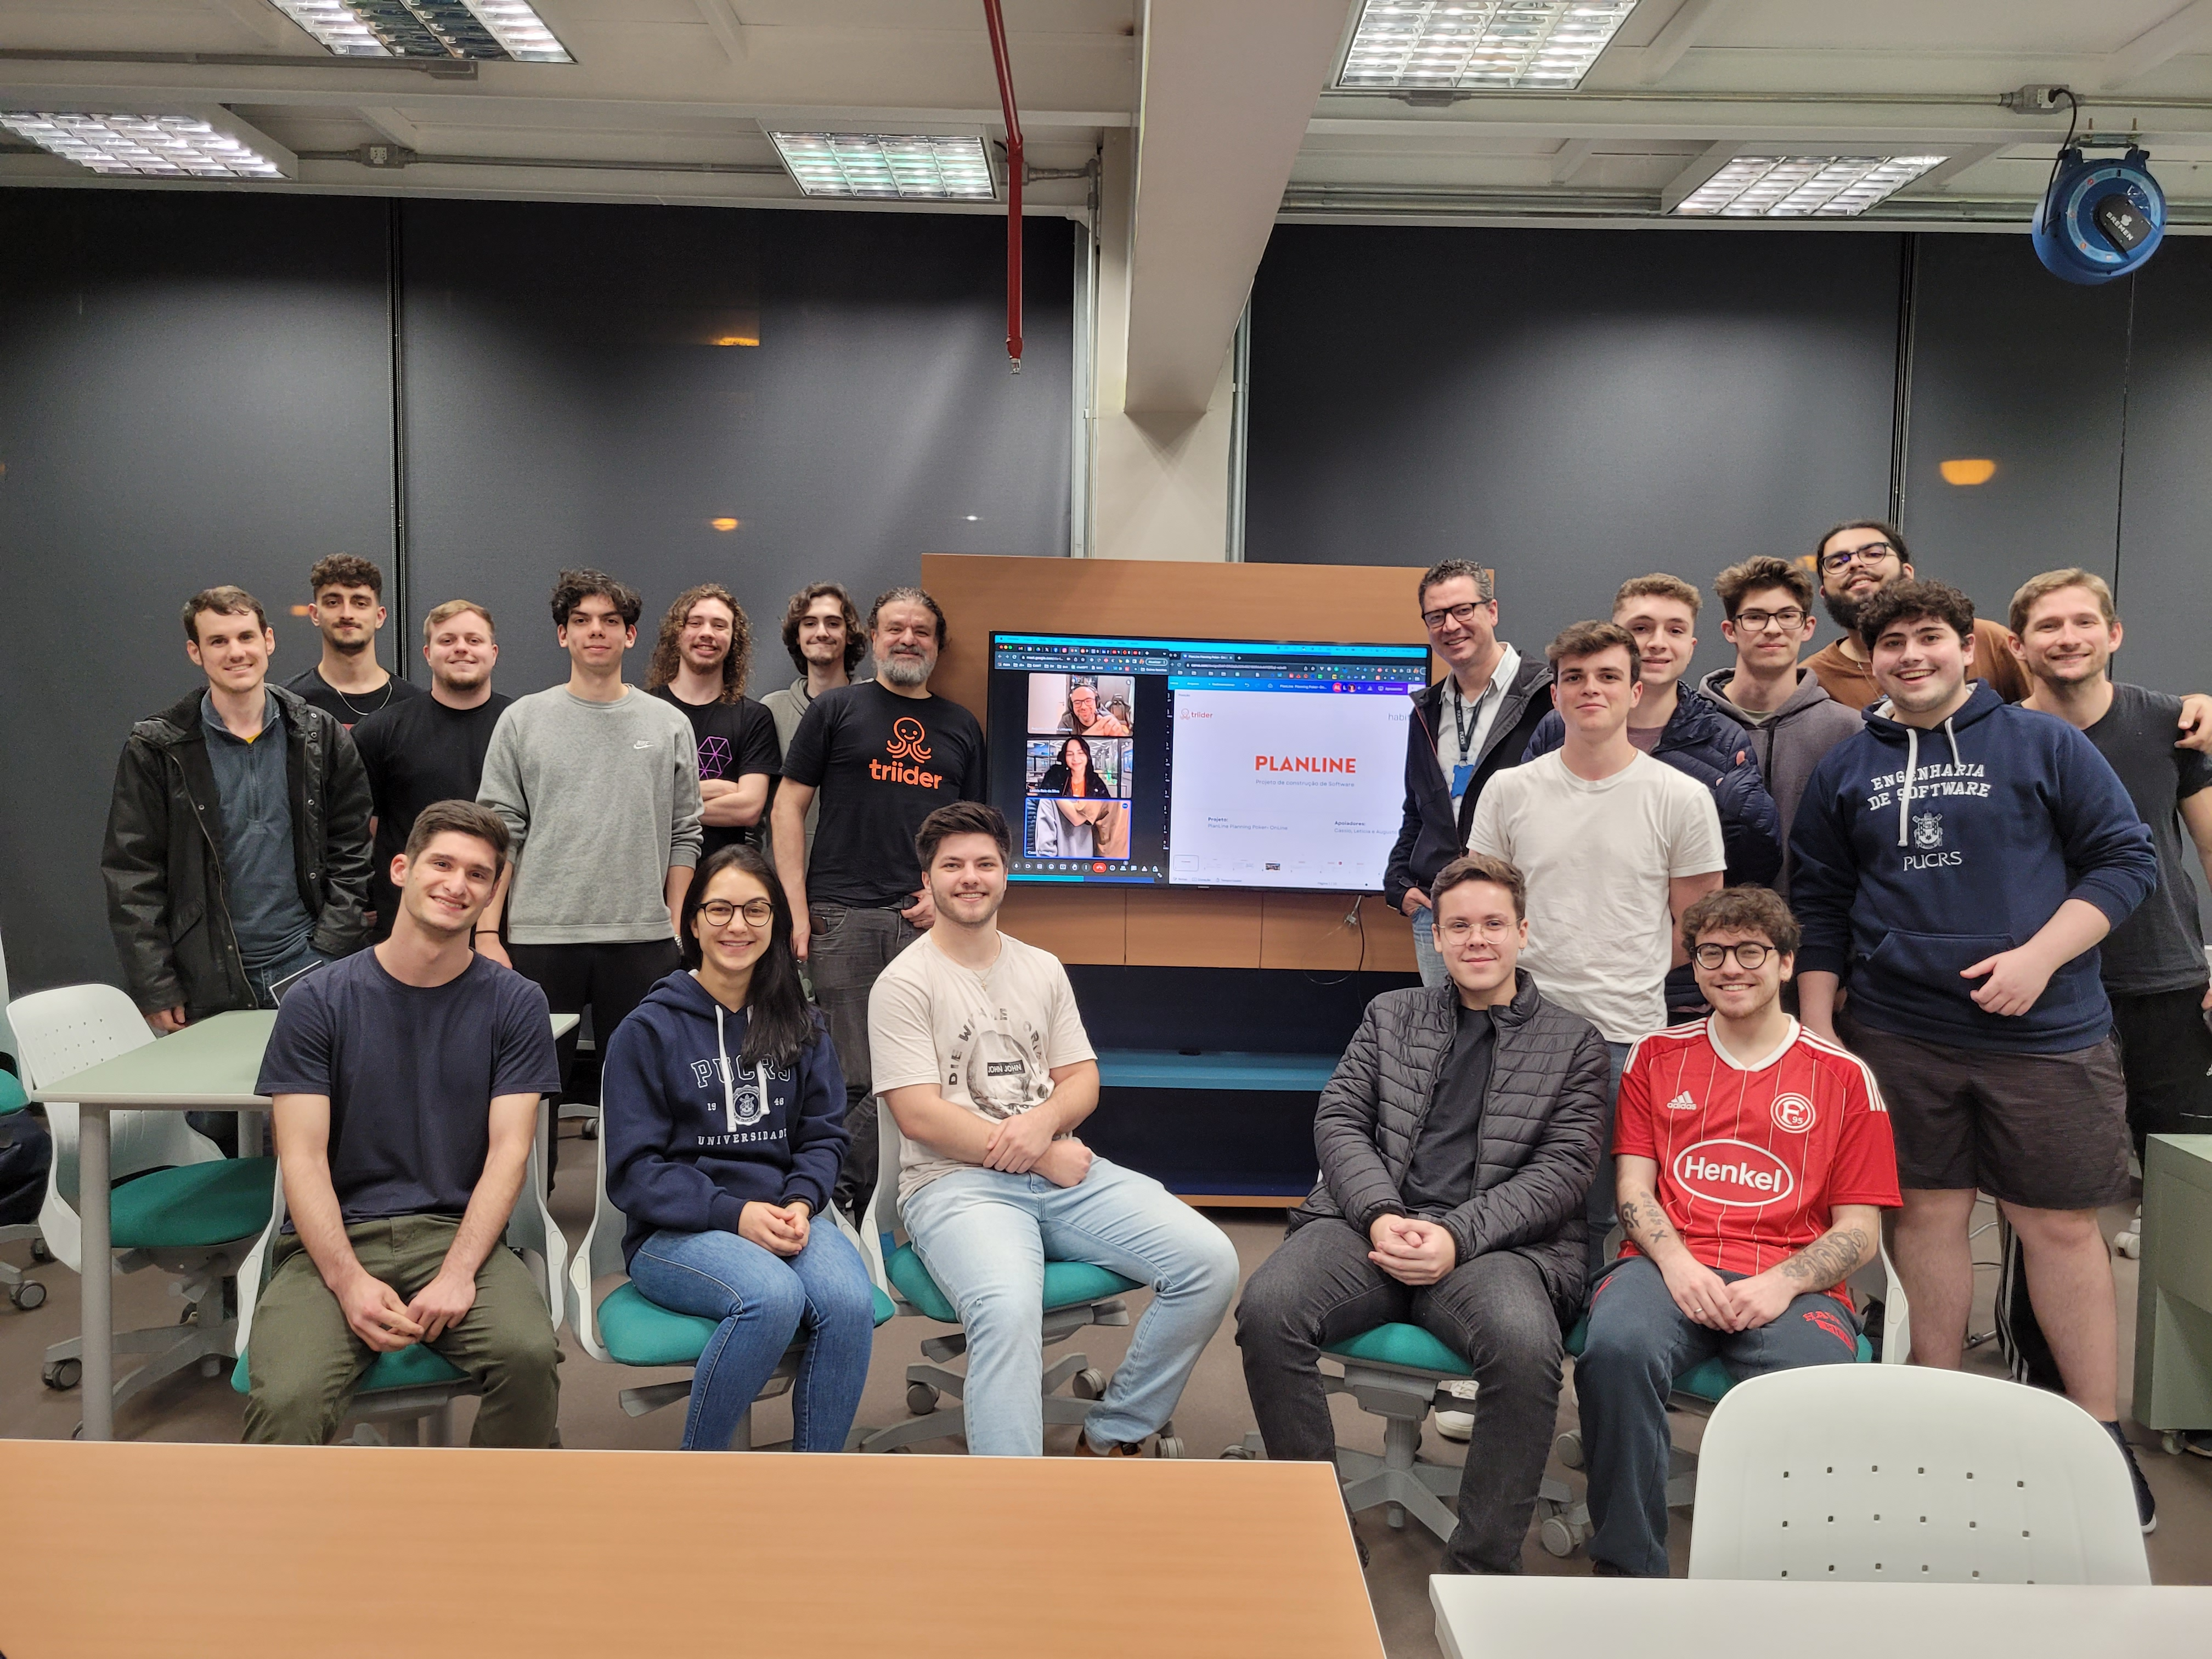
\includegraphics[width=0.9\linewidth,height=0.34\textheight,keepaspectratio]{conteudo/2 - ages I/conteudo/figures/equipe-planline.jpg}
    \legend{Fonte: \href{https://tools.ages.pucrs.br/planline/wiki/-/wikis/home}{wiki do projeto PlanLine}.}
\end{figure}

\section[Desenvolvimento do Projeto]{Desenvolvimento do Projeto}

\subsection{Repositório do Código Fonte do Projeto}

Para organizar o desenvolvimento do Plan Line, a equipe optou por separar o projeto em quatro repositórios principais: Wiki, \textit{backend}, \textit{mobile} e \textit{web}. Essa divisão ajudou a manter o projeto mais encapsulado, facilitando a organização das responsabilidades e a consulta das informações técnicas por frente de desenvolvimento.

{\footnotesize
\begin{itemize}
    \item Wiki: \url{https://tools.ages.pucrs.br/planline/wiki}
    \item \textit{Backend}: \url{https://tools.ages.pucrs.br/planline/backend}
    \item \textit{Mobile}: \url{https://tools.ages.pucrs.br/planline/mobile}
    \item \textit{Web}: \url{https://tools.ages.pucrs.br/planline/web}
\end{itemize}
}

A Wiki foi utilizada como fonte de documentação do projeto, concentrando informações sobre arquitetura, banco de dados, protótipos e decisões técnicas. Os demais repositórios separavam as camadas de implementação da solução, o que contribuiu para uma organização mais clara do trabalho.

\subsection{Banco de Dados Utilizado}

O projeto utilizou Firebase para gerenciamento das sessões e PostgreSQL para armazenamento dos dados gerais da aplicação. Essa composição buscava atender às necessidades específicas do sistema, que envolvia sessões de votação em tempo real e persistência estruturada de informações relacionadas às histórias, usuários e resultados.

As informações sobre o banco de dados foram documentadas na Wiki do projeto:

{\footnotesize
\begin{itemize}
    \item Banco de dados: \url{https://tools.ages.pucrs.br/planline/wiki/-/wikis/banco_dados}
\end{itemize}
}

A Figura~\ref{fig:planline-banco-dados} apresenta a modelagem documentada para o projeto. As relações entre usuários, equipes, histórias, tarefas e votos ajudam a compreender como os dados das estimativas se conectam à organização dos projetos e das \textit{sprints}.

\begin{figure}[!htbp]
    \centering
    \caption{Modelagem do banco de dados do Plan Line}
    \label{fig:planline-banco-dados}
    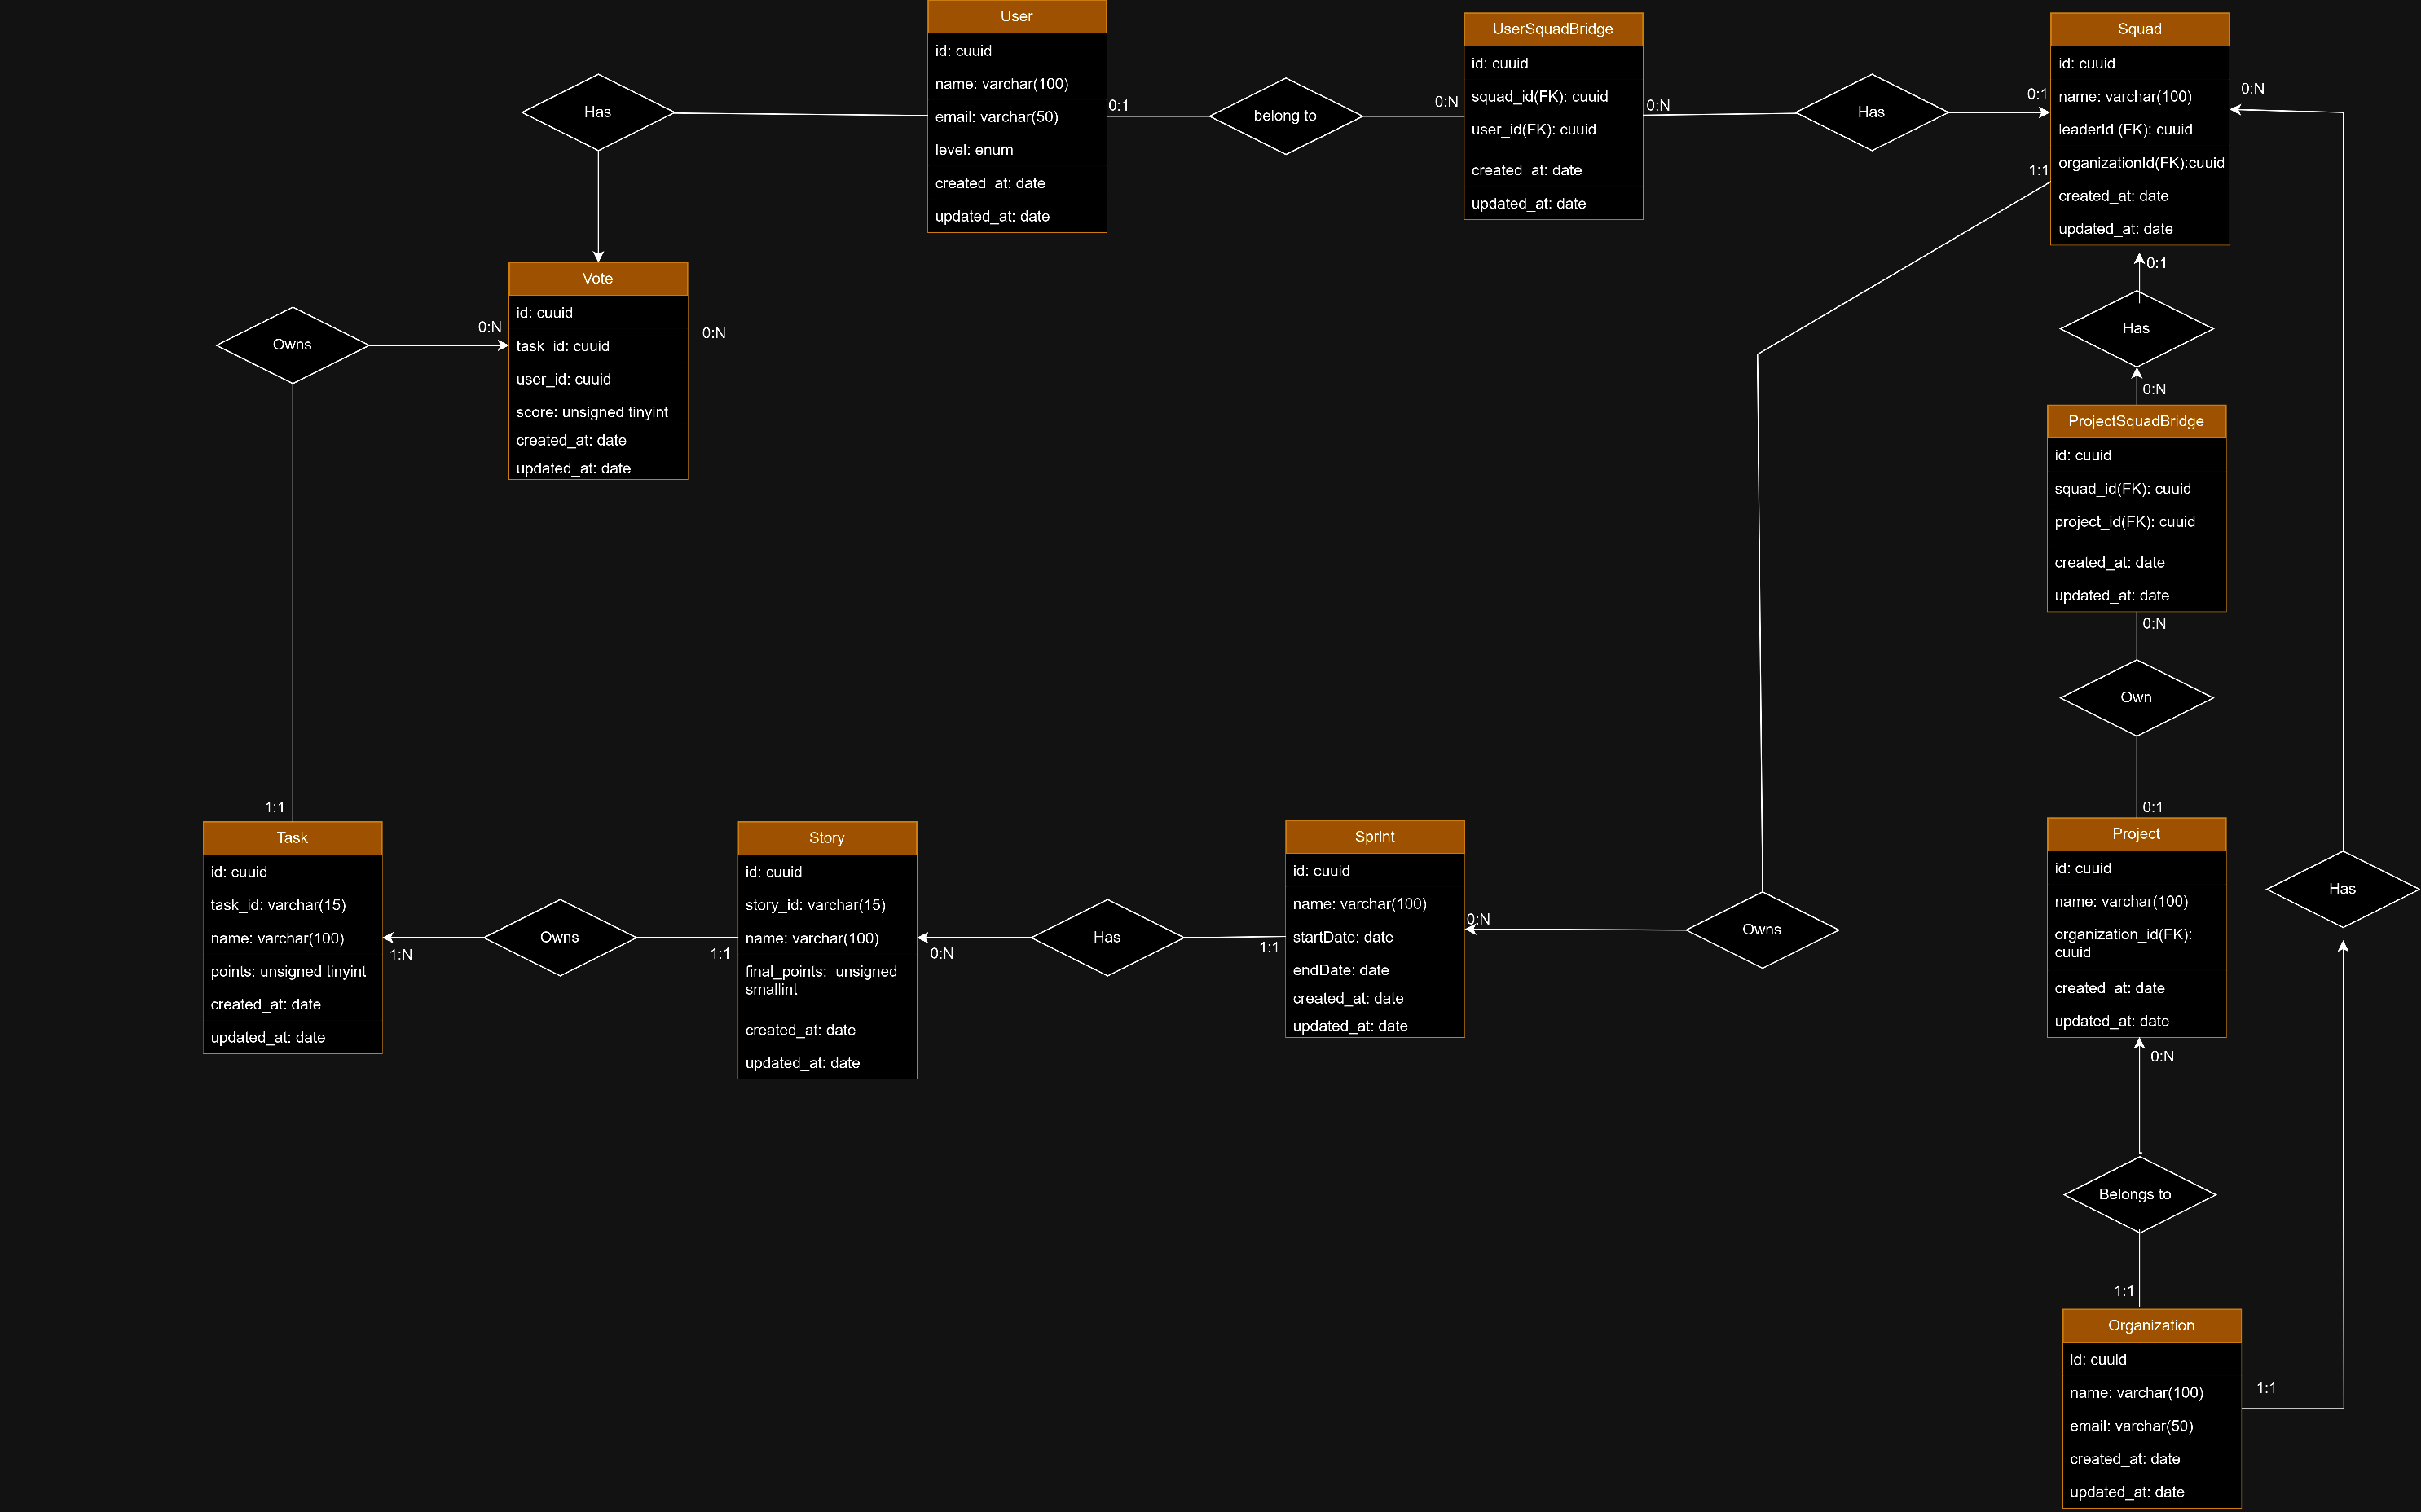
\includegraphics[width=\linewidth,height=0.55\textheight,keepaspectratio]{conteudo/2 - ages I/conteudo/figures/banco-dados-planline.pdf}
    \legend{Fonte: \href{https://tools.ages.pucrs.br/planline/wiki/-/wikis/banco_dados}{wiki do projeto PlanLine}.}
\end{figure}

\subsection{Arquitetura Utilizada}

A arquitetura do Plan Line foi baseada em \textit{Clean Architecture}, separando regras de negócio, infraestrutura e interfaces. Para uma equipe em formação, essa organização ajudou a compreender a divisão de responsabilidades no código.

A arquitetura foi documentada na \href{https://tools.ages.pucrs.br/planline/wiki/-/wikis/arquitetura}{wiki do projeto}.

A Figura~\ref{fig:planline-arquitetura} complementa a descrição da organização do código com a visão de implantação. O diagrama mostra as aplicações \textit{web} e \textit{mobile} e sua comunicação com o \textit{backend} e os serviços de dados utilizados pelo projeto.

\begin{figure}[!htbp]
    \centering
    \caption{Arquitetura de implantação do Plan Line}
    \label{fig:planline-arquitetura}
    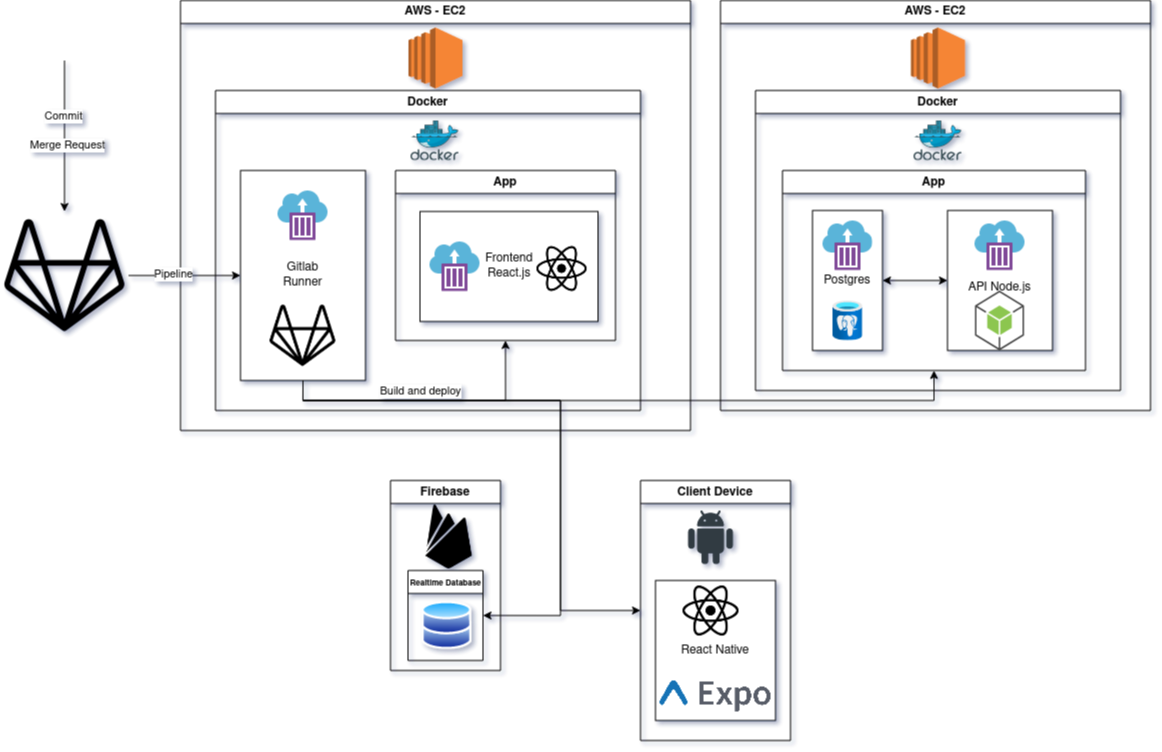
\includegraphics[width=0.95\linewidth,height=0.48\textheight,keepaspectratio]{conteudo/2 - ages I/conteudo/figures/arquitetura-planline.png}
    \legend{Fonte: \href{https://tools.ages.pucrs.br/planline/wiki/-/wikis/arquitetura}{wiki do projeto PlanLine}.}
\end{figure}

\subsection{Protótipos das Telas Desenvolvidas}

Os protótipos das telas foram desenvolvidos no Figma com apoio da \textit{designer} da Triider. Essa etapa foi importante para alinhar expectativas com os \textit{stakeholders} e orientar a implementação das interfaces \textit{web} e \textit{mobile}. Os \textit{mockups} também ajudaram a equipe a compreender melhor os fluxos esperados para criação de sessões, participação nas votações e visualização dos resultados.

{\footnotesize
\begin{itemize}
    \item \textit{Mockups}: \url{https://tools.ages.pucrs.br/planline/wiki/-/wikis/mockups}
\end{itemize}
}

A Figura~\ref{fig:planline-votacao} mostra uma das telas da aplicação \textit{web} demonstrada na wiki. A apresentação das histórias e dos resultados da votação permite visualizar o objetivo central do produto: apoiar a estimativa coletiva de esforço.

\begin{figure}[htbp]
    \centering
    \caption{Tela de votação e resultados do Plan Line}
    \label{fig:planline-votacao}
    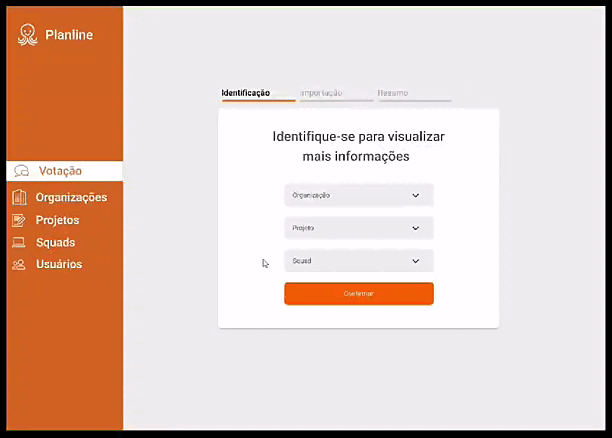
\includegraphics[width=0.9\linewidth,height=0.36\textheight,keepaspectratio]{conteudo/2 - ages I/conteudo/figures/tela-votacao-planline.png}
    \legend{Fonte: primeiro quadro da demonstração web na wiki do Plan Line \cite{planline}.}
\end{figure}

\subsection{Tecnologias Utilizadas}

Na interface \textit{web}, \ac{HTML} estruturou o conteúdo das páginas, \ac{CSS} definiu sua apresentação e JavaScript permitiu implementar interações. TypeScript acrescentou verificação estática de tipos ao desenvolvimento em JavaScript. Essas tecnologias compuseram a base do trabalho com componentes e integração com a aplicação \cite{mdn,typescript}.

React foi utilizado para construir a interface em componentes reutilizáveis, enquanto Tailwind \ac{CSS} apoiou a estilização por meio de classes utilitárias. No \textit{backend}, Node.js permitiu executar JavaScript fora do navegador, e Prisma apoiou o acesso aos dados. A persistência relacional ficou a cargo do PostgreSQL; Firebase foi utilizado na organização das sessões, conforme a documentação do projeto \cite{react,tailwind,node,prisma,postgres,firebase,planline}.

A equipe também trabalhou com importação e exportação de arquivos \texttt{.csv}, criação de \textit{endpoints} e integração entre \textit{frontend} e \textit{backend}. Essas atividades conectavam as tecnologias às necessidades de preparação das sessões, votação e apresentação das estimativas.

No meu caso, o contato com essas tecnologias foi especialmente relevante porque muitas delas estavam além do meu conhecimento inicial. Durante o projeto, precisei estudar os fundamentos de \textit{frontend}, compreender a estrutura de aplicações React, aprender a utilizar Tailwind \ac{CSS} e, posteriormente, iniciar minha aproximação com \textit{backend}, Node.js, Prisma, PostgreSQL e métodos \ac{HTTP}.

\clearpage
\section[Atividades Desempenhadas Pelo Aluno no Projeto]{Atividades Desempenhadas Pelo Aluno no Projeto}

Nesta seção, são descritas as principais atividades realizadas ao longo das \textit{sprints} do projeto Plan Line, considerando tanto as entregas técnicas quanto os aprendizados, dificuldades e reflexões pessoais que surgiram durante o desenvolvimento.

\subsection{Sprint 0 --- 11/08/2023 até 25/08/2023}

O início da \textit{sprint} foi marcado pela apresentação da equipe, o que ajudou a construir uma base de colaboração para o restante do semestre. Em seguida, passamos a discutir as estruturas fundamentais do projeto, incluindo a escolha das tecnologias, a configuração inicial do banco de dados, o levantamento de requisitos e a organização das primeiras histórias de usuário.

Como grande parte das tecnologias escolhidas ainda estava além do meu conhecimento naquele momento, dediquei uma parcela significativa da \textit{sprint} ao estudo. Busquei me familiarizar com \ac{HTML}, \ac{CSS}, JavaScript e os primeiros conceitos de TypeScript. Esse período foi desafiador, pois evidenciou minha inexperiência em desenvolvimento de software, mas também foi muito enriquecedor por me colocar em contato direto com ferramentas utilizadas em um projeto real.

Durante o levantamento de requisitos, a equipe utilizou técnicas como \textit{brainstorming}, \textit{t-shirt sizing} e \textit{planning poker}. Essas práticas ajudaram na pontuação das histórias, na identificação de riscos e na discussão sobre as expectativas dos \textit{stakeholders}. Para mim, foi importante perceber como a definição de requisitos depende não apenas de conhecimento técnico, mas também de comunicação, escuta e capacidade de transformar ideias amplas em tarefas executáveis.

O encerramento da \textit{sprint} incluiu o primeiro encontro com os \textit{stakeholders} Cassio, Letícia e Augusto, representantes da Triider. A reunião foi produtiva, mas também revelou dificuldades de clareza em alguns requisitos, especialmente relacionados à parte web da aplicação. Essa lacuna impactou o andamento inicial do projeto e mostrou a importância de validar entendimento com o cliente desde cedo.

\clearpage
\subsection{Sprint 1 --- 25/08/2023 até 15/09/2023}

Após a retrospectiva da \textit{Sprint} 0, a equipe recebeu autorização para iniciar uma etapa mais voltada ao desenvolvimento. As definições realizadas anteriormente passaram a servir como base para a construção do \textit{software}, e as \textit{sprints} seguintes passaram a exigir maior envolvimento técnico e maior integração entre os membros.

Para esta \textit{sprint}, foram selecionadas duas \textit{user stories} principais, relacionadas à criação de sessões de \textit{Planning Poker} e à possibilidade de participar dessas sessões. Com o uso de tecnologias como Node.js e React, essas tarefas pareciam viáveis, mas ainda exigiam adaptação, especialmente para quem estava começando a desenvolver aplicações \textit{web}.

Inicialmente, minha intenção era contribuir com o \textit{backend} do projeto. No entanto, por causa da minha inexperiência com Node.js, optei por concentrar meus esforços no \textit{frontend}, trabalhando na criação de telas para a parte \textit{web} da aplicação. Fui designado, junto com outros integrantes da \ac{AGES} I, para desenvolver o menu lateral do projeto.

Essa mudança de foco acabou sendo positiva. A tarefa do menu lateral me proporcionou uma oportunidade concreta de aprendizado em React e Tailwind \ac{CSS}. Durante a \textit{sprint}, consegui compreender melhor a organização de componentes, a estilização com classes utilitárias e a importância de manter coerência visual entre as telas. Consegui entregar essa tarefa antes do prazo e, no tempo restante, precisei equilibrar a dedicação à \ac{AGES} com outras disciplinas da faculdade.

O encerramento da \textit{sprint} contou com o segundo encontro com os \textit{stakeholders}, dessa vez sem a presença do Cassio. A reunião foi bastante produtiva e os clientes demonstraram satisfação com as entregas realizadas. Houve pequenas discordâncias relacionadas ao \textit{design}, mas elas foram resolvidas sem grandes impactos no andamento do projeto.

Ao final da \textit{sprint}, celebramos um resultado muito positivo. Além de cumprir as metas estabelecidas, a equipe conseguiu avançar em outras frentes, incluindo telas voltadas para dispositivos móveis. Para mim, essa \textit{sprint} marcou um avanço importante na confiança como desenvolvedor. A experiência com React e Tailwind \ac{CSS} foi desafiadora, mas mostrou que eu era capaz de aprender tecnologias novas e contribuir com uma entrega concreta dentro de um projeto real.

\clearpage
\subsection{Sprint 2 --- 15/09/2023 até 06/10/2023}

Após a retrospectiva da \textit{Sprint} 1, a equipe iniciou uma nova fase buscando aplicar as melhorias identificadas e manter o alinhamento com os objetivos do projeto. A \textit{Sprint} 2 representou uma continuação estratégica do desenvolvimento, mas também trouxe desafios mais intensos, especialmente relacionados ao \textit{backend} e à gestão de tempo.

Nesta \textit{sprint}, foram definidas duas \textit{user stories} principais. A primeira envolvia a visualização de informações da sessão, enquanto a segunda tratava da importação de arquivos \texttt{.csv}. Diferentemente da \textit{sprint} anterior, a ênfase desta etapa recaiu mais sobre o \textit{backend} do que sobre o \textit{frontend}, o que representou um desafio significativo para mim.

Durante a \textit{sprint}, enfrentei dificuldades para contribuir de forma mais consistente. O primeiro motivo foi minha pouca experiência com \textit{backend}, especialmente com Node.js. O segundo foi a sobrecarga de provas e trabalhos no meio do semestre, que tornou mais difícil administrar o tempo dedicado às atividades da \ac{AGES}.

Mesmo com essas limitações, consegui desenvolver uma familiaridade inicial com Node.js, aprendizado que se mostrou importante para as \textit{sprints} seguintes. Minhas contribuições foram mais limitadas do que eu gostaria, mas a \textit{sprint} ainda teve valor formativo por me expor a uma frente técnica diferente e por evidenciar a necessidade de ampliar minha atuação além do \textit{frontend}.

As dificuldades de gestão de tempo não foram exclusivas minhas. A equipe como um todo enfrentou problemas nesse aspecto, o que impactou o projeto. Após o bom desempenho da \textit{Sprint} 1, percebi que houve certo relaxamento coletivo, resultando em contratempos. Embora esses problemas não tenham comprometido de forma definitiva o projeto, funcionaram como um alerta importante sobre a necessidade de disciplina e acompanhamento contínuo.

O encerramento da \textit{sprint} ocorreu na terceira reunião com os \textit{stakeholders}. Apesar das dívidas técnicas existentes, a reunião foi tranquila. Os membros mais experientes conseguiram transmitir confiança aos \textit{stakeholders}, demostrando que a equipe tinha condições de contornar os desafios enfrentados. Também ficou claro que esse período do semestre costuma ser naturalmente mais difícil em projetos \ac{AGES}, devido à concentração de demandas acadêmicas.

\clearpage
\subsection{Sprint 3 --- 06/10/2023 até 27/10/2023}

Após a retrospectiva da \textit{Sprint} 2, a equipe iniciou a nova fase com uma postura mais séria e renovada. Diante dos desafios enfrentados anteriormente, encaramos a \textit{Sprint} 3 como uma oportunidade de corrigir problemas de organização e avançar de forma mais consistente. Além disso, o período mais intenso de provas e trabalhos havia passado, o que permitiu maior dedicação ao projeto.

Para esta \textit{sprint}, optamos por trabalhar em três \textit{user stories}. Além da continuidade da história relacionada à visualização de informações da sessão, foram incluídas tarefas de votação, cadastro e visualização de informações. Embora o \textit{backend} ainda tivesse grande peso, a \textit{sprint} apresentou uma distribuição mais equilibrada entre \textit{frontend} e \textit{backend}, o que facilitou minha participação inicial.

Na primeira metade da \textit{sprint}, concentrei-me no \textit{frontend}. Trabalhei na inserção de componentes em telas de gerenciamento e na criação de uma tabela genérica para essas telas. Apesar de já possuir maior familiaridade com React e Tailwind \ac{CSS}, comecei a perceber que não estava totalmente satisfeito atuando apenas nessa frente. Essa percepção me levou a sair da zona de conforto e buscar envolvimento com \textit{backend}.

Na parte final da \textit{sprint}, assumi uma tarefa relacionada à criação de \textit{endpoints} para operações de \ac{CRUD}. Com o apoio de colegas mais experientes da \ac{AGES} II, tive contato com conceitos importantes de desenvolvimento \textit{backend} para aplicações web, como métodos \ac{HTTP}, Prisma, PostgreSQL e Node.js. Até o final da \textit{sprint}, consegui avançar de forma mais independente na conclusão dessa tarefa, consolidando um aprendizado técnico importante.

A equipe trabalhou intensamente durante essa \textit{sprint}. Mesmo sem concluir integralmente todas as \textit{user stories}, as pendências restantes estavam relacionadas a detalhes menores. Ainda assim, voltamos a cometer problemas de gestão de tempo, deixando tarefas importantes, como o \ac{CRUD}, para muito próximo do prazo final. Conseguimos contornar a situação pela dedicação da equipe, mas ficou evidente que esforço de última hora não deveria ser tratado como solução recorrente.

Na quarta reunião com os \textit{stakeholders}, apresentamos as entregas e as pendências, atendendo às expectativas dos clientes e aumentando nossa confiança para a etapa final.

\clearpage
\subsection{Sprint 4 --- 27/10/2023 até 17/11/2023}

Após a retrospectiva da \textit{Sprint} 3, iniciamos a quinta e última \textit{sprint} do projeto. O progresso alcançado anteriormente aumentou a motivação da equipe e criou uma expectativa positiva para a entrega final, inclusive com o desejo de disputar o prêmio de melhor projeto.

Nesta \textit{sprint}, além de tratar pequenas dívidas técnicas acumuladas nas etapas anteriores, incorporamos a última \textit{user story} solicitada pelos \textit{stakeholders}. Essa demanda envolvia a implementação da exportação de dados em formato \texttt{.csv}, contendo as informações processadas pela aplicação. A \textit{sprint} teve foco predominante em \textit{backend} e correção de bugs, buscando garantir estabilidade e funcionamento completo antes da entrega.

Durante essa etapa, minha atuação foi mais voltada a suporte do que ao desenvolvimento direto de novas funcionalidades. Contribuí em alguns ajustes de \textit{frontend}, especialmente relacionados à definição final do \textit{design}, mas minha principal responsabilidade foi auxiliar colegas da \ac{AGES} I na configuração do ambiente de trabalho e do banco de dados. Dediquei tempo a orientar outros membros para que pudessem trabalhar com mais autonomia e eficiência.

No encerramento da \textit{sprint}, acompanhei colegas mais experientes lidando com questões relacionadas ao Firebase, o que me proporcionou uma base inicial para explorar tecnologias semelhantes no futuro. Mesmo sem assumir grandes tarefas novas de implementação, considero que essa atuação de apoio foi importante para a equipe e para meu desenvolvimento, pois reforçou a importância de compartilhar conhecimento e ajudar a destravar o trabalho coletivo.

De modo geral, esta \textit{sprint} foi mais leve do que as anteriores. Isso ocorreu principalmente porque o projeto já estava bem encaminhado, reduzindo a pressão por entregas de última hora. Além disso, o final do semestre e a proximidade das férias contribuíram para um clima mais tranquilo dentro da equipe.

O projeto foi encerrado em 17/11/2023, durante a quinta e última reunião com os \textit{stakeholders}. A reunião foi positiva, e o projeto foi aceito por completo. No entanto, houve uma situação inesperada: fomos informados de que Cassio e Letícia, dois dos \textit{stakeholders} com quem havíamos trabalhado, haviam sido desligados da Triider. Ainda assim, ambos participaram da reunião, demostrando respeito e apreço pelo trabalho desenvolvido pela equipe.

A \textit{Sprint} 4 encerrou o projeto de forma positiva, embora com essa reviravolta inesperada. A equipe pôde concluir a entrega com mais tranquilidade, apoiada pelo avanço substancial das \textit{sprints} anteriores. Para mim, essa fase reforçou que contribuir para um projeto não significa apenas implementar funcionalidades, mas também apoiar colegas, compartilhar conhecimento e colaborar para que o produto chegue ao fim com qualidade.


\section{Conclusão}

O Plan Line foi meu primeiro contato com o desenvolvimento de um projeto real. Cheguei à AGES I sem domínio das tecnologias utilizadas e precisei estudar enquanto aprendia a contribuir em equipe. Essa experiência me ajudou a compreender tanto a implementação quanto as responsabilidades envolvidas em uma entrega para clientes.

No início, dediquei tempo aos fundamentos de HTML, CSS, JavaScript e TypeScript. O trabalho no menu lateral, com React e Tailwind CSS, trouxe mais confiança para construir uma interface e concluir uma tarefa dentro do prazo. Posteriormente, o contato com endpoints, métodos HTTP, Prisma e PostgreSQL permitiu experimentar o backend e descobrir uma afinidade que influenciou minhas escolhas nos projetos seguintes.

Minha principal autocrítica foi a organização do tempo. Na Sprint 2, contribuí menos do que gostaria por dificuldades técnicas e pela sobrecarga acadêmica. Reconheço que poderia ter buscado orientação e comunicado os obstáculos mais cedo. A equipe também deixou tarefas importantes para perto dos prazos, o que reduziu o tempo de revisão e exigiu esforço adicional nas entregas.

Como aprendizado de colaboração, destaco o apoio recebido dos colegas mais experientes e a oportunidade de, na última sprint, ajudar outros integrantes na configuração do ambiente e do banco. Acompanhar essas dificuldades mostrou que compartilhar conhecimento e esclarecer dúvidas também eram formas de contribuir. As reuniões com os stakeholders ajudaram a perceber a importância de ouvir e ajustar o produto às expectativas dos clientes.

As atividades aproximaram a prática dos conteúdos de programação, banco de dados, requisitos e métodos ágeis. A base teórica começou a fazer sentido em situações concretas, como compreender o fluxo de uma requisição, organizar uma tarefa ou discutir uma funcionalidade. Essa relação entre disciplinas e projeto foi um dos principais resultados formativos da experiência.

O Plan Line teve o valor particular de iniciar minha vivência profissional e revelar meu interesse pelo backend. Na comparação entre as quatro AGES, considero o ReadRace a melhor experiência para mim, principalmente pelas oportunidades de gestão e evolução pessoal na AGES IV. O aprendizado inicial do Plan Line foi uma base importante para chegar a essa etapa com mais segurança.


  \chapter[AGES II --- Certificações por meio de Blockchain]{AGES II --- Certificações por meio de Blockchain}



\section[Introdução]{Introdução}

No primeiro semestre de 2024, cursei a AGES II no projeto de certificações por meio de Blockchain, sob a orientação do professor Azriel Majdenbaum. O projeto se destacou por sua abordagem diferenciada e pelo desejo que eu tinha de aprofundar meu conhecimento nessa tecnologia. Por isso, decidi que seria minha primeira opção. Ao contrário da AGES anterior, eu ficaria responsável pela criação do banco de dados da aplicação, o que representava um novo desafio para mim.

O conceito central do projeto consistiu na criação de uma blockchain dedicada ao armazenamento de certificações e diplomas emitidos por instituições de ensino. Essa blockchain permitiria que outras entidades, como empresas, pudessem verificar a autenticidade desses documentos de forma segura e confiável. A inspiração para essa ideia surgiu do stakeholder Edimar Luís de Moraes, representante do Instituto de Pesquisas Eldorado, que nos explicou durante a nossa primeira reunião com ele as especificações do projeto.

A primeira reunião da nossa equipe aconteceu no primeiro dia de AGES e foi muito importante pois foi nela que pudemos nos conhecer de uma forma geral, nossas formações e interesses. Além da apresentação começamos a nos preparar para a primeira reunião com o stakeholder o qual formalizariamos os requisitos do projeto.

Depois de uma semana de preparação intensiva, tivemos nossa primeira reunião com o stakeholder. Foi uma sessão longa e produtiva, na qual discutimos e esclarecemos o escopo do projeto. Diferentemente do meu projeto anterior, no qual os requisitos já estavam bem definidos, desta vez houve uma colaboração mais estreita entre o time e o stakeholder na modelagem do projeto. A troca de ideias foi bastante enriquecedora e contribuiu significativamente para um entendimento mais profundo das necessidades e objetivos do projeto. Com o término desta reunião, passavamos assim para a sprint 0.

A equipe responsável pelo projeto é apresentada na Figura~\ref{fig:blockchain-equipe}. A convivência entre alunos de diferentes níveis da AGES permitiu dividir responsabilidades de desenvolvimento, modelagem, arquitetura e gestão.

\begin{figure}[H]
    \centering
    \caption{Equipe do projeto Certificação por meio de Blockchain}
    \label{fig:blockchain-equipe}
    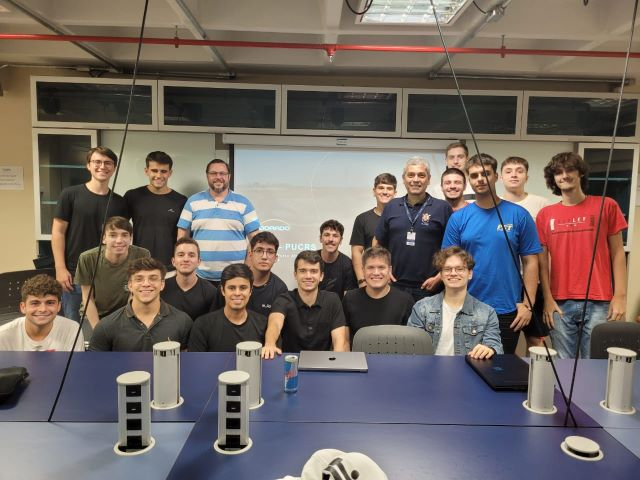
\includegraphics[width=0.8\textwidth]{A.jpg}
    \legend{Fonte: \href{https://tools.ages.pucrs.br/certifica-o-por-meio-de-blockchain/blockchain-wiki/-/wikis/home}{wiki do projeto Certificação por meio de Blockchain}.}
\end{figure}


\section[Desenvolvimento do Projeto]{Desenvolvimento do Projeto}

\subsection{Repositório do Código Fonte do Projeto}
  https://tools.ages.pucrs.br/certifica-o-por-meio-de-blockchain/blockchain-wiki

  https://tools.ages.pucrs.br/certifica-o-por-meio-de-blockchain/blockchain-api

  https://tools.ages.pucrs.br/certifica-o-por-meio-de-blockchain/blockchain-ui

  https://tools.ages.pucrs.br/certifica-o-por-meio-de-blockchain/ethereum-contract

  https://tools.ages.pucrs.br/certifica-o-por-meio-de-blockchain/ethereum-bridge

  Nosso projeto foi dividido em cinco repositórios diferentes. O primeiro e padrão da Wiki, o segundo do backend, o terceiro ao frontend , o quarto a API do contrato da nossa aplicação na etherium e por ultimo a "ponte" que liga a blockchain a nossa aplicação backend.

\subsection{Banco de Dados Utilizado}
 \href{https://tools.ages.pucrs.br/certifica-o-por-meio-de-blockchain/blockchain-wiki/-/wikis/Banco-de-Dados}{Documentação do banco de dados na wiki do projeto.}

 Para a nossa aplicação usamos o banco de dados relacional Postgrees. Para ele criamos quatro entidades, Certificado, Empresa, Usuário e Permissão. Além dos relcionamentos básicos de conexão entre as entidades criamos um levando em consideração a geração de logs. Além do Postgrees usamos o firebase para a autenticação de usuários.
\sloppy
O modelo lógico apresentado na Figura~\ref{fig:blockchain-banco-dados} detalha a organização das tabelas e de seus relacionamentos. Esse artefato complementa o relato sobre a modelagem realizada com meu colega e ajuda a explicar a associação entre empresas, usuários, permissões e certificados.

\begin{figure}[H]
    \centering
    \caption{Modelo lógico do banco de dados do projeto Certificação por meio de Blockchain}
    \label{fig:blockchain-banco-dados}
    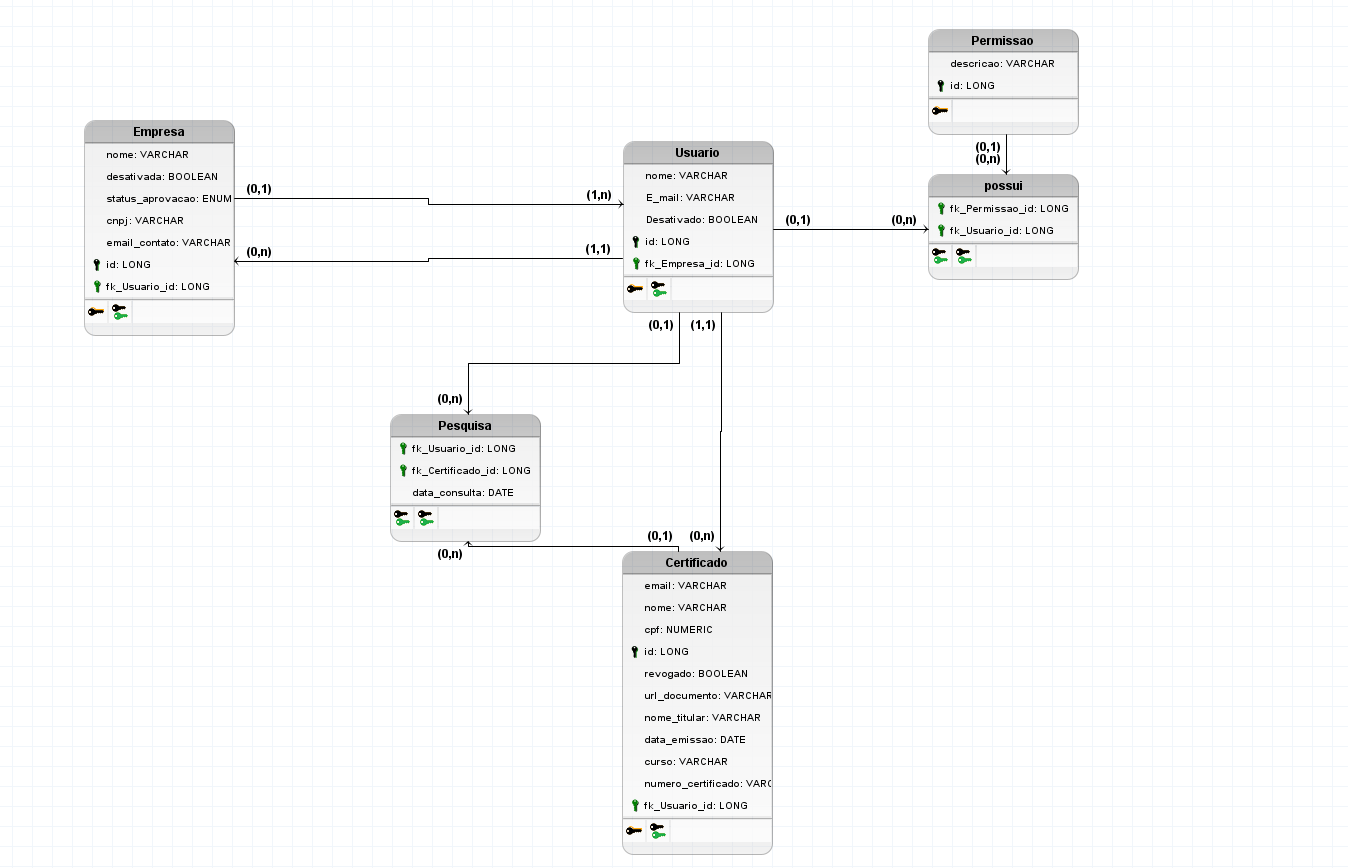
\includegraphics[width=\linewidth,height=0.53\textheight,keepaspectratio]{conteudo/3 - ages II/conteudo/figures/banco-dados-blockchain.png}
    \legend{Fonte: \href{https://tools.ages.pucrs.br/certifica-o-por-meio-de-blockchain/blockchain-wiki/-/wikis/Banco-de-Dados}{wiki do projeto Certificação por meio de Blockchain}.}
\end{figure}

\subsection{Arquitetura Utilizada}
 https://tools.ages.pucrs.br/certifica-o-por-meio-de-blockchain/blockchain-wiki/-/wikis/arquitetura

 https://tools.ages.pucrs.br/certifica-o-por-meio-de-blockchain/blockchain-wiki/-/wikis/infraestrutura

 Para nossa arquitetura, organizamos o sistema em três camadas distintas: o backend, o frontend e a blockchain. A interação entre o frontend e a blockchain ocorria exclusivamente através do backend. Isso significa que todas as requisições e operações realizadas pelo frontend relacionadas à blockchain passavam primeiro pelo backend, que atuava como intermediário. Essa abordagem permitiu maior controle, segurança e facilita a integração entre as diferentes partes do sistema, garantindo que as operações na blockchain sejam realizadas de maneira eficiente e segura, sem expor diretamente o frontend à complexidade da infraestrutura blockchain.

A Figura~\ref{fig:blockchain-arquitetura} apresenta os componentes da solução, identificada como AuthLink na documentação. A separação entre interface, API, banco de dados e blockchain evidencia o papel do backend na intermediação das operações solicitadas pelos usuários.

\begin{figure}[H]
    \centering
    \caption{Diagrama de componentes do AuthLink}
    \label{fig:blockchain-arquitetura}
    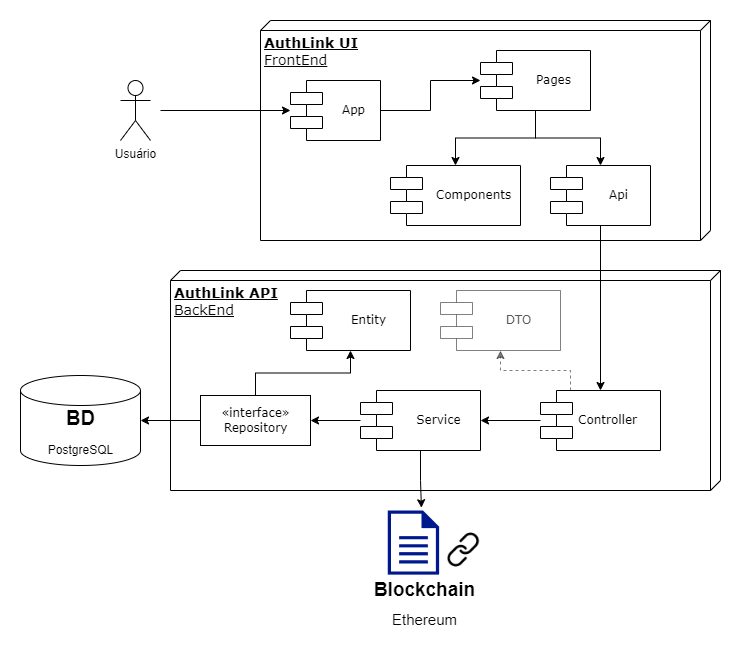
\includegraphics[width=0.85\linewidth,height=0.49\textheight,keepaspectratio]{conteudo/3 - ages II/conteudo/figures/arquitetura-blockchain.png}
    \legend{Fonte: \href{https://tools.ages.pucrs.br/certifica-o-por-meio-de-blockchain/blockchain-wiki/-/wikis/arquitetura}{wiki do projeto Certificação por meio de Blockchain}.}
\end{figure}

\subsection{Protótipos das Telas Desenvolvidas}
\sloppy
  https://tools.ages.pucrs.br/certifica-o-por-meio-de-blockchain/blockchain-wiki/-/wikis/design/mockups

  Para a criação de mockups, usamos o figma. Mais detalhes sobre os mockups, utilize o link acima.

\subsection{Tecnologias Utilizadas}
  https://tools.ages.pucrs.br/certifica-o-por-meio-de-blockchain/blockchain-wiki/-/wikis/arquitetura
  
  Para o frontend usamos TypeScript e  o framework React. Para o backend usamos o Java 21 em conjunto com o  framework SpringBoot. Para a blockchain, além de usarmos a Etherium, usamos sua linguagem Solidity para a criação de contratos.

\clearpage
\section[Atividades Desempenhadas Pelo Aluno no Projeto]{Atividades Desempenhadas Pelo Aluno no Projeto}

\subsection{Sprint 0}

A \textit{Sprint} 0 ocorreu aproximadamente entre 8 e 22 de março de 2024. O encerramento em 22 de março consta no relatório da etapa; o início foi situado cerca de duas semanas antes, como referência aproximada. O planejamento previa as especificações iniciais do projeto, incluindo protótipos, tecnologias e fluxo geral da aplicação. Essas atividades foram concluídas, enquanto a implementação das histórias de usuário e a continuidade da modelagem do banco ficaram para a etapa seguinte.

Nas reuniões, discutimos tecnologias, banco de dados e requisitos. Foi um período de estudo e preparação para compreender as partes do produto antes de distribuir as tarefas.

A experiência da \ac{AGES} anterior me ajudou a estudar as tecnologias com mais segurança. A principal novidade era a \textit{blockchain}: procurei entender seu funcionamento, suas possibilidades e limitações e a forma como seria integrada à aplicação. Também estudei os fundamentos de Spring Boot para me familiarizar com o \textit{backend} que utilizaríamos. Esses estudos me permitiram acompanhar melhor as discussões técnicas, ainda que eu precisasse aprofundar o conhecimento durante a implementação.

Minha contribuição se concentrou na modelagem conceitual do banco. Não participei dos protótipos, pois ainda tinha pouca familiaridade com essa atividade. Como as histórias de usuário estavam em definição, o avanço da modelagem dependia do esclarecimento das regras. Entendi que organizar o banco exigia compreender as necessidades da aplicação.

Na segunda reunião com Edimar, apresentamos os protótipos e as histórias de usuário elaboradas pela equipe. O encontro foi mais curto que o anterior, e o \textit{stakeholder} demonstrou satisfação com o progresso, sem solicitar alterações naquele momento. Os colegas da \ac{AGES} IV selecionaram cinco das 12 histórias para a próxima \textit{sprint}, definindo um recorte de implementação mais exigente para o time.

Dois dos quatro integrantes da \ac{AGES} II saíram do projeto nessa etapa. A modelagem ficou sob minha responsabilidade e a de outro colega. Foi necessário reorganizar o trabalho e me adaptar à nova composição do grupo, assumindo mais responsabilidade técnica.

\clearpage
\subsection{Sprint 1}

Após a retrospectiva da \textit{Sprint} 0, a equipe iniciou o desenvolvimento dividida em três subgrupos: \textit{frontend}, \textit{backend} e \textit{blockchain}. Fiquei no \textit{backend}, a área que mais me interessava. Meu objetivo nessa \ac{AGES} era compreender melhor o funcionamento de uma aplicação dessa camada e ampliar a experiência iniciada no projeto anterior.

Continuei a modelagem do banco com meu colega, revisando versões conforme as histórias de usuário mudavam. Definimos quatro entidades principais: Empresa, Usuário, Certificado e Permissão. Discutimos a representação dos usuários e mantivemos a tabela de permissões para facilitar as consultas. Iniciamos também o modelo lógico, que ficou pendente para a próxima \textit{sprint}.

Além da modelagem, implementei uma operação com o método \ac{HTTP} PATCH para rejeitar o cadastro de empresas. Conheci melhor o fluxo das requisições e o uso de Lombok e \ac{JPA}, relacionando objetos de transferência de dados, controladores, serviços e persistência.

Na segunda tarefa, trabalhei com um colega na criação de funcionários de uma empresa por meio do método \texttt{POST}. Durante a implementação, revisamos a modelagem para utilizar uma única entidade de usuários. Ao contrário da tarefa anterior, foi necessário construir mais estruturas desde o início, o que tornou a depuração mais trabalhosa. Utilizei o Postman para verificar as requisições, investigar os problemas e conferir as respostas da \ac{API}. Com esse processo, conseguimos concluir a tarefa antes do congelamento do código.

A \textit{sprint} terminou com a terceira reunião com o \textit{stakeholder}. Apresentamos a evolução do produto e cerca de quatro quintos das tarefas planejadas. Edimar demonstrou satisfação com o progresso, embora tenha manifestado preocupação com o uso de uma \textit{blockchain} pública. A equipe discutiu a abordagem de segurança proposta, e a demonstração foi aprovada. Esse retorno não significava que todos os riscos estivessem resolvidos, mas permitiu alinhar as dúvidas e dar continuidade ao projeto.

A experiência anterior me ajudou a compreender métodos \ac{HTTP} e buscar apoio. Nesta etapa, aprofundei o estudo de Spring Boot e de sua relação com o banco. Minha dificuldade foi combinar requisitos em definição com conhecimento técnico em formação. Aprendi que esclarecer regras e revisar a modelagem são partes da implementação.

\clearpage
\subsection{Sprint 2}

Após a retrospectiva da \textit{Sprint} 1, a equipe estava entusiasmada com o progresso do projeto. A etapa seguinte reunia funcionalidades centrais de certificação, por isso planejamos os próximos passos com atenção às dependências entre \textit{backend}, \textit{frontend} e \textit{blockchain}. Também foi positivo perceber o envolvimento dos colegas, muitos deles em sua primeira participação na \ac{AGES}.

O planejamento incluía operações de cadastro de certificados, que dependiam da integração com a \textit{blockchain}. O subgrupo responsável por essa frente havia decidido trabalhar com uma \textit{sidechain} do Ethereum. Os contratos seriam escritos em Solidity, e a camada de integração intermediaria as operações necessárias. A escolha e a implementação dessa parte ficaram sob responsabilidade daquele subgrupo.

No \textit{backend}, nosso trabalho envolvia conectar os fluxos da interface às operações de certificação, com \textit{endpoints} de registro, consulta e validação e os mecanismos de autenticação e autorização. Também precisaríamos implementar a estrutura do banco de dados cuja modelagem eu e meu colega de \ac{AGES} II estávamos concluindo. A relação entre essas frentes exigia alinhar as regras e as informações necessárias a cada operação.

No início da \textit{sprint}, concluímos a modelagem e começamos a implementar os atributos e relacionamentos no \textit{backend}. Entretanto, as enchentes no Rio Grande do Sul interromperam o andamento do projeto. Ficamos duas semanas sem aulas e pausamos as atividades para lidar com os efeitos da situação, que atingiram a equipe de formas diferentes.

Quando as aulas retornaram de forma remota, percebi desânimo na primeira reunião. Embora eu não tenha sofrido danos materiais, a situação me afetou psicologicamente e coincidiu com uma piora no meu quadro de doença autoimune. Não consegui manter a participação que havia planejado e fiquei sem contribuir até o encerramento da \textit{sprint}. Essa interrupção foi frustrante, pois eu estava envolvido com o projeto e encontrava dificuldade para recuperar o ritmo.

Apesar das limitações, os colegas conseguiram avançar em diversas tarefas. Reconheço o comprometimento da equipe em buscar a melhor entrega possível nas condições daquele momento. O resultado não repetiu o ritmo da \textit{sprint} anterior, mas a adaptação do planejamento permitiu dar continuidade ao trabalho.

Encerramos a etapa em 24 de maio de 2024, em uma videochamada com Edimar. Ainda havia pendências no \textit{backend}, na configuração da \ac{AWS} e na integração com a \textit{blockchain}. O \textit{stakeholder} compreendeu as dificuldades enfrentadas pela equipe e demonstrou satisfação com o progresso apresentado. Esse retorno ajudou a recuperar o ânimo para as próximas etapas.

Minha principal aprendizagem foi reconhecer a necessidade de ajustar os compromissos às condições reais de participação. A \textit{sprint} teve menos entregas do que esperávamos, mas evidenciou a importância do apoio entre os colegas e da comunicação sobre limitações e impedimentos. Pessoalmente, precisei lidar com uma redução de participação que não correspondia à minha disposição inicial. Essa experiência ampliou minha compreensão sobre adaptação e trabalho em equipe diante de situações que não poderiam ser resolvidas apenas com mais esforço técnico.

\clearpage
\subsection{Sprint 3}

Após a reunião com o \textit{stakeholder}, iniciamos os preparativos para a \textit{Sprint} 3. O planejamento incluía consultas, validações e emissão de certificados, além das pendências da etapa anterior. Essas funcionalidades exigiam trabalho no \textit{backend} e no \textit{frontend}, enquanto a integração com a \textit{blockchain} ainda precisava de ajustes.

Como eu havia percebido dificuldades com Spring Boot na primeira \textit{sprint}, dediquei a primeira semana ao estudo do \textit{framework}. Retomei conceitos de organização da aplicação e de processamento das requisições para me preparar para as tarefas. Esse período foi importante para compreender melhor o código existente e buscar soluções com mais autonomia, sem deixar de pedir apoio quando necessário.

Minha primeira tarefa foi implementar a listagem dos certificados de uma empresa. Ela reuniu aspectos que eu ainda não havia trabalhado em conjunto, como paginação, cabeçalhos das requisições e autenticação. Pedi orientação aos colegas de \ac{AGES} IV, que me ajudaram a entender esses pontos. Em seguida, configurei os \textit{endpoints}, as requisições paginadas e os cabeçalhos necessários, além do acesso ao banco de dados. O trabalho e os testes permitiram aplicar o que eu havia estudado no início da \textit{sprint}.

A segunda tarefa foi implementar a exclusão lógica de funcionários. Em vez de remover o usuário do banco, a operação alteraria um atributo para indicar se sua conta estava ativa. Essa escolha preservava os certificados associados ao funcionário e evitava os efeitos que a remoção do registro poderia causar nos relacionamentos. Trabalhei no \textit{endpoint}, na autenticação, na lógica do serviço e na atualização do estado do usuário no banco. A experiência da tarefa anterior e a orientação recebida ajudaram a conduzir essa implementação com mais segurança.

Também enfrentei conflitos nas alterações que enviei para integração. Não consegui resolvê-los sozinho, e precisei do apoio de colegas mais experientes para concluir a integração. Foi um período frustrante, pois as funcionalidades já haviam exigido estudo e implementação, mas ainda dependiam dessa etapa para entrar no projeto. A situação reforçou que desenvolver uma tarefa inclui cuidar de sua integração com o trabalho da equipe.

A \textit{sprint} terminou com a penúltima reunião com Edimar. As aulas presenciais já haviam retornado, mas ele não pôde comparecer pessoalmente. A equipe apresentou praticamente todas as entregas previstas, com exceção da implantação na \ac{AWS}, que continuou pendente. Essa frente estava concentrada nos integrantes da \ac{AGES} III, que também acumulavam outras demandas. O \textit{stakeholder} demonstrou satisfação com o progresso apresentado.

Na retrospectiva, discutimos a demora das revisões de código, especialmente no \textit{backend}. Minhas solicitações de integração haviam ficado pendentes por um período prolongado, o que contribuiu para a dificuldade que enfrentei. A equipe reconheceu o problema e combinou dar mais atenção às revisões na última \textit{sprint}. Esse alinhamento mostrou a importância de reservar tempo para acompanhar as alterações dos colegas, além de concluir as próprias tarefas.

Para mim, foi uma etapa de consolidação técnica. Aprofundei o contato com Spring Boot, paginação, autenticação e exclusão lógica, mas também aprendi sobre os limites da minha autonomia e sobre a importância de buscar orientação. O apoio recebido foi decisivo para resolver os conflitos e concluir as entregas. A experiência reforçou a necessidade de combinar estudo individual, comunicação e revisão contínua durante o desenvolvimento.

\clearpage
\subsection{Sprint 4}

A \textit{Sprint} 4 foi encerrada em 5 de julho de 2024. O escopo incluía a resolução de débitos técnicos, a geração de \textit{logs} e o cadastramento de certificados em lotes. A equipe concluiu as atividades previstas, tendo como uma das dificuldades a paralelização das operações de cadastro.

Minha atuação se concentrou nos débitos técnicos das etapas anteriores, enquanto outros colegas do \textit{backend} assumiram as funcionalidades principais. Escolhi trabalhar nas operações de cadastro e remoção de certificados, que aguardavam a conclusão do processamento na \textit{blockchain} antes de prosseguir. Durante o desenvolvimento, eu estimava esse tempo em cerca de 15 segundos por operação; trata-se de uma percepção daquele contexto, sem medição formal. A espera prejudicava a resposta da aplicação e motivou a revisão desse fluxo.

Comecei a reestruturar o código para permitir o processamento assíncrono. O objetivo era executar as operações em segundo plano, mantendo a aplicação disponível para atender outras requisições. Esse trabalho exigiu considerar a diferença entre receber uma solicitação e concluir uma operação na \textit{blockchain}, pois as duas etapas deixariam de ocorrer no mesmo fluxo sequencial.

Utilizei os recursos do Spring Boot para publicação e tratamento de eventos e adaptei o controle das operações de cadastro e remoção. A mudança envolveu organizar o encaminhamento das solicitações e o tratamento das respostas, evitando que a aplicação permanecesse aguardando todo o processamento para continuar. Essa tarefa ampliou meu entendimento sobre como uma integração externa podia influenciar o comportamento do restante do sistema.

Após a implementação, realizei testes para verificar o processamento assíncrono e observar a resposta da aplicação durante as interações com a \textit{blockchain}. A atividade aproximou o estudo dos mecanismos do \textit{framework} de um problema concreto que havíamos identificado no uso do produto. Também reforçou que concluir uma funcionalidade envolve avaliar seu comportamento dentro do fluxo completo, além de implementar a operação principal.

Depois dessa tarefa, encerrei minhas contribuições técnicas e concentrei o tempo disponível nos trabalhos e nas provas das demais disciplinas e na redação do memorial. O fim do semestre exigiu equilibrar essas demandas, mas conseguimos entregar o escopo combinado para o encerramento do projeto.

Na reunião final, Edimar esteve presente para acompanhar a demonstração. Apresentamos as funcionalidades da \textit{sprint} e uma visão geral da aplicação construída ao longo do semestre. Ele demonstrou satisfação com o resultado e aceitou o produto. Para a equipe, foi uma conclusão importante após as dificuldades enfrentadas nas etapas anteriores.

Essa última \textit{sprint} contribuiu para minha segurança no desenvolvimento de \textit{backend}. O trabalho assíncrono exigiu retomar a lógica existente, compreender os pontos de espera e revisar a forma de integrar as operações da \textit{blockchain} à aplicação. Ao mesmo tempo, o encerramento mostrou a importância de organizar os ajustes finais e comunicar o resultado ao cliente. Levei dessa experiência um aprendizado técnico que complementou a modelagem do banco e as implementações realizadas nas \textit{sprints} anteriores.


\section{Conclusão}

Na AGES II, o projeto de Certificação por meio de \textit{Blockchain} me permitiu aprofundar o contato com banco de dados e \textit{backend}, áreas que haviam despertado meu interesse na experiência anterior. A modelagem das entidades Empresa, Usuário, Certificado e Permissão e o desenvolvimento de operações da API aproximaram o estudo técnico das necessidades concretas do produto.

A principal contribuição dessa etapa foi compreender melhor a relação entre requisitos, dados e implementação. As alterações nas histórias de usuário exigiram revisar versões da modelagem, e tarefas como o cadastro de funcionários também revelaram necessidades de ajuste. A experiência se relacionou aos conhecimentos de Banco de Dados I e II e à separação de responsabilidades da aplicação. Na última \textit{sprint}, o trabalho com operações assíncronas ampliou minha compreensão sobre o impacto da integração com a \textit{blockchain} no tempo de resposta do sistema.

Como autocrítica técnica, reconheço que ainda precisava fortalecer meu domínio de Spring Boot. Dedicar uma semana ao estudo e buscar orientação dos colegas ajudou nas tarefas de consulta de certificados e exclusão lógica de funcionários. Eu poderia ter procurado esse apoio mais cedo, especialmente nas dúvidas de implementação e nos problemas de integração das minhas alterações.

Na organização e na comunicação, a demora das revisões mostrou a importância de acompanhar as dependências entre os integrantes. Os conflitos nas solicitações de integração foram frustrantes, mas o apoio dos colegas permitiu resolvê-los. Essa vivência reforçou que comunicar uma dificuldade e reservar tempo para revisão também faz parte da responsabilidade de desenvolvimento.

O semestre foi marcado pela saída de integrantes e pelas enchentes no Rio Grande do Sul. As interrupções das aulas e os efeitos sobre minha saúde limitaram minha participação e afetaram minha motivação. Nesse contexto, considero positivos o apoio mútuo e a adaptação do planejamento. A conclusão das atividades e a aceitação do produto por Edimar foram resultados importantes para a equipe, considerando as condições em que trabalhamos.

O projeto se destacou pelo aprendizado técnico em modelagem, API e operações assíncronas. Na comparação entre as quatro AGES, considero o ReadRace a melhor experiência para mim, sobretudo pelo desenvolvimento em gestão e pela evolução pessoal. A AGES II contribuiu para esse percurso ao ampliar minha segurança técnica e mostrar a importância de pedir apoio e acompanhar o trabalho coletivo.





\chapter[AGES III --- VínculoHub Portal]{AGES III --- VínculoHub Portal}

\section{Introdução}

Na \ac{AGES} III, realizada no primeiro semestre de 2026, sob orientação do professor Azriel Majdenbaum, optei por participar de um projeto com proposta tecnicamente mais objetiva quando comparado ao projeto anterior, porém com elevado impacto social e grande potencial de aplicação prática. O projeto escolhido foi o \textbf{VínculoHub Portal: Plataforma de Gestão e Conexão para Organizações Sociais}, voltado à conexão entre organizações sociais e empresas interessadas em investir em iniciativas com foco social e critérios \ac{ESG}. Conforme o termo de abertura, a cliente era Kessya Carati, da Vínculo Impacta, e a turma era a 2LM4LM, com encontros às segundas e quartas-feiras, das 19h15 às 20h45. \cite{vinculotermo} A documentação do projeto complementa esta apresentação \cite{vinculohub}.

A proposta do sistema consistia em oferecer um ambiente centralizado no qual \ac{ONGs} pudessem estruturar sua presença institucional, cadastrar projetos, organizar documentos e obter maior visibilidade perante potenciais parceiros. Paralelamente, empresas poderiam localizar projetos alinhados aos seus interesses estratégicos, analisar indicadores e estabelecer vínculos institucionais de forma segura e organizada.

O termo de abertura organizava a proposta em três perfis: organizações sociais, empresas ou investidores sociais e administração da plataforma. Além de cadastros e projetos, estavam previstos acesso a editais, organização documental, relatórios e indicadores de impacto. O escopo inicial excluía sistema de pagamentos, automação de captação de recursos, aplicativo \textit{mobile} nativo, integração com sistemas governamentais externos e patrocínio social direto. Esses limites contextualizam a proposta do projeto, enquanto as seções seguintes descrevem as atividades e os resultados do desenvolvimento.

A escolha deste projeto também foi motivada pelo momento profissional em que me encontrava. Durante esta \ac{AGES}, eu já atuava no mercado como desenvolvedor de \textit{software}, o que me permitiu contribuir com maior maturidade técnica, visão prática de produto e melhor entendimento de fluxos comuns em ambientes corporativos de desenvolvimento.

Desde os primeiros encontros, percebi que o projeto possuía uma proposta diferenciada, pois unia tecnologia, organização institucional e impacto social. Além disso, havia espaço para aplicação de conhecimentos em \textit{frontend}, \textit{backend}, autenticação, modelagem de banco de dados, experiência do usuário e organização ágil de equipes.

A Figura~\ref{fig:vinculohub-equipe} apresenta a equipe do VínculoHub Portal. A atuação conjunta de alunos com diferentes experiências foi importante para organizar as frentes de produto, desenvolvimento e apoio técnico descritas neste capítulo.

\begin{figure}[!htbp]
    \centering
    \caption{Equipe do projeto VínculoHub Portal}
    \label{fig:vinculohub-equipe}
    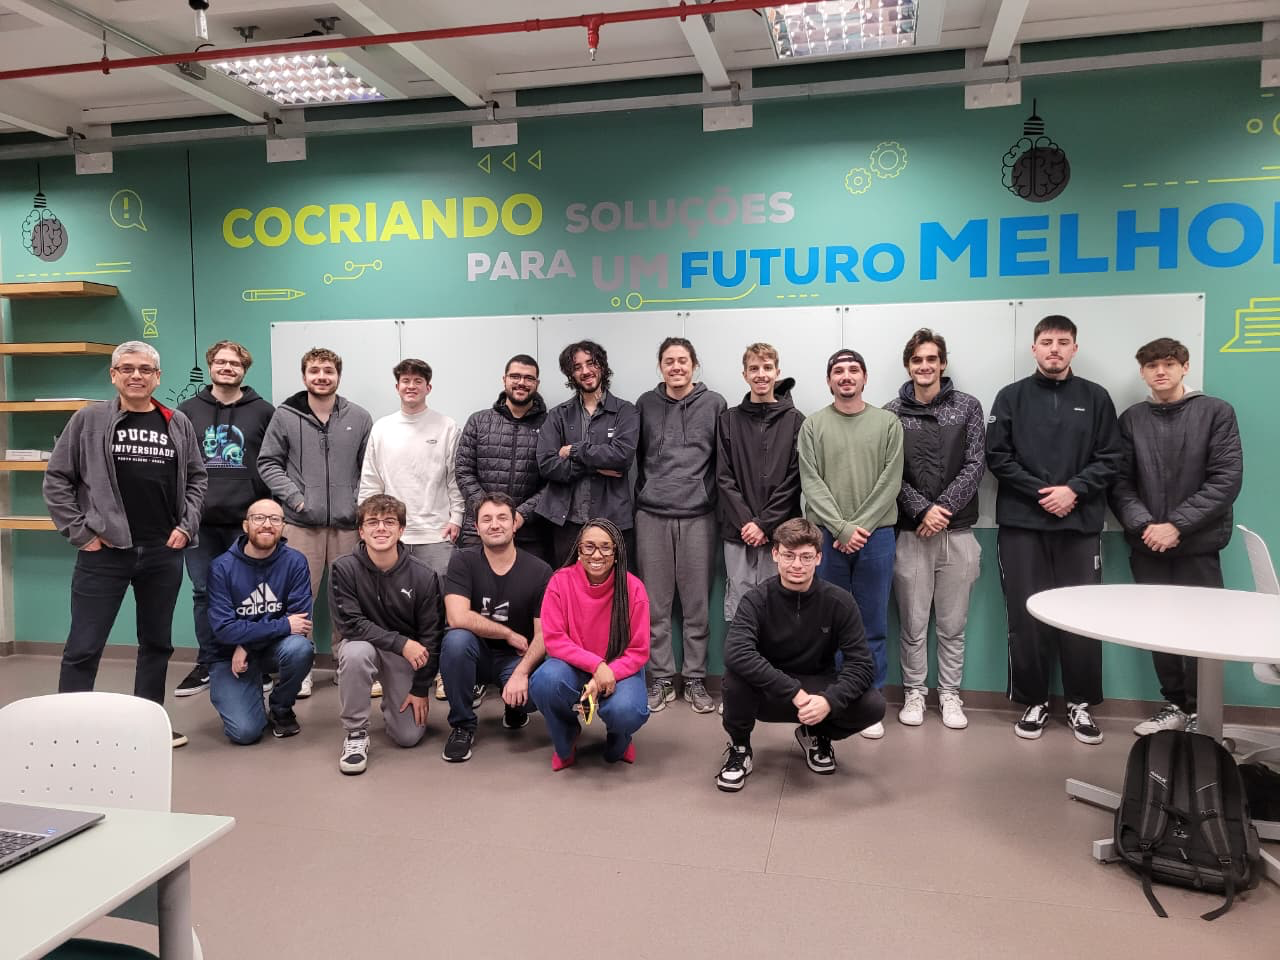
\includegraphics[width=0.9\linewidth,height=0.34\textheight,keepaspectratio]{conteudo/4 - ages III/conteudo/figures/equipe-vinculohub.png}
    \legend{Fonte: \href{https://tools.ages.pucrs.br/vinculo-hub/wiki/-/wikis/home}{wiki do projeto VínculoHub Portal}.}
\end{figure}

\section{Desenvolvimento do Projeto}

\subsection{Repositório do Código Fonte do Projeto}

O projeto \textbf{VínculoHub Portal} foi organizado em um repositório principal no GitHub, contendo as aplicações de \textit{frontend} e \textit{backend}, a documentação técnica, os arquivos de infraestrutura e os \textit{scripts} de apoio ao desenvolvimento.

\begin{itemize}
\item Repositório principal: \url{https://github.com/VinculoHub-Portal/VinculoHubPortal}
\end{itemize}

A estrutura do repositório foi dividida principalmente entre as pastas \texttt{frontend}, \texttt{backend} e \texttt{docs}. A pasta \texttt{frontend} concentrou a aplicação \textit{web} utilizada pelos diferentes perfis de usuário. A pasta \texttt{backend} reuniu a \ac{API}, as regras de negócio, a integração com banco de dados, autenticação, documentos e serviços externos. A pasta \texttt{docs} foi utilizada para registrar materiais de apoio, validações de \textit{sprint}, tarefas refinadas e a modelagem do banco de dados.

Além disso, o projeto possui arquivos de orquestração e infraestrutura, como \texttt{docker-compose.yml}, \texttt{docker-compose.dev.yml}, \texttt{docker-compose.swarm.yml} e \texttt{main.tf}, evidenciando uma preocupação com padronização de ambiente, execução local e preparação para \textit{deploy} em nuvem.

\subsection{Banco de Dados Utilizado}

O banco de dados utilizado no projeto foi o \textbf{PostgreSQL}. A aplicação também utilizou \textbf{Flyway} para versionamento e execução das migrações do banco, permitindo que a estrutura fosse reproduzida de forma consistente nos ambientes de desenvolvimento e \textit{deploy}.

A Figura~\ref{fig:vinculohub-banco-dados} apresenta a modelagem. O banco foi documentado em formato \ac{DBML} no arquivo \texttt{docs/db/vinculo\_hub.dbml}. Entre as principais entidades modeladas estão usuários, \ac{ONGs}, empresas, projetos, documentos, editais, \ac{ODS}, endereços, denúncias e vínculos entre empresas e projetos.

\begin{figure}[!htbp]
    \centering
    \small
    \caption{Modelagem do banco de dados do VínculoHub Portal}
    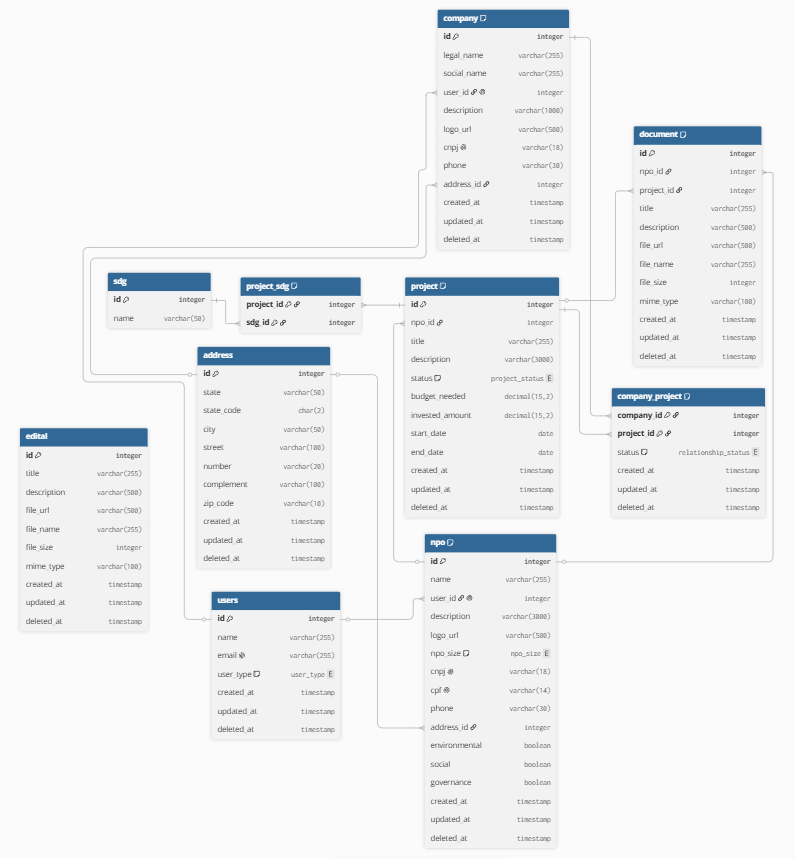
\includegraphics[width=1\linewidth]{conteudo/4 - ages III/conteudo/figures/banco-dados-vinculohub.png}
    \legend{Fonte: wiki do VínculoHub Portal \cite{vinculohub}.}
    \label{fig:vinculohub-banco-dados}
\end{figure}

A entidade \texttt{users} armazena os dados básicos do usuário e mantém integração com o Auth0 por meio do campo \texttt{auth0\_id}. As entidades \texttt{npo} e \texttt{company} representam, respectivamente, \ac{ONGs} e empresas cadastradas na plataforma. A entidade \texttt{project} centraliza os projetos cadastrados pelas \ac{ONGs}, enquanto \texttt{document} armazena metadados de arquivos vinculados a \ac{ONGs} ou projetos. A tabela \texttt{company\_project} representa os vínculos entre empresas e projetos, com status como pendente, em negociação, ativo ou inativo.

\subsection{Arquitetura Utilizada}

A Figura~\ref{fig:vinculohub-arquitetura} apresenta a infraestrutura documentada. A arquitetura do projeto foi baseada em uma aplicação \textit{web} separada em \textit{frontend}, \textit{backend}, banco de dados e serviços externos. O \textit{frontend} se comunica com o \textit{backend} por meio de \ac{API} \ac{REST}. O \textit{backend} centraliza as regras de negócio, validações, persistência dos dados, segurança e integrações externas. O banco PostgreSQL armazena os dados relacionais da aplicação.

A autenticação e autorização foram integradas ao \textbf{Auth0}, com separação de perfis por \textit{roles}, como \texttt{COMPANY}, \texttt{NPO} e \texttt{ADMIN}. Essa separação permitiu controlar o acesso às rotas e funcionalidades específicas de empresas, \ac{ONGs} e administradores.

O projeto também utilizou \textbf{Docker Compose} para execução local dos serviços, incluindo \textit{backend}, \textit{frontend}, banco PostgreSQL e Flyway. Para armazenamento de arquivos, como documentos e editais, foi prevista integração com \textbf{\ac{AWS} \ac{S3}}. A documentação e os arquivos de infraestrutura também indicam uma organização voltada a \textit{deploy} em ambiente \ac{AWS}, com uso de \ac{EC2}, Docker Swarm, Elastic Block Storage e \textit{bucket} \ac{S3}.

\begin{figure}[!htbp]
    \centering
    \small
    \caption{Arquitetura de infraestrutura do VínculoHub Portal}
    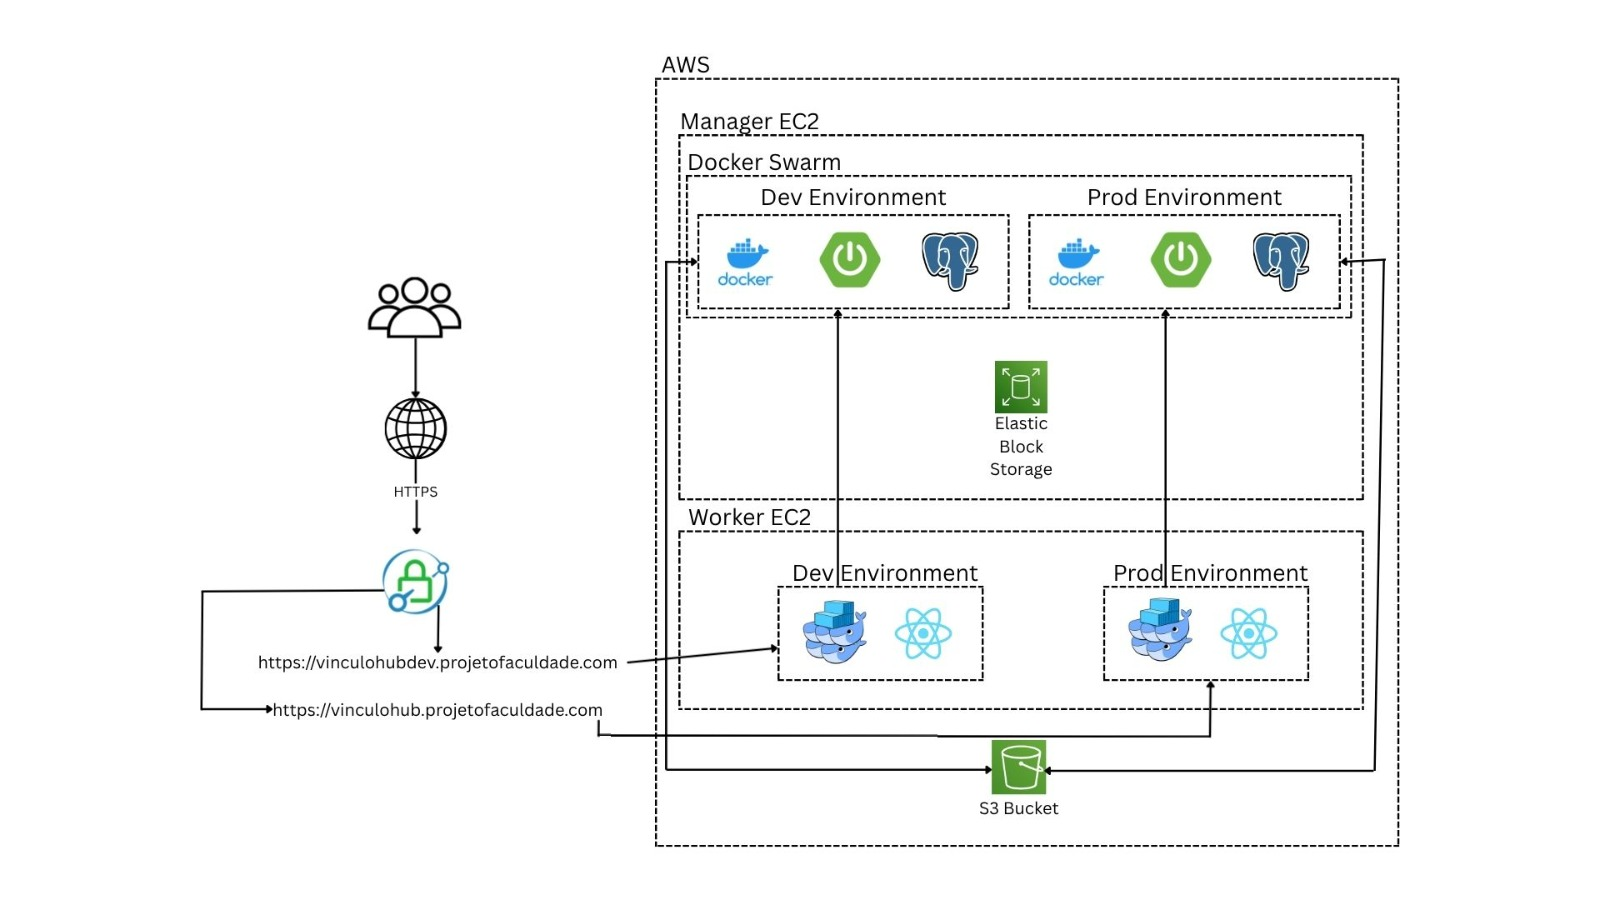
\includegraphics[width=1\linewidth]{conteudo/4 - ages III/conteudo/figures/arquitetura-vinculohub.jpeg}
    \legend{Fonte: wiki do VínculoHub Portal \cite{vinculohub}.}
    \label{fig:vinculohub-arquitetura}
\end{figure}

Essa arquitetura permitiu organizar ambientes de desenvolvimento e produção, padronizar a execução dos serviços e separar responsabilidades entre interface, \ac{API}, banco de dados, autenticação e armazenamento de arquivos.

\subsection{Protótipos das Telas Desenvolvidas}

Durante o desenvolvimento do VínculoHub Portal, os protótipos e fluxos de tela serviram como base para a construção das principais experiências da aplicação. Entre os fluxos contemplados estavam o cadastro de \ac{ONGs}, cadastro de empresas, \textit{dashboards} por perfil, mural de editais, perfil público de \ac{ONGs}, perfil público de empresas, cadastro e edição de projetos, \textit{upload} de documentos, denúncias e gestão de vínculos.

No \textit{frontend}, esses fluxos foram implementados em páginas e componentes específicos, como \texttt{AdminDashboard}, \texttt{CompanyDashboard}, \texttt{OngProfilePage}, \texttt{OngPublicProfilePage}, \texttt{ProjectDetailsPage}, \texttt{EditaisMuralPage}, \texttt{MyRelationshipsPage} e páginas administrativas para \ac{ONGs}, vínculos e notificações.

A documentação visual está disponível na \href{https://tools.ages.pucrs.br/vinculo-hub/wiki/-/wikis/home}{wiki do VínculoHub Portal}. A Figura~\ref{fig:vinculohub-painel} ilustra o painel de uma \ac{ONG} e sua organização em torno dos projetos, editais e vínculos. A tela ajuda a relacionar os fluxos descritos à proposta de aproximar organizações sociais e empresas.

\begin{figure}[htbp]
    \centering
    \caption{Painel de uma ONG no VínculoHub Portal}
    \label{fig:vinculohub-painel}
    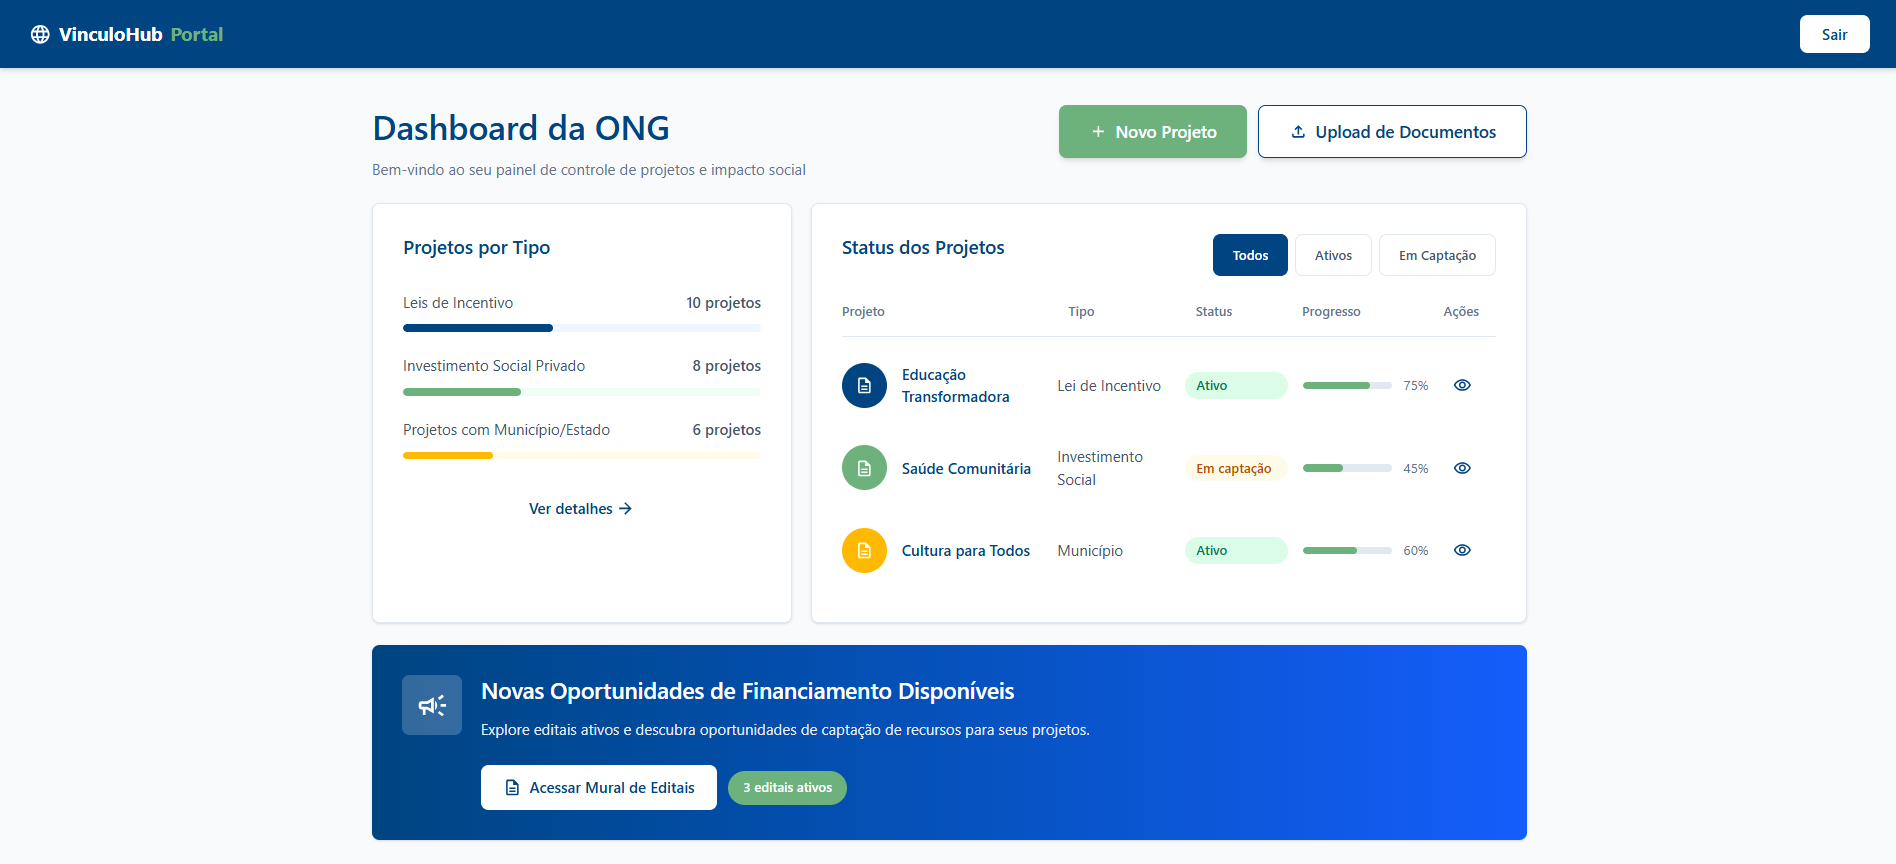
\includegraphics[width=\linewidth,height=0.36\textheight,keepaspectratio]{conteudo/4 - ages III/conteudo/figures/tela-painel-vinculohub.png}
    \legend{Fonte: wiki do VínculoHub Portal \cite{vinculohub}.}
\end{figure}

\subsection{Tecnologias Utilizadas}

No \textit{frontend}, React organizou a interface em componentes, TypeScript apoiou a verificação de tipos e Vite forneceu ferramentas de desenvolvimento e construção da aplicação. Material \ac{UI} ofereceu componentes de interface e Tailwind \ac{CSS} apoiou a estilização \cite{react,typescript,vite,mui,tailwind}.

React Router organizou a navegação; React Query apoiou a consulta e o gerenciamento de dados remotos; Axios foi utilizado nas requisições \ac{HTTP}. A integração de autenticação foi apoiada pelo \ac{SDK} do Auth0. Para a qualidade da interface, Vitest foi empregado na execução de testes, Testing Library na verificação de componentes e Playwright em cenários de ponta a ponta \cite{router,query,axios,auth0,vitest,testinglibrary,playwright}.

No \textit{backend}, Java 17 e Spring Boot sustentaram a \ac{API} e as regras de negócio. Os módulos Spring \textit{Web}, Spring Data \ac{JPA} e Spring Security apoiaram, respectivamente, os \textit{endpoints}, a persistência e a segurança, incluindo a validação de acesso com OAuth2. PostgreSQL armazenou os dados e Flyway controlou as migrações. Lombok foi utilizado para reduzir código repetitivo, e Swagger/OpenAPI para a documentação das operações \cite{spring,jpa,security,postgres,flyway,lombok,vinculohub}.

Na infraestrutura, Docker e Docker Compose padronizaram a execução dos serviços. Os arquivos Terraform descreveram recursos de infraestrutura, enquanto os serviços \ac{AWS} foram utilizados no contexto de implantação e armazenamento, incluindo \ac{S3} para documentos \cite{docker,terraform,aws}.

Na qualidade do \textit{backend}, o projeto utilizou JUnit para testes, Testcontainers para dependências em ambiente isolado e JaCoCo para cobertura, conforme o registro técnico do projeto. Spotless apoiou a formatação; PMD e SpotBugs realizaram análise estática. Sua presença não comprova a validação de todos os cenários \cite{junit,testcontainers,jacoco,spotless,pmd,spotbugs,vinculohub}.

\clearpage
\section{Atividades Desempenhadas pelo Aluno}


\subsection{Sprint 0}

No cronograma do semestre, a apresentação da \ac{AGES} e a integração das equipes estavam previstas para 2 de março de 2026, e a apresentação do projeto pelos \textit{stakeholders}, para 9 de março. A apresentação das histórias de usuário e dos \textit{mockups} e o planejamento da \textit{Sprint} 1 estavam marcados para 25 de março, seguidos da retrospectiva e do relatório da \textit{Sprint} 0 em 30 de março.

A \textit{Sprint} 0 teve papel decisivo para o sucesso inicial do projeto, pois concentrou toda a etapa de estruturação conceitual, definição visual e preparação organizacional da equipe. Diferentemente de fases iniciais em que normalmente há menor intensidade técnica, nesta oportunidade o volume de trabalho foi elevado desde os primeiros encontros, especialmente pela necessidade de transformar uma ideia ampla em um produto viável e bem organizado.

Minha atuação concentrou-se principalmente na frente de produto, experiência do usuário e organização das entregas. Auxiliei diretamente colegas da \ac{AGES} I no desenvolvimento dos \textit{mockups}, esclarecendo dúvidas sobre boas práticas de interface, padronização visual e coerência entre telas. Busquei contribuir não apenas executando tarefas, mas também orientando membros menos experientes, compartilhando conhecimentos adquiridos em experiências anteriores e no ambiente profissional.

Participei ativamente da definição dos fluxos centrais da aplicação. Como o sistema possuía múltiplos perfis de usuários --- \ac{ONGs}, empresas investidoras e administradores --- foi necessário pensar cuidadosamente na jornada de cada tipo de usuário dentro da plataforma. Assim, colaborei na concepção lógica dos seguintes fluxos:

\begin{itemize}
\item cadastro institucional de \ac{ONGs};
\item cadastro empresarial;
\item portal administrativo;
\item listagem e gerenciamento de projetos;
\item sistema de vínculos entre organizações e empresas;
\item mural de editais;
\item denúncias de irregularidades;
\item edição de perfis institucionais;
\item visualização pública e privada de perfis.
\end{itemize}

Além disso, realizei \textit{benchmarking} de plataformas já consolidadas no mercado, analisando soluções semelhantes para identificar padrões modernos de navegação, \textit{layout}, \textit{onboarding} e \textit{dashboards}. Essa etapa foi importante para evitar decisões arbitrárias e elevar o nível de maturidade visual do produto.

Também participei da criação e refinamento de tarefas no Kanban, ajudando a transformar ideias amplas em demandas executáveis e priorizadas. Em diversos momentos, alinhei expectativas com colegas da \ac{AGES} IV sobre escopo, prioridades e viabilidade de determinadas funcionalidades.

Durante essa \textit{sprint}, percebi claramente a importância da comunicação em projetos colaborativos. Como havia muitas ideias simultâneas e diferentes níveis de experiência entre os integrantes, nem sempre o fluxo de informação acontecia da melhor forma. Isso exigiu postura mais ativa da minha parte, buscando centralizar dúvidas, destravar tarefas e orientar colegas.

Considero que a \textit{Sprint} 0 foi extremamente produtiva para mim, pois atuei em áreas diversas: \ac{UX}, produto, organização ágil e apoio técnico ao time. Também serviu para consolidar uma postura mais madura de liderança informal, auxiliando colegas e pensando no projeto de forma sistêmica, não apenas individual.

\vspace{0.5cm}

\clearpage
\subsection{Sprint 1}

O cronograma previa a apresentação da \textit{Sprint} 1 aos \textit{stakeholders} e o planejamento da \textit{Sprint} 2 em 15 de abril de 2026. A retrospectiva, o relatório da \textit{sprint} e o Relatório de Acompanhamento no formato de memorial estavam previstos para 22 de abril. Essas datas situam os marcos de planejamento da etapa.

Após a estruturação e a prototipação da \textit{Sprint} 0, passamos a implementar a base funcional da plataforma. Minha principal atuação concentrou-se na autenticação e no controle de acesso. Como o sistema possuía perfis distintos de organizações sociais, empresas e administradores, essa base precisava considerar as diferentes jornadas e permissões.

Estudei provedores de autenticação externa, entre eles Clerk, Firebase e Auth0. Consultei a documentação e discuti com os colegas as possibilidades de integração e a adequação ao projeto. Optamos pelo Auth0, considerando os recursos de perfis de acesso e sua integração com as aplicações. Em seguida, participei da configuração inicial e da conexão com o sistema.

Esse trabalho envolveu a criação e configuração do ambiente da aplicação no provedor, a definição de perfis e permissões, usuários de teste e redirecionamentos após o acesso. Também participei da integração do \textit{frontend}, da validação dos \textit{tokens} no \textit{backend} e da sincronização das identidades externas com os registros internos. No banco, contribuí para a inclusão do campo \texttt{auth0\_id} na tabela de usuários, estabelecendo a associação com o Auth0, além de ajustes de nomenclatura e padronização.

Paralelamente, participei dos \textit{squads} criados para dividir o trabalho. Essa organização ajudou a concentrar responsabilidades, mas percebi dificuldades de alinhamento, atrasos e tarefas executadas perto do prazo. Mesmo sem ocupar uma posição formal de liderança, reconheci que poderia ter acompanhado melhor as dependências e comunicado os riscos mais cedo. O conhecimento técnico que eu já possuía não eliminava a necessidade de atenção à organização coletiva.

Ao final, avançamos na autenticação, na definição de perfis e na integração entre as camadas. Ficou pendente a tela de cadastro do primeiro projeto da \ac{ONG}, que fazia parte do fluxo de entrada da organização na plataforma. Essa etapa era importante para que o cadastro institucional estivesse acompanhado de uma iniciativa concreta a ser apresentada às empresas.

A pendência envolvia dependências entre interface, persistência de projetos, autenticação e coerência visual com as demais etapas do cadastro. As tarefas próximas do prazo reduziram o tempo para revisão, integração e correções. Essa situação mostrou que uma tela aparentemente localizada podia exigir coordenação entre várias partes do sistema. Também reforçou a necessidade de manter o diálogo entre prototipação e implementação durante a \textit{sprint}.

Minha principal autocrítica foi não ter antecipado suficientemente os gargalos do \textit{squad}. Eu poderia ter buscado alinhamentos mais frequentes e sinalizado as dificuldades antes de se acumularem. O aprendizado foi reconhecer a diferença entre concluir uma implementação e concluir um fluxo utilizável: a entrega depende das integrações, da revisão e da clareza sobre o que permanece pendente. A base de autenticação avançou, mas o cadastro do primeiro projeto ainda precisava ser finalizado.

\clearpage
\subsection{Sprint 2}

A apresentação da \textit{Sprint} 2 e o planejamento da \textit{Sprint} 3 estavam previstos para 6 de maio de 2026, com retrospectiva e entrega do relatório em 11 de maio. O cronograma também reservava encontros anteriores ao desenvolvimento e a reuniões individuais de acompanhamento.

A \textit{Sprint} 2 teve como foco avançar na experiência de uso dos dois perfis centrais da plataforma: \ac{ONGs} e empresas. As atividades previstas estavam concentradas principalmente no \textit{frontend}, com a entrega da visualização principal dos projetos da \ac{ONG} e a construção da vitrine de busca e modalidades de investimento para empresas. A primeira frente tinha como objetivo permitir que a \ac{ONG} acompanhasse rapidamente seus projetos, visualizando informações relevantes sem precisar navegar por fluxos excessivamente longos. A segunda frente buscava melhorar a descoberta de oportunidades por parte das empresas, aproximando-as de projetos alinhados aos seus interesses.

Todas as atividades previstas para a \textit{sprint} foram concluídas. Do ponto de vista do produto, essa etapa foi importante porque começou a tornar a plataforma mais utilizável para os perfis finais. Até então, boa parte do esforço estava concentrada na estruturação da base do sistema, autenticação, modelagem e fluxos iniciais. Na \textit{Sprint} 2, o projeto passou a ganhar mais corpo visual e funcional, especialmente na experiência de navegação das \ac{ONGs} e das empresas.

Minha atuação esteve relacionada ao acompanhamento das demandas do \textit{squad}, ao entendimento das entregas previstas e ao apoio na organização das atividades de \textit{frontend}. Como eu já possuía mais experiência do que em \ac{AGES} anteriores, passei a perceber com mais clareza os impactos de uma história de usuário mal definida ou de uma divisão de responsabilidades pouco explícita. Esse foi justamente um dos principais problemas encontrados durante a \textit{sprint}.

A maior dificuldade foi a falta de clareza nas histórias de usuário e nas funções de cada \textit{squad}. No início, entendíamos que o nosso \textit{squad}, chamado de User Experience, teria como responsabilidade principal concluir tarefas relacionadas ao \textit{frontend}. Entretanto, ao longo da \textit{sprint}, ficou claro que a expectativa não era apenas implementar telas, mas também pensar fluxo, experiência, coerência do produto, alinhamento com regras de negócio e comunicação com outros \textit{squads}. Essa diferença de entendimento gerou ruídos, pois algumas tarefas pareciam pertencer a uma frente, mas dependiam diretamente de decisões ou entregas de outra.

Esse problema evidenciou uma fragilidade importante na comunicação entre \ac{AGES} III e \ac{AGES} IV. Como os integrantes da \ac{AGES} III estavam em posição de maior responsabilidade na gestão dos \textit{squads}, era esperado que tivéssemos uma postura mais ativa na interpretação das demandas, na divisão das tarefas e na comunicação com os demais membros. No entanto, percebi que ainda havia dificuldade em transformar decisões de alto nível em tarefas claras para execução.

A principal lição aprendida foi que a comunicação entre \ac{AGES} III e \ac{AGES} IV precisava melhorar, especialmente porque os \ac{AGES} III estavam cada vez mais envolvidos na gestão dos \textit{squads}. Liderar tecnicamente ou organizar um grupo não significa apenas distribuir tarefas, mas garantir que todos entendam o propósito da entrega, os critérios de aceite e as dependências envolvidas. Quando esse alinhamento não acontece, mesmo tarefas aparentemente simples podem gerar retrabalho ou insegurança na equipe.

Como próximo passo, entendi que seria necessário desenvolver o projeto de forma mais próxima dos \ac{AGES} IV, buscando validar expectativas com antecedência e reduzir ambiguidades. Essa \textit{sprint} reforçou que, em projetos colaborativos, a qualidade da entrega depende tanto da implementação quanto da clareza do processo que leva até ela.

\clearpage
\subsection{Sprint 3}

No cronograma, a apresentação da \textit{Sprint} 3 aos \textit{stakeholders} e o planejamento da \textit{Sprint} 4 estavam marcados para 1º de junho de 2026. A retrospectiva e a entrega do relatório dessa etapa estavam previstas para 3 de junho.

A \textit{Sprint} 3 concentrou um conjunto mais amplo de funcionalidades e melhorias na plataforma. As atividades previstas incluíam o aprimoramento da tela de detalhe dos projetos, o \textit{dashboard} de indicadores de impacto da \ac{ONG}, a edição de projetos, a história de usuário de visibilidade e acesso ao perfil da \ac{ONG}, além do \textit{upload} e visualização de documentos institucionais. Todas as atividades previstas foram concluídas, o que representou um avanço importante na maturidade do produto.

Essa \textit{sprint} exigiu maior articulação entre \textit{frontend}, \textit{backend}, validações de negócio e experiência do usuário. Diferentemente de tarefas isoladas de interface, as funcionalidades previstas dependiam de dados reais, regras de acesso, integração com autenticação e comportamento coerente entre diferentes páginas. Por isso, minha atuação foi se deslocando cada vez mais para atividades de análise, apoio técnico, revisão e organização do trabalho do \textit{squad}.

No início da \textit{sprint}, dediquei tempo ao estudo do estado atual do \textit{backend} e à criação de \textit{subtasks} referentes a essa camada. Esse trabalho foi importante para transformar demandas amplas em tarefas menores e mais executáveis. Também participei de \textit{weeklys} e sugeri a criação de uma nova tabela no banco de dados, a partir das necessidades percebidas durante o desenvolvimento. Além disso, revisei \textit{pull requests} relacionados à edição de \ac{ONGs}, alinhei decisões com integrantes da \ac{AGES} III do \textit{squad} e busquei entender melhor a construção dos processos de tratamento e processamento de documentos no \textit{backend}.

Uma das atividades mais relevantes foi auxiliar um colega do \textit{squad} na configuração da geração de \textit{tokens} do Auth0 no Postman. Esse tipo de apoio foi importante porque a autenticação era uma parte central do projeto e, sem conseguir simular corretamente os perfis e permissões, o desenvolvimento e os testes ficavam travados. Esse momento reforçou a importância de dominar não apenas o código da funcionalidade, mas também o ambiente necessário para que os colegas consigam trabalhar.

Mais adiante, atuei na revisão de \textit{pull requests}, no apoio a colegas com erros e na implementação da história de usuário de listagem e \textit{download} de documentos. Essa funcionalidade dialogava diretamente com uma necessidade importante das \ac{ONGs}: armazenar e disponibilizar documentos institucionais de forma organizada e segura. Ao trabalhar nessa frente, precisei considerar aspectos de \textit{frontend}, \textit{endpoints}, permissões e experiência de uso, principalmente para garantir que os documentos fossem exibidos de forma compreensível e pudessem ser acessados quando necessário.

Apesar de as entregas terem sido concluídas, o principal problema encontrado foi a gestão de pessoas. A \textit{sprint} deixou claro que, conforme o projeto cresce, o desafio deixa de ser apenas técnico. A coordenação entre pessoas, expectativas, ritmos de trabalho e responsabilidades passa a ocupar um papel central. Em alguns momentos, percebi dificuldade em manter todos alinhados, tanto dentro do \textit{squad} quanto com pessoas de fora dele.

A principal lição aprendida foi a necessidade de melhorar o canal de comunicação entre os membros do \textit{squad} e também com outros \textit{squads}. A falta de comunicação clara não gera apenas atraso; ela cria insegurança, sobreposição de tarefas e perda de contexto. Para um projeto com múltiplos perfis, muitas funcionalidades e diferentes níveis de experiência entre os integrantes, esse alinhamento precisa ser constante.

Ao final da \textit{sprint}, o \textit{squad} ficou com tarefas de refatoração e limpeza do código. Esse próximo passo foi importante porque, após várias entregas funcionais, tornou-se necessário melhorar a organização interna da aplicação, reduzir inconsistências e preparar o projeto para as etapas finais. Para mim, a \textit{Sprint} 3 foi uma fase de aprendizado mais voltada à sustentação de um projeto em crescimento, especialmente na relação entre apoio técnico, revisão de código, comunicação e gestão de pessoas.

\clearpage
\subsection{Sprint 4}

O cronograma previa a entrega final do projeto, a retrospectiva e o relatório da \textit{Sprint} 4 em 22 de junho de 2026. Em 24 de junho, estavam previstas a retrospectiva geral da \ac{AGES} e a entrega do memorial final; a apresentação dos projetos para os demais times estava marcada para 29 de junho. Esses marcos de programação não substituem o relato do estado efetivo da aplicação na entrega.

A \textit{Sprint} 4 representou a etapa final de consolidação do projeto. As atividades previstas envolviam o card de projetos apoiados no \textit{dashboard} da empresa, a criação da tela de notificações no painel dos administradores, a criação do perfil da empresa e a remoção dos \textit{mocks} restantes do CompanyDashboard. Todas as atividades previstas foram concluídas, o que ajudou a aproximar o sistema de um estado mais consistente para apresentação e validação final.

Nesta \textit{sprint}, minha atuação esteve bastante relacionada a revisão, planejamento e implementação de ajustes no painel administrativo. Participei da contabilização das horas da \textit{weekly} de sábado, revisei \textit{pull requests} e ajudei colegas com erros encontrados durante o desenvolvimento. Também trabalhei no planejamento e implementação de um débito técnico no painel dos administradores, buscando reduzir inconsistências e tornar essa área mais coerente com as funcionalidades reais do sistema.

Uma das principais frentes em que atuei foi a criação do planejamento de implementação da listagem de notificações no painel de admin. Para isso, realizei uma varredura do painel administrativo, listei inconsistências de design, participei da \textit{weekly} e alinhei decisões com integrantes da \ac{AGES} III e IV. Em seguida, contribuí para a implementação da listagem de notificações, conectando essa necessidade ao fluxo de mediação e acompanhamento de vínculos dentro da plataforma.

A \textit{sprint} também envolveu melhorias importantes no \textit{dashboard} da empresa. A remoção de \textit{mocks} restantes do CompanyDashboard foi relevante porque aproximou a aplicação de um comportamento real, baseado em dados do \textit{backend}. O card de projetos apoiados também contribuiu para tornar a experiência da empresa mais útil, permitindo visualizar de forma mais direta os projetos vinculados e a divisão entre modalidades de investimento.

Apesar das entregas concluídas, o maior problema encontrado foi a falta de motivação e engajamento da equipe de desenvolvimento. Ao final do projeto, ficou perceptível que parte do time já demonstrava menor energia para continuar evoluindo a aplicação. Esse desgaste pode ser explicado por diversos fatores, como fim de semestre, acúmulo de demandas, complexidade do projeto e perda gradual de interesse pelo produto.

No meu caso, essa \textit{sprint} também evidenciou uma redução da minha própria presença no projeto. Eu ainda contribuía por meio de revisão, planejamento, apoio e implementação pontual, mas já não tinha o mesmo nível de envolvimento das fases iniciais. Essa redução não ocorreu por uma dificuldade técnica específica, mas por uma combinação de menor interesse pessoal pelo domínio de negócio do projeto e pela sensação de que eu já não estava aprendendo tantas coisas novas quanto em experiências anteriores.

A principal lição aprendida foi que a escolha de projetos deve considerar também preferências pessoais e interesse pelo domínio de negócio. Durante muito tempo, eu avaliei projetos principalmente pela stack ou pelo desafio técnico. No entanto, a \textit{Sprint} 4 deixou claro que o domínio de negócio precisa despertar algum nível de curiosidade nos desenvolvedores, principalmente quando o projeto entra em fases menos empolgantes, como ajustes, revisões e correções. Quando não existe conexão com o problema que está sendo resolvido, manter o engajamento se torna mais difícil.

Como próximos passos, o projeto ainda demandava ajustes no \textit{deploy} da aplicação. A infraestrutura já possuía uma base organizada, com Docker, \ac{AWS} e separação de ambientes, mas ainda havia necessidade de estabilizar e ajustar pontos finais para garantir uma entrega mais confiável. Para mim, essa \textit{sprint} encerrou a \ac{AGES} III com uma reflexão importante: maturidade técnica não depende apenas de saber implementar, mas também de entender quais tipos de problema realmente despertam interesse e sustentam participação ao longo do tempo.


\section{Conclusão}

A AGES III ocorreu em um momento em que eu já tinha mais segurança técnica e experiência profissional. No VínculoHub Portal, isso ampliou minha participação em decisões de produto, autenticação, organização de tarefas, revisão de código e apoio aos colegas. Ao mesmo tempo, passei a perceber com mais clareza problemas de comunicação e de alinhamento entre os \textit{squads}.

Minha participação foi mais intensa nas etapas iniciais. Com o avanço do semestre, percebi uma redução do meu engajamento, relacionada ao menor interesse pessoal pelo domínio de negócio e à sensação de encontrar menos aprendizados técnicos novos nas tarefas de ajuste e revisão. Reconheço o valor social da proposta, mas esse reconhecimento não se traduziu, em todos os momentos, na mesma disposição para acompanhar o projeto. Essa foi uma autocrítica importante: eu precisava sustentar minha responsabilidade também nas etapas de correção e consolidação.

Do ponto de vista técnico, aprofundei o contato com autenticação, integração entre camadas, banco de dados e revisão das implementações. A organização de subtarefas e o acompanhamento dos \textit{squads} se relacionaram aos conhecimentos de Processos de Software e Gerenciamento de Projetos de Software. A leitura da arquitetura e das integrações também aproximou a prática de Projeto e Arquitetura de Software, especialmente quando precisei entender uma demanda antes de distribuí-la ou revisar o código correspondente.

Na comunicação, histórias de usuário pouco claras, responsabilidades ambíguas e tarefas próximas do prazo evidenciaram pontos que poderiam ter sido tratados mais cedo. Eu poderia ter sido mais proativo no acompanhamento das dependências e no esclarecimento de dúvidas. O apoio aos colegas e a divisão em \textit{squads} foram positivos, mas exigiam alinhamento contínuo para produzir o resultado esperado.

O projeto também me ajudou a reconhecer a importância do interesse pelo problema de negócio na escolha das experiências profissionais. Passei a considerar, além da tecnologia, minha disposição para compreender o produto e acompanhar sua evolução. Com o uso mais frequente de agentes de inteligência artificial, essa percepção ganhou espaço na minha forma de trabalhar: fornecer contexto e revisar uma solução exigia entender o que precisava ser construído e por quê.

O VínculoHub ampliou minha compreensão sobre organização, comunicação e envolvimento com o domínio de negócio. Na comparação pessoal entre os quatro projetos, considero o ReadRace a melhor experiência, sobretudo pelo aprendizado em gestão e pela evolução pessoal alcançada na AGES IV. A AGES III contribuiu para esse percurso ao tornar mais visíveis tanto minhas capacidades quanto os pontos em que eu precisava melhorar.



\chapter[AGES IV --- ReadRace]{AGES IV --- ReadRace}
\section{Introdução}

Na AGES IV, no segundo semestre de 2026, passei a integrar o projeto ReadRace, sob orientação do professor Gabriel Fonseca Silva. O projeto propõe um aplicativo mobile para incentivar o hábito da leitura por meio de biblioteca pessoal, acompanhamento de progresso, interação social e gamificação. Seus stakeholders são Bernardo Schedler, Gabriela de Moraes, José Pedro Schury e Monique Soares Silveira.

O problema apresentado pelos clientes envolveu a dificuldade de manter a constância na leitura diante das distrações digitais. A proposta foi tornar esse hábito mais estimulante por meio de metas, desafios e recompensas. No refinamento do escopo, a equipe adotou como princípio valorizar o progresso sem punir os períodos de ausência. A leitura dos livros ocorre fora da plataforma: o aplicativo acompanha a atividade do leitor, sem hospedar o conteúdo das obras. Pagamentos e monetização ficaram fora do escopo.

Nesta etapa, minha atuação passou a envolver mais diretamente a gestão do projeto, em conjunto com os demais colegas de AGES IV. Participei de alinhamentos, preparação de perguntas aos clientes, discussão de user stories, revisão da modelagem de dados, acompanhamento de tarefas e apresentações. Também contribuí com o desenvolvimento e a revisão de código do projeto.

A equipe do ReadRace é apresentada na Figura~\ref{fig:readrace-equipe}. O projeto reuniu alunos de diferentes níveis da AGES, exigindo comunicação entre as responsabilidades de gestão, arquitetura, banco de dados e desenvolvimento.

\begin{figure}[H]
    \centering
    \caption{Equipe do projeto ReadRace}
    \label{fig:readrace-equipe}
    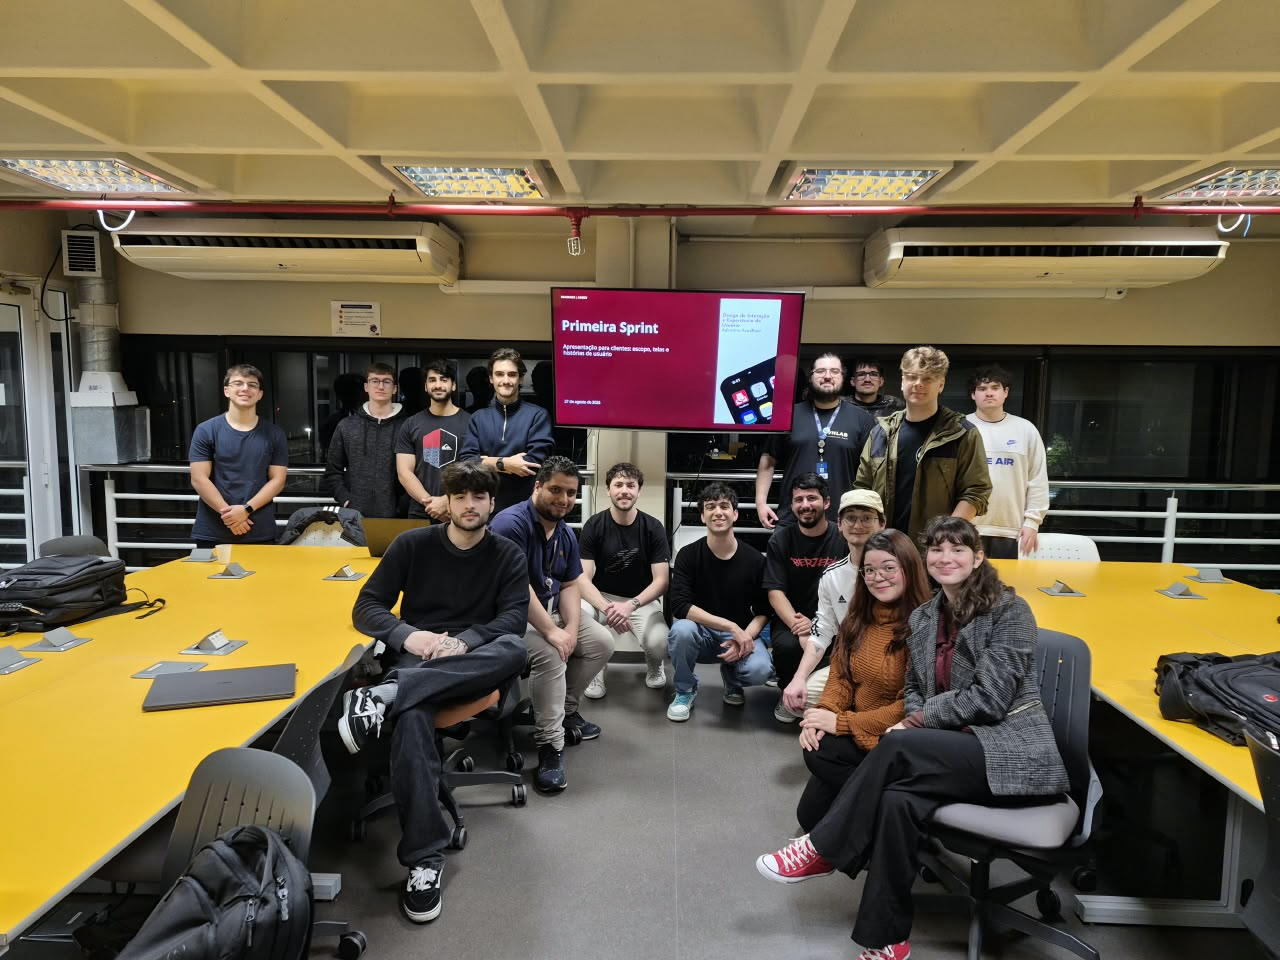
\includegraphics[width=0.9\linewidth,height=0.34\textheight,keepaspectratio]{conteudo/5 - ages IV/conteudo/figures/equipe-readrace.jpeg}
    \legend{Fonte: \href{https://tools.ages.pucrs.br/2026-2/6lmnp/readrace/readrace-wiki/-/wikis/home}{wiki do projeto ReadRace}.}
\end{figure}

\section{Desenvolvimento do Projeto}

\subsection{Repositório do Código Fonte do Projeto}

O código está disponível em \url{https://github.com/ReadRace-AGES/ReadRace}. O projeto utiliza um monorepositório com as pastas \texttt{backend} e \texttt{mobile}, tendo \texttt{dev} como branch principal de desenvolvimento. As tarefas são acompanhadas em \url{https://github.com/orgs/ReadRace-AGES/projects/1}. A wiki institucional reúne escopo, configuração e arquitetura: \url{https://tools.ages.pucrs.br/2026-2/6lmnp/readrace/readrace-wiki/-/wikis/home}.

O repositório de gestão AGESIV reúne os requisitos, as decisões de produto e o planejamento das sprints, incluindo as dependências entre as tarefas.

\subsection{Banco de Dados Utilizado}

O sistema utiliza PostgreSQL 16, com alterações estruturais versionadas por migrations do Flyway. O Hibernate valida o schema, enquanto as migrations são responsáveis por sua evolução. O modelo relacional em DBML, versão 8, contempla usuários, livros, autores, gêneros, itens da biblioteca e registros de leitura, além de entidades sociais e de gamificação.

Entre os relacionamentos estão os vínculos entre livros e autores, a associação dos livros à biblioteca de cada usuário, a participação em clubes e comunidades, os desafios entre amigos e as conquistas.

A revisão da coerência entre esse modelo e as user stories foi uma das minhas contribuições. Identifiquei divergências, registrei dúvidas e discuti sugestões com os demais AGES IV para alinhamento com os colegas responsáveis pela modelagem.

A Figura~\ref{fig:readrace-banco-dados} apresenta uma visão geral do modelo relacional disponível na wiki. A associação entre biblioteca, registros de leitura e recursos sociais permite compreender como o acompanhamento individual se relaciona às demais funcionalidades do aplicativo. O diagrama retrata a versão consultada na documentação, sem representar necessariamente o estado do banco na Sprint 1.

\begin{figure}[H]
    \centering
    \caption{Visão geral do modelo relacional do ReadRace}
    \label{fig:readrace-banco-dados}
    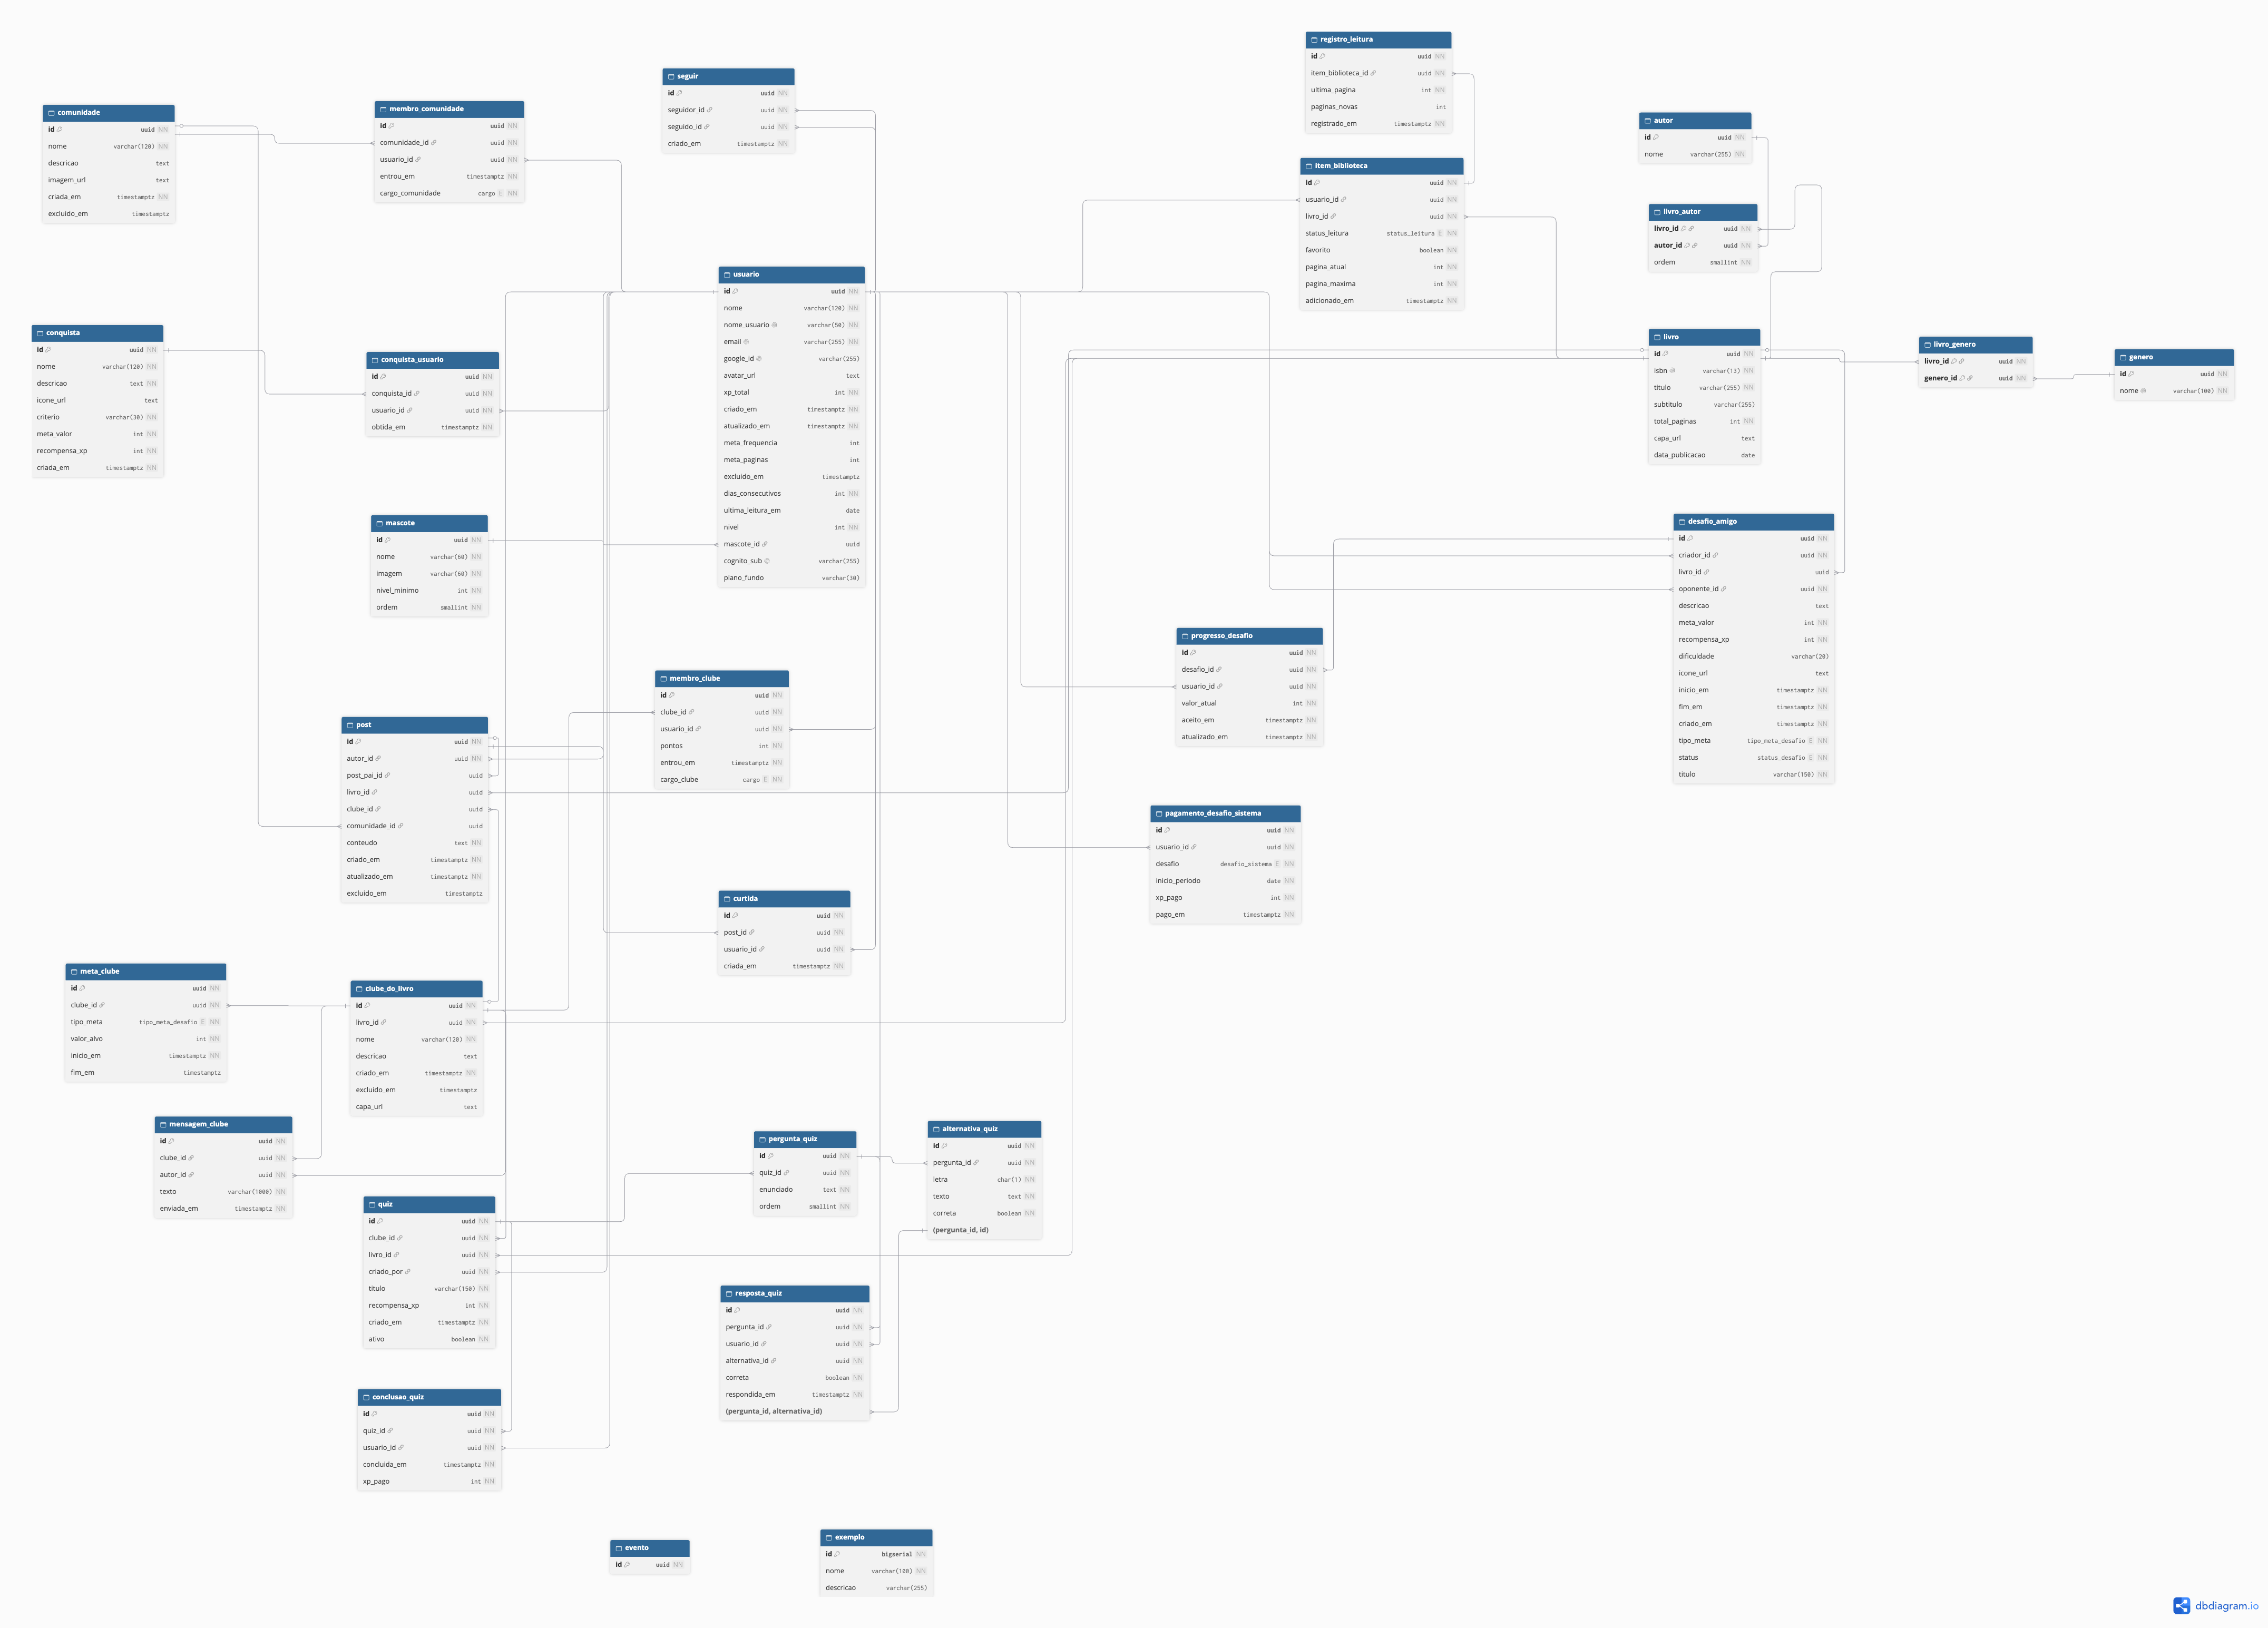
\includegraphics[width=\linewidth,height=0.56\textheight,keepaspectratio]{conteudo/5 - ages IV/conteudo/figures/banco-dados-readrace.png}
    \legend{Fonte: \href{https://tools.ages.pucrs.br/2026-2/6lmnp/readrace/readrace-wiki/-/wikis/banco-de-dados}{wiki do projeto ReadRace}.}
\end{figure}

\subsection{Arquitetura Utilizada}

O aplicativo mobile comunica-se com uma API Spring Boot, que concentra as regras de negócio e o acesso ao PostgreSQL. O backend organiza suas responsabilidades em Controller, Service e Repository. Para a consulta ao catálogo externo de livros, a documentação descreve uma interface com adaptadores: uma base local atende desenvolvimento e testes, enquanto a integração com Google Books é selecionada em produção.

No mobile, o expo-router organiza as rotas e as telas são agrupadas por funcionalidades. O tema e os componentes compartilhados favorecem a consistência da interface. Na Sprint 1, utilizamos um usuário fixo dos dados iniciais, identificado pelo backend.

\begin{figure}[H]
\centering
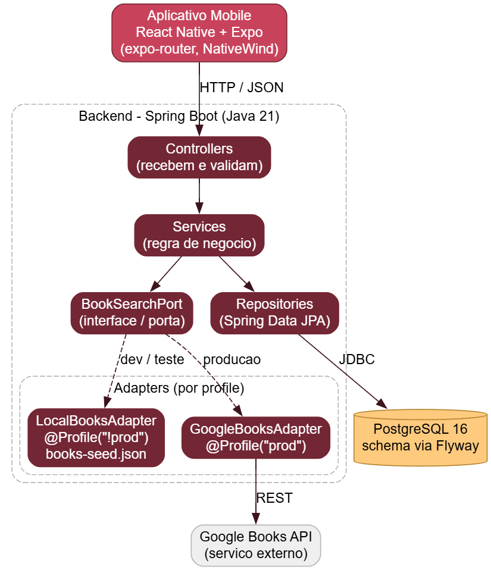
\includegraphics[width=\linewidth,height=0.42\textheight,keepaspectratio]{conteudo/5 - ages IV/conteudo/figures/arquitetura.png}
\caption{Arquitetura de aplicação do ReadRace.}
\legend{Fonte: wiki do projeto ReadRace.}
\end{figure}

A arquitetura de implantação descrita na wiki inclui Docker, NGINX, Cloudflare e serviços AWS, como EC2, ECR e SSM Parameter Store.

\subsection{Protótipos das Telas Desenvolvidas}

Os protótipos foram elaborados no Figma: \url{https://www.figma.com/design/N5iThb17TAP2AOIZWBt2zK/ReadRace}. O planejamento das telas contemplou biblioteca, detalhe do livro, registro de progresso, comunidades, clubes, fórum, busca, perfil público e desafios entre amigos.

\begin{figure}[H]
\centering
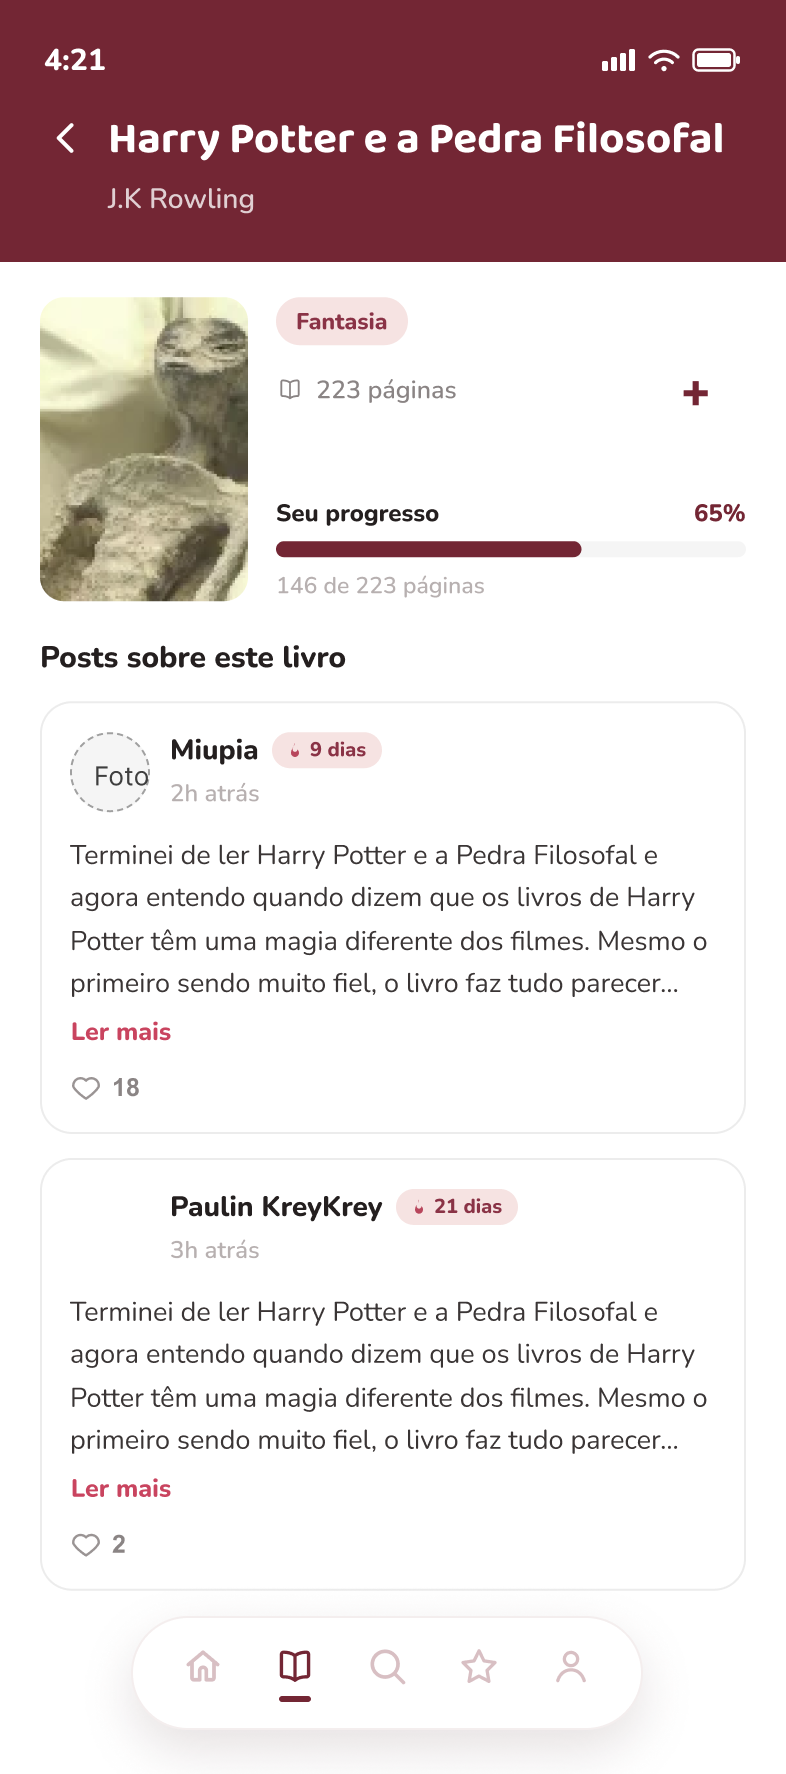
\includegraphics[width=0.43\linewidth,height=0.45\textheight,keepaspectratio]{conteudo/5 - ages IV/conteudo/figures/detalhe-livro.png}
\hspace{1cm}
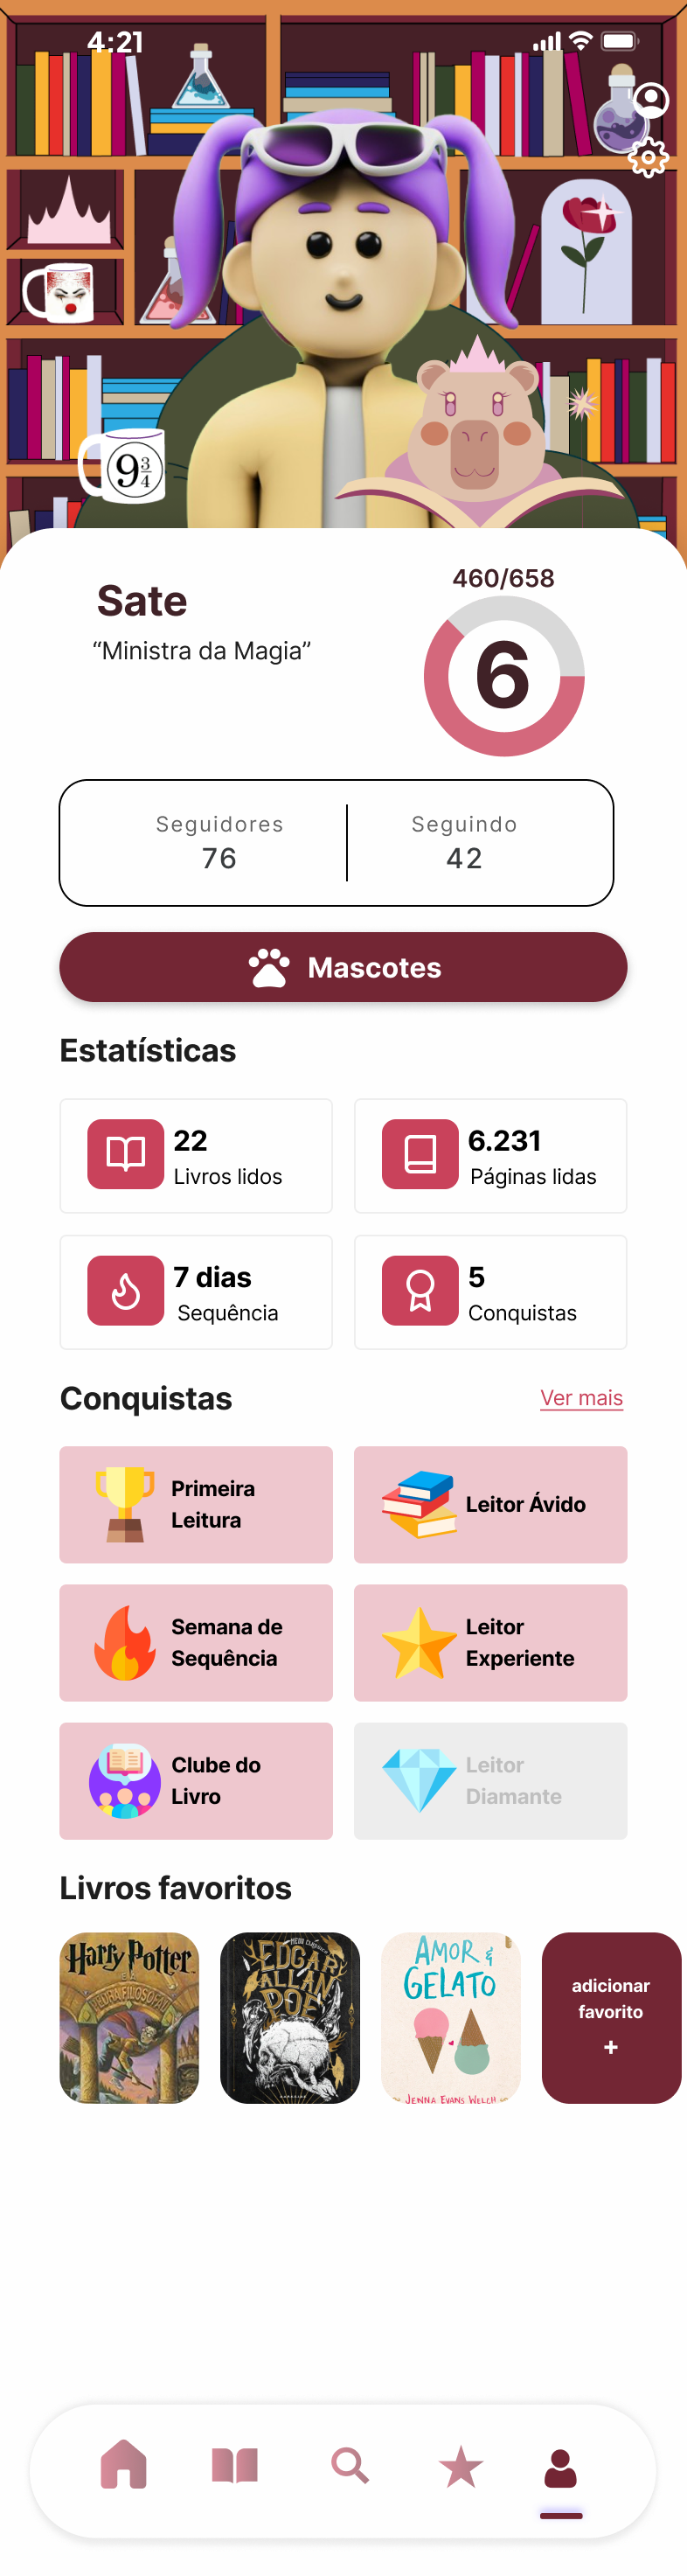
\includegraphics[width=0.43\linewidth,height=0.45\textheight,keepaspectratio]{conteudo/5 - ages IV/conteudo/figures/perfil.png}
\caption{Protótipos do detalhe do livro e do perfil do usuário.}
\legend{Fonte: exportações do Figma mantidas no repositório AGESIV.}
\end{figure}

\subsection{Tecnologias Utilizadas}

O mobile utiliza React Native, Expo, TypeScript, expo-router e NativeWind. O backend utiliza Java 21, Spring Boot, Spring Data JPA, Maven e Springdoc OpenAPI para documentação dos endpoints. A persistência utiliza PostgreSQL e Flyway. Docker e Docker Compose apoiam a execução local, e GitHub Actions executa verificações automatizadas.

O backend conta com testes unitários e de integração, incluindo Testcontainers, além de JaCoCo para cobertura e Spotless para formatação. No mobile, há verificações de tipos e testes de componentes. As configurações e convenções estão documentadas no README do repositório de código.

\clearpage
\section{Atividades Desempenhadas Pelo Aluno no Projeto}
\subsection{Sprint 0}

Na preparação do ReadRace, participei das discussões iniciais com os demais AGES IV para compreender a proposta e organizar a condução do projeto. Nessas reuniões, definimos perguntas aos stakeholders e planejamos as atividades em aula. Também contribuí com a prototipação de telas e a escrita das user stories. Esse trabalho exigiu transformar a proposta ampla de incentivo à leitura em fluxos e decisões que pudessem orientar o desenvolvimento.

O planejamento documentado foi organizado em fundação do projeto, componentes compartilhados, biblioteca, detalhe e progresso de leitura, interação social, desafios e busca. Várias entregas dependiam de elementos comuns, como tema, componentes, schema e dados iniciais. O diagrama de dependências compartilhado entre os AGES IV ajudou a discutir a ordem de execução e os impactos de tarefas que permanecessem paradas.

Mantive contato com os colegas de gestão e fiz uma leitura inicial da documentação relacionada às capas dos livros. Na revisão da modelagem do banco, verifiquei discrepâncias entre as user stories da Sprint 1 e o modelo relacional, fiz anotações e conversei com os colegas para encaminhar os pontos aos AGES III. Discutimos as dúvidas e elaboramos sugestões de melhoria. Essa experiência mostrou que requisitos e dados precisam evoluir de forma coordenada: uma regra pouco clara pode gerar interpretações distintas na API e na interface.

Outro eixo da minha participação foi a preparação das apresentações. Trabalhei na criação dos slides para apresentar aos clientes os fluxos e as histórias priorizadas para a Sprint 1. A versão inicial ainda exigia ajustes, e sua construção me ajudou a organizar o que seria comunicado e a distinguir a visão completa do produto do recorte daquela entrega.

O cronograma previa a apresentação das user stories e dos mockups aos stakeholders e o planejamento da Sprint 1 em 24 de agosto de 2026, às 17h30. A retrospectiva da Sprint 0 e a entrega do relatório no Fluxo AGES estavam previstas para 26 de agosto, no mesmo horário. Esses marcos ajudam a situar a preparação do escopo e das primeiras entregas.

Essa preparação também teve importância pessoal. Apresentar para os stakeholders foi um grande desafio para mim por conta da timidez. Participei ativamente das apresentações ao lado dos demais colegas de AGES IV, exercitando a exposição de ideias e a comunicação com pessoas externas à equipe. Esse contato foi uma oportunidade de desenvolvimento além da implementação de software.

\subsection{Sprint 1}

A Sprint 1 concentrou o desenvolvimento de uma versão navegável do ReadRace para apresentação aos clientes. Planejamos a base mobile e backend, os componentes reutilizáveis e as funcionalidades de biblioteca, registro de progresso, interação social, busca, perfil de outro usuário e desafios entre amigos.

Minha atuação combinou desenvolvimento, revisão e gestão. Revisei o PR de migration e seed, participei dos alinhamentos da equipe e concluí atividades relacionadas aos componentes BookCover e EmptyState. Também revisei a tarefa de busca de usuários, livros e comunidades e avancei no desenvolvimento do perfil de usuários.

Participei da resolução de conflitos e da integração de entregas de colegas. Revisei PRs ligados à API de desafios e à biblioteca, levantando a necessidade de avaliar paginação nas listagens. Também trabalhei no componente BottomSheet, no cálculo de XP associado ao registro de leitura, no componente Card, na tela de detalhe do livro e no componente ListItem. Na reta final, desenvolvi e ajustei a API e a tela de visualização do perfil de outro usuário.

A implementação do registro de leitura exigiu atenção à diferença entre a página atual e a página máxima já alcançada. A regra de XP precisava impedir que a mesma página fosse contabilizada novamente ao retroceder e avançar na leitura.

Durante as aulas, procurei acompanhar o que os colegas estavam fazendo, perguntar sobre o andamento das tarefas e oferecer ajuda. Fora da sala, também entrei em contato para verificar entregas, apoiar a entrada de colegas no GitHub e lembrar a equipe das revisões pendentes. Reforcei os avisos sobre o code freeze e a necessidade de concluir tarefas das quais outras entregas dependiam.

Apesar dessas iniciativas, reconheço que nós, AGES IV, deveríamos ter acompanhado o projeto de maneira mais contínua. Faltou cobrar atualizações com antecedência e manter uma visão mais próxima das dificuldades de cada integrante. Na aproximação da entrega, precisei assumir várias tarefas para reduzir as pendências. Minha disponibilidade para ajudar foi positiva, mas a concentração de implementação no final também evidenciou uma falha no acompanhamento e na distribuição do trabalho.

Na preparação da entrega, discutimos o estado do projeto e um plano para as tarefas críticas, buscando contato com seus responsáveis e avaliando a necessidade de assumir entregas sem perspectiva de conclusão no prazo. Trabalhei em ajustes e conflitos relacionados ao detalhamento do livro e reforcei a comunicação sobre a weekly e o encerramento do desenvolvimento. Também participei do alinhamento das prioridades da apresentação, dos ajustes do perfil público e da organização das atividades da equipe.

Na apresentação aos stakeholders, demonstramos a biblioteca, o detalhe do livro e o registro de progresso, o feed de comunidades, a página do clube com ranking, o fórum, a busca e o perfil de outro leitor. O material de entrega, datado de 18 de setembro de 2026, registra 32 tarefas entregues, oito telas, 17 endpoints e 16 componentes como resultado coletivo. As telas do fluxo de desafios entre amigos ainda foram apresentadas como design, com implementação prevista para a Sprint 2. A demonstração da interface social se concentrou na consulta às informações de comunidades, clubes e leitores.

Na retrospectiva, expliquei que os bloqueios precisam ser comunicados e tratados rapidamente. Uma tarefa parada pode impedir outras entregas e comprometer o projeto inteiro, especialmente nos fluxos com dependências encadeadas. A principal lição foi que a gestão precisa identificar esses sinais durante a sprint, e não apenas quando o prazo está próximo.

Como resultado da retrospectiva, definimos a divisão do time em squads com um ou dois integrantes de AGES IV em cada grupo. Essa decisão buscou aproximar os responsáveis dos desenvolvedores e facilitar a identificação de impedimentos e o acompanhamento das entregas.

Também participei da apresentação aos stakeholders ao lado dos colegas de gestão, explicando as funcionalidades demonstradas e o trabalho realizado pela equipe. No cronograma, a apresentação da Sprint 1 e o planejamento da Sprint 2 estavam previstos para 14 de setembro de 2026, às 17h30. Para 16 de setembro, no mesmo horário, estavam previstas a retrospectiva, a entrega do relatório da sprint no Fluxo AGES e a entrega do Relatório de Acompanhamento no formato de memorial descritivo. Esses marcos de programação são distintos da data de 18 de setembro registrada no material de entrega.

\clearpage
\subsection{Sprint 2}

A \textit{Sprint} 2 teve como objetivo dar continuidade à primeira versão navegável do ReadRace e conectar funcionalidades que ainda estavam parcialmente isoladas. Uma das prioridades foi concluir o fluxo de desafios entre amigos, pendente da \textit{Sprint} 1. Também estava prevista a integração do registro de leitura ao \ac{XP} acumulado, ao nível do usuário, à sequência de dias, ao progresso dos desafios e às conquistas. Essa integração era importante para que registrar uma leitura produzisse efeitos perceptíveis no restante da experiência do aplicativo.

O planejamento incluía as telas de Perfil e Minhas Conquistas, a possibilidade de curtir e descurtir posts e a correção de pendências de navegação, apresentação visual, acessibilidade e testes automatizados. Inicialmente, também seriam trabalhadas a participação em comunidades, a página da comunidade e a adição de livros. Entretanto, a redução da duração da \textit{sprint} de quatro para duas semanas exigiu rever os compromissos. A apresentação de entrega da \textit{Sprint} 2 registra essa revisão de 21 tarefas inicialmente apresentadas para 18 no plano final. As três tarefas retiradas foram transferidas para a \textit{Sprint} 3, delimitando o que seria efetivamente entregue naquele intervalo.

Além dessa revisão das tarefas da \textit{sprint}, conversamos com os clientes sobre a retirada dos eventos globais do escopo do produto. A proposta já estava muito ampla, e esse alinhamento permitiu concentrar o trabalho no que seria viável entregar. Essa negociação foi importante para que a redução de escopo fosse uma decisão compartilhada e para manter uma expectativa clara sobre o resultado do semestre.

Na organização da equipe, passei a acompanhar a frente de Social, biblioteca e qualidade, junto ao colega Guilherme Bohm, também \ac{AGES} IV. Criei um grupo de WhatsApp para facilitar a comunicação e compartilhei as tarefas e seus links: curtir e descurtir posts (\href{https://github.com/ReadRace-AGES/ReadRace/issues/101}{issue \#101}), corrigir o retorno do detalhe do livro para a Busca (\href{https://github.com/ReadRace-AGES/ReadRace/issues/102}{\#102}), remover rotas de teste fora do produto (\href{https://github.com/ReadRace-AGES/ReadRace/issues/103}{\#103}) e substituir o aviso local da biblioteca pelo Toast compartilhado (\href{https://github.com/ReadRace-AGES/ReadRace/issues/104}{\#104}). Deixei os colegas escolherem as tarefas e me coloquei, junto ao Guilherme, à disposição para esclarecer dúvidas de requisitos e de desenvolvimento.

O acompanhamento ocorreu pelo WhatsApp e diretamente nas aulas; com os \ac{AGES} III do \textit{squad}, utilizei mais o Discord. A divisão funcionou muito bem para manter um trabalho mais consistente e direto com os colegas. Conseguimos reduzir a necessidade de os \ac{AGES} IV assumirem implementações para compensar dificuldades da equipe, preservando espaço para que os demais integrantes conduzissem suas entregas. Os registros do repositório mostram essa distribuição: as curtidas foram implementadas no \href{https://github.com/ReadRace-AGES/ReadRace/pull/112}{PR \#112}, de \texttt{arthurgreco}; a retirada de rotas, no \href{https://github.com/ReadRace-AGES/ReadRace/pull/114}{PR \#114}, de \texttt{gugs123}; e a troca do aviso pelo Toast, no \href{https://github.com/ReadRace-AGES/ReadRace/pull/123}{PR \#123}, de \texttt{oEduardoCastro}.

Minha contribuição direta de implementação nessa \textit{sprint} foi a correção de navegação da issue \#102, integrada pelo \href{https://github.com/ReadRace-AGES/ReadRace/pull/124}{PR \#124}. Ao abrir um livro pela Busca, o retorno podia levar à aba errada porque Busca e Meus Livros compartilhavam o mesmo caminho de rota. Separei os caminhos por aba, mantendo a tela de detalhe compartilhada, de forma a preservar o termo e os resultados da pesquisa e a pilha de navegação de origem. Também foram adicionados testes de retorno nos estados de carregamento, erro e sucesso e após o registro de progresso. Essa tarefa mostrou como um problema de navegação aparentemente pequeno podia comprometer a continuidade da experiência de uso.

Ao final, a equipe concluiu as 18 tarefas do escopo revisado, incluindo seis novas telas. Nos desafios entre amigos, foram entregues a criação de desafios por páginas ou por livro, a escolha da obra, o acompanhamento do placar e a apresentação dos resultados de vitória, derrota ou empate. Esses fluxos foram construídos em contribuições de diferentes colegas, como os \href{https://github.com/ReadRace-AGES/ReadRace/pull/115}{PRs \#115}, \href{https://github.com/ReadRace-AGES/ReadRace/pull/121}{\#121}, \href{https://github.com/ReadRace-AGES/ReadRace/pull/122}{\#122} e \href{https://github.com/ReadRace-AGES/ReadRace/pull/126}{\#126}. Minha atuação de gestão apoiava esse esforço coletivo por meio da comunicação e do acompanhamento das tarefas.

Também foram entregues Perfil, Minhas Conquistas e as interações de curtida e descurtida. Houve correções na navegação e na exibição de capas, ajustes de layout no celular e a inclusão de testes do \textit{mobile} na integração contínua. Como entrega adicional da equipe, foi estruturada a infraestrutura \ac{AWS} com configuração de \textit{deploy} automático. A integração da leitura ao total de \ac{XP} e ao nível foi registrada no \href{https://github.com/ReadRace-AGES/ReadRace/pull/127}{PR \#127}; a sequência de dias, no \href{https://github.com/ReadRace-AGES/ReadRace/pull/125}{PR \#125}; e conquistas e seu desbloqueio automático, no \href{https://github.com/ReadRace-AGES/ReadRace/pull/118}{PR \#118}. Essas mudanças conectaram o registro de leitura à progressão do usuário.

Essa etapa deu continuidade ao trabalho com registro de leitura e cálculo de \ac{XP} no qual eu havia atuado na \textit{Sprint} 1. Para mim, a evolução do produto tornou mais evidente que uma regra aparentemente localizada pode afetar diversas partes da aplicação. O progresso de leitura precisava manter coerência com nível, desafios e conquistas, o que aumentava a importância de alinhar o comportamento esperado entre as diferentes frentes de desenvolvimento.

O cronograma situou a apresentação da \textit{Sprint} 2 aos \textit{stakeholders} e o planejamento da \textit{Sprint} 3 em 2 de outubro de 2026, às 19h15. Para a mesma data, às 21h, estavam previstas a retrospectiva e a entrega do relatório de andamento no Fluxo \ac{AGES}. Conduzi a apresentação dessa \textit{sprint}, assumindo de forma mais direta um desafio que havia estabelecido para a \ac{AGES} IV: melhorar minhas habilidades de comunicação e apresentação. Preparar o conteúdo e explicar as entregas aos clientes passou a ser uma parte importante da minha atuação de gestão.

A principal lição de processo foi a necessidade de ajustar o escopo à duração real da \textit{sprint} e explicitar as transferências de tarefas. A conclusão do escopo revisado precisava ser compreendida junto dessa mudança, mantendo visibilidade sobre o que continuava pendente. Para a etapa seguinte, permaneceram demandas de autenticação e disponibilização do aplicativo instalável, além da expansão dos clubes, comunidades, biblioteca e recursos de personalização. Assim, a \textit{Sprint} 2 ampliou a integração do produto, mas ainda não representou o encerramento das funcionalidades planejadas para o semestre.

\subsection{Sprint 3}
A Sprint 3 ampliou os recursos sociais do ReadRace e trouxe o desafio de aproximar a aplicação de uma experiência utilizável fora do ambiente de desenvolvimento. O planejamento contemplava criação de clubes, chat, publicação no fórum, saída do clube e ranking completo. Também incluía configuração e resposta a quizzes, pontuação por acertos e leitura, acompanhamento de comunidades e leitores, adição de livros pelo catálogo, autenticação, personalização e disponibilização de um aplicativo instalável para Android.

No resultado coletivo, foram concluídas 16 das 17 tarefas do planejamento apresentado, além das duas tarefas de reserva: comentários em comunidades e seguir leitores. A equipe entregou fluxos de clubes, quiz e pontuação, biblioteca, login, cadastro, acesso com Google, personalização e revanche entre amigos, além de logs e alarmes de produção. Foram antecipados o acompanhamento dos desafios semanais e mensais, as listas de seguidores e seguidos e um ajuste do ranking para demonstração, inicialmente previstos para a Sprint 4. Também foram adicionados avatar e plano de fundo ao perfil. O pagamento de XP dos desafios semanais e mensais, entretanto, permaneceu para a próxima sprint.

Minha contribuição individual esteve relacionada principalmente às funcionalidades de acompanhamento de leitores, à visualização de seguidores e seguidos e ao apoio à integração das entregas do squad. Os registros pessoais de atividades fora de aula ajudam a identificar essa participação. Em 9 de outubro de 2026, registrei trabalho de desenvolvimento na issue de seguir outros usuários, associado a atividades de desenvolvimento e testes. Essa funcionalidade ampliava a relação entre os leitores para além da consulta a um perfil, oferecendo uma base para acompanhar outras pessoas dentro da plataforma.

Em 19 de outubro, trabalhei na comunicação com os colegas do squad, na resolução de conflitos de código e na revisão da issue de adição de um novo livro à biblioteca. Também realizei revisão e resolução de problemas na funcionalidade de abertura do perfil de uma comunidade e nas ações de seguir ou deixar de seguir. Essas atividades exigiram acompanhar entregas de colegas e observar como elas se conectavam aos fluxos que já existiam no aplicativo. Minha atuação, portanto, combinou implementação com revisão e apoio à organização do trabalho.

Ainda em 19 de outubro, em outro período registrado, dediquei-me ao desenvolvimento da issue de visualização de seguidos e seguidores. Essa entrega complementava a possibilidade de seguir leitores, tornando essas relações consultáveis na interface. O trabalho reforçou uma percepção que já vinha aparecendo nas sprints anteriores: funcionalidades relacionadas precisam ser tratadas como partes de uma experiência contínua, pois concluir uma ação sem oferecer uma forma clara de consultar seu resultado limita a utilidade para o usuário.

Um dos desafios coletivos da sprint foi integrar funcionalidades que alteravam as mesmas telas. A necessidade de resolver conflitos e revisar entregas relacionadas mostrou a importância de alinhar previamente os pontos de contato entre tarefas. Para mim, o aprendizado esteve na combinação entre atenção ao código e comunicação com o squad: a revisão precisava considerar também o fluxo de uso e os impactos das mudanças sobre o trabalho dos demais colegas.

Na validação do produto, foi identificado um problema nas capas dos livros no aplicativo instalado, corrigido com o uso de HTTPS. Esse episódio mostrou que o funcionamento no ambiente de desenvolvimento não garantia o mesmo comportamento em um Android real. A disponibilização completa do instalável não foi encerrada na sprint: ainda era necessário finalizar a distribuição e validar a autenticação em produção. A documentação do banco de dados também permaneceu pendente.

Essas pendências reforçaram a necessidade de distinguir implementação, publicação em produção e disponibilização ao usuário nos critérios de conclusão. Para a Sprint 4, ficaram previstos o fechamento da distribuição Android com login, o pagamento de XP dos desafios semanais e mensais, a apresentação imediata das recompensas de leitura e a aba Social com atividades dos leitores seguidos. Também permaneceram ajustes nos fluxos de clubes, biblioteca e publicações, a finalização da documentação e os testes no aplicativo instalado. Naquele planejamento, a entrega final estava prevista para 18 de novembro de 2026; os resultados dessa etapa ainda não são apresentados neste relato.

\subsection{Sprint 4}

A Sprint 4 foi a última etapa do ReadRace, encerrada com a entrega de 13 de novembro de 2026. Sua preparação combinou funcionalidades ainda previstas com a necessidade de revisar o comportamento da aplicação integrada. O planejamento herdado da sprint anterior incluía a distribuição do aplicativo Android com login, os ajustes nas recompensas de leitura e nos desafios semanais e mensais, além da evolução dos fluxos sociais, da biblioteca e da documentação. Minha participação envolveu testes, correções, revisão de código, melhorias de interface e preparação e condução da apresentação final.

Em 30 de outubro, dediquei-me a mapear bugs na versão implantada da aplicação. O trabalho envolveu testar o sistema, documentar os erros encontrados e preparar o desenvolvimento das correções. Essa atividade mudou o foco da minha participação: além de acompanhar funcionalidades isoladas, passei a observar o comportamento do produto integrado. A avaliação de uso foi realizada por nós, os próprios desenvolvedores. Foi ao utilizar o aplicativo que percebi problemas de UX e que a biblioteca tinha uma apresentação pouco atraente e pouco amigável. Essa percepção orientou minha revisão da interface, procurando tornar as informações mais organizadas e as ações de leitura mais fáceis de encontrar.

Em 3 de novembro, dei continuidade a esse trabalho desenvolvendo e testando correções para os bugs encontrados durante a utilização da aplicação. Um exemplo concreto foi integrado pelo \href{https://github.com/ReadRace-AGES/ReadRace/pull/259}{PR \#259}, de minha autoria: corrigi os cards de grupos que perdiam alinhamento no Android e a biblioteca que permanecia desatualizada após registrar leitura ou adicionar livros. A atualização passou a ocorrer ao retornar à tela, preservando os itens já explorados e o conteúdo exibido durante a consulta. Essa tarefa mostrou que uma funcionalidade podia gravar os dados corretamente e, ainda assim, transmitir uma impressão errada ao usuário se a interface não refletisse a alteração.

Em 11 de novembro, atuei na revisão de pull requests e na integração da aplicação com Playwright. Esse trabalho foi integrado pelo \href{https://github.com/ReadRace-AGES/ReadRace/pull/265}{PR \#265}, de minha autoria, relacionado à \href{https://github.com/ReadRace-AGES/ReadRace/issues/233}{issue \#233}. Configurei testes de ponta a ponta para a versão web do aplicativo em dimensões de celular, com API e PostgreSQL reais em ambiente isolado. O PR registra 22 testes aprovados localmente, sem repetição automática, cobrindo fluxos de biblioteca, leitura, busca, comunidades, clubes, desafios e perfil. O roteiro autenticado com Cognito e a execução no CI ainda exigiam validação naquele registro; os testes de navegador também não substituíam a verificação no Android.

Outra contribuição importante foi o \href{https://github.com/ReadRace-AGES/ReadRace/pull/266}{PR \#266}, no qual trabalhei na experiência de uso e na apresentação visual da biblioteca. Dei mais destaque à leitura em andamento, com título, autor, progresso e acesso direto ao registro de páginas, organizei os filtros das listas e tornei a ação de adicionar livro mais visível. Também melhorei os estados vazios e a identificação das obras quando as capas não carregavam. A revisão se estendeu à clareza da busca, à hierarquia de ações do clube e aos rótulos da navegação. Essas mudanças ajudaram a tornar mais compreensíveis funcionalidades que já existiam.

A Figura~\ref{fig:readrace-biblioteca-ux} apresenta a comparação utilizada na entrega final. Na versão anterior, o cabeçalho e as seções de capas ocupavam grande parte da área inicial. Na versão revisada, o livro em andamento passou a reunir identificação, progresso e registro de leitura em destaque. A comparação ilustra mudanças de hierarquia e de acesso às ações; as capturas usam dados e momentos diferentes e não constituem um teste de usabilidade com leitores.

\begin{figure}[H]
    \centering
    \caption{Biblioteca do ReadRace antes e depois da revisão de UX/UI}
    \label{fig:readrace-biblioteca-ux}
    \begin{minipage}{0.45\linewidth}
        \centering
        {\small Antes da revisão}\par\smallskip
        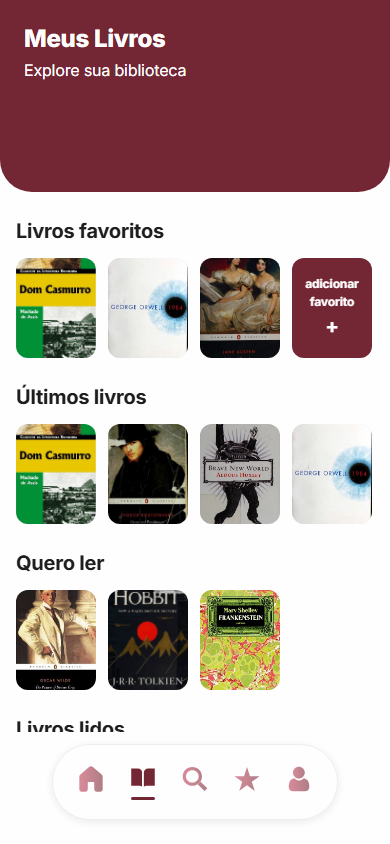
\includegraphics[width=\linewidth,height=0.48\textheight,keepaspectratio]{conteudo/5 - ages IV/conteudo/figures/biblioteca-antes-ui.png}
    \end{minipage}
    \hfill
    \begin{minipage}{0.45\linewidth}
        \centering
        {\small Depois da revisão}\par\smallskip
        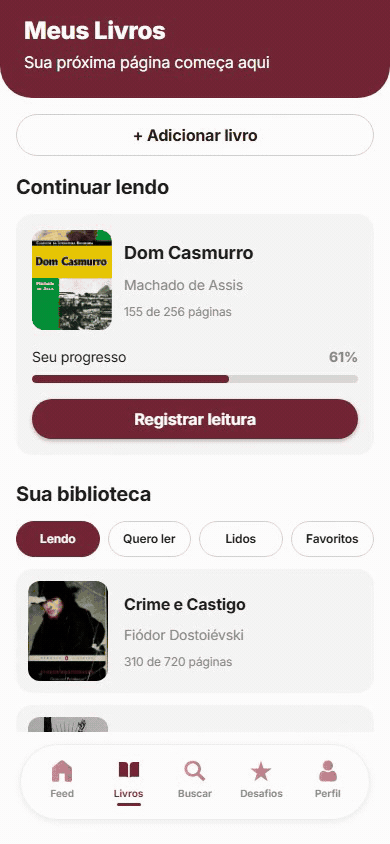
\includegraphics[width=\linewidth,height=0.48\textheight,keepaspectratio]{conteudo/5 - ages IV/conteudo/figures/biblioteca-depois-ui.png}
    \end{minipage}
    \legend{Fonte: apresentação ReadRace --- Sprint 4, Entrega Final, slide 13. Antes: inspeção de 11/11/2026. Depois: quadro extraído da demonstração em GIF.}
\end{figure}

A apresentação final registra 30 testes locais: nove verificações dos fluxos principais, 13 regressões e oito verificações de UX. O material descreve execução com Chromium, API real e PostgreSQL temporário, restaurando os dados entre os testes. Esses números se referem à preparação local da apresentação e complementam os 22 testes descritos inicialmente no PR \#265. As verificações de UX contemplaram telas pequenas, estados vazios e registro direto de leitura. A revisão de interface apresentada foi heurística, sem métricas de avaliação com leitores.

No dia 12 de novembro, trabalhei em correções finais de preparação para a entrega e no desenvolvimento dos slides da apresentação. Na reta final, também implementei a criação de comunidades pelo Feed, integrada pelo \href{https://github.com/ReadRace-AGES/ReadRace/pull/268}{PR \#268}. A funcionalidade inclui formulário, validação, criação conjunta da comunidade e de seu administrador e atualização da lista de comunidades do usuário. A capa é opcional por URL HTTPS; upload de arquivos, edição e transferência de administração ficaram para uma evolução posterior. Também abri o \href{https://github.com/ReadRace-AGES/ReadRace/pull/273}{PR \#273}, que integrou a branch de desenvolvimento à principal no dia da entrega.

No resultado coletivo, algumas pendências das sprints anteriores tiveram seu fechamento registrado no repositório. O \href{https://github.com/ReadRace-AGES/ReadRace/pull/232}{PR \#232} integrou o pagamento de XP dos desafios semanais e mensais; o \href{https://github.com/ReadRace-AGES/ReadRace/pull/254}{PR \#254} passou a apresentar as recompensas logo após o registro de leitura; e o \href{https://github.com/ReadRace-AGES/ReadRace/pull/261}{PR \#261} corrigiu situações que permitiam obter recompensas sem avanço real. A distribuição Android foi tratada no \href{https://github.com/ReadRace-AGES/ReadRace/pull/243}{PR \#243}, que documenta a geração e validação do APK com login contra a API de produção. A disponibilização ocorreu por link de distribuição interna, com Android como plataforma da entrega, sem publicação em loja.

Na demonstração final, organizamos o produto como uma jornada entre Feed, Meus Livros, Busca, Desafios e Perfil. O material apresentou o registro direto de páginas na biblioteca e seu retorno de recompensas, as atividades de leitura das pessoas seguidas, a descoberta e os pedidos de entrada em clubes e a participação em comunidades. Também explicitou os limites do escopo consolidado: iOS, publicação na Play Store, notificações, canal de suporte, enquetes, eventos, recomendações de livros, ranking global e painel administrativo ficaram fora da entrega. Registrar esses cortes ajudava a comunicar com clareza as fronteiras do produto que estava sendo apresentado.

Essas atividades reforçaram minha percepção de que a qualidade de uma entrega depende de um acompanhamento que continua depois da implementação inicial. O mapeamento de bugs, as correções, os testes, a revisão de código e a preparação da apresentação compunham um mesmo esforço de tornar o produto mais consistente e de comunicar seu estado com clareza. Também ficou mais evidente a necessidade de conciliar o tempo dedicado a resolver problemas com a organização das tarefas de encerramento.

Conduzi a apresentação final, assim como havia feito nas Sprints 2 e 3. Esse foi um dos desafios pessoais que estabeleci para a AGES IV: desenvolver minhas soft skills, especialmente a comunicação em apresentações. Preparar os slides, conhecer o estado do produto e explicar o trabalho aos stakeholders me permitiu exercitar essa habilidade de forma recorrente. A evolução da minha participação foi de auxiliar nas primeiras apresentações para assumir a condução das entregas seguintes.

Encerramos o projeto em 13 de novembro com a entrega do que havia sido combinado com os clientes, considerando os ajustes de escopo negociados ao longo do semestre. Eles demonstraram muita satisfação com o resultado e destacaram a diferença percebida entre as Sprints 3 e 4, especialmente as refatorações de UX/UI na biblioteca. Esse retorno foi importante porque mostrou o valor de dedicar esforço à clareza e à organização da experiência de uso, além de ampliar a quantidade de funcionalidades. Também concluímos a documentação de encerramento, incluindo o inventário final do Figma, o registro das diferenças na wiki e os materiais de operação. Esses materiais fizeram parte do fechamento do projeto e da entrega à disposição dos clientes.


\section{Conclusão}

Na \ac{AGES} IV, a principal mudança na minha atuação foi assumir mais responsabilidades de gestão. No ReadRace, precisei conciliar o desenvolvimento e a revisão de código com o acompanhamento das tarefas e a comunicação com os colegas e os \textit{stakeholders}.

No trabalho técnico, a revisão da modelagem e a implementação do progresso de leitura me fizeram retomar as histórias de usuário para entender como as regras deveriam funcionar na aplicação. Essas atividades aproximaram os conhecimentos de requisitos, banco de dados e desenvolvimento trabalhados ao longo do curso.

Nas primeiras \textit{sprints}, minha principal autocrítica foi o acompanhamento da equipe. Assumir implementações perto do prazo ajudou na entrega, mas mostrou que eu precisava perceber as dificuldades dos colegas mais cedo. A divisão em \textit{squads} respondeu bem a esse problema: o acompanhamento pelo WhatsApp, pelo Discord e nas aulas tornou o trabalho mais direto e reduziu a necessidade de os \ac{AGES} IV assumirem tarefas de implementação para compensar atrasos. Essa experiência reforçou a importância de oferecer apoio e manter os responsáveis próximos, preservando a autonomia dos colegas.

As apresentações aos \textit{stakeholders} também contribuíram para meu desenvolvimento. A timidez era uma dificuldade que eu desejava trabalhar nessa \ac{AGES}, e conduzi as apresentações das \textit{Sprints} 2, 3 e 4. Preparar os slides e assumir a exposição das entregas permitiu praticar a comunicação com os clientes em diferentes momentos. Considero esse avanço uma parte importante da minha experiência, pois exigiu transformar conhecimento técnico e acompanhamento do projeto em uma explicação clara do produto.

Nas \textit{Sprints} 2 e 3, a evolução dos recursos de progressão e interação social reforçou a importância de integrar as funcionalidades ao fluxo completo do produto. Minha participação no acompanhamento de leitores, nas listas de seguidores e seguidos e nas revisões das entregas do \textit{squad} também ampliou minha experiência com funcionalidades que dependem do trabalho de diferentes integrantes.

Na preparação da entrega da \textit{Sprint} 4, passei a dedicar mais atenção ao mapeamento de bugs na versão implantada, ao desenvolvimento e teste de correções e à revisão das integrações. O trabalho com Playwright e a preparação dos slides também ampliaram minha participação nas atividades de qualidade e comunicação. Essa etapa reforçou que acompanhar uma entrega envolve observar o produto em funcionamento e organizar sua apresentação, além de concluir implementações.

O projeto foi encerrado com a entrega da \textit{Sprint} 4 em 13 de novembro de 2026, atendendo ao escopo combinado após os alinhamentos com os clientes. O retorno positivo destacou a evolução entre as \textit{Sprints} 3 e 4 e as melhorias de \ac{UX}/\ac{UI} na biblioteca, uma frente em que atuei diretamente. A autenticação foi implementada por outros colegas e minha participação incluiu os testes iniciais de acesso; o repositório também documenta a disponibilização do \ac{APK} Android com \textit{login} e \ac{API} de produção. Essas distinções ajudam a reconhecer tanto minha contribuição quanto o resultado construído pela equipe.

Entre os quatro projetos da minha trajetória na \ac{AGES}, considero o ReadRace o melhor para mim. O principal motivo foi a evolução em gestão e desenvolvimento pessoal: acompanhar colegas, organizar entregas e conduzir apresentações me permitiu trabalhar habilidades que eu havia estabelecido como desafios desta etapa. Essa avaliação considera meu processo de formação, além das funcionalidades entregues.

A revisão do escopo e o acompanhamento dos \textit{squads} aproximaram essa experiência de Processos de Software e Gerenciamento de Projetos de Software. O trabalho com modelagem, integrações e testes também retomou conhecimentos de banco de dados, arquitetura e verificação e validação. A articulação entre essas áreas ficou mais evidente quando passei a acompanhar a entrega do produto integrado.



\chapter[Considerações finais]{CONSIDERAÇÕES FINAIS}

\section{Relação entre as disciplinas e a prática}

Considero que todas as disciplinas do curso contribuíram para minha atuação na \ac{AGES}, ainda que essa relação nem sempre fosse imediata. Mesmo os conteúdos mais teóricos, matemáticos e ligados aos fundamentos da computação ajudaram a construir meu raciocínio lógico. Ao longo dos projetos, passei a perceber melhor o valor dessa base para decompor problemas, compreender relações entre informações e analisar alternativas antes de implementar uma solução. Por isso, não associo a contribuição de uma disciplina apenas ao uso direto de uma tecnologia estudada em aula.

Entre as contribuições que reconheço com mais clareza estão as disciplinas ligadas à gestão e ao desenvolvimento ágil. Na matriz do curso, essa formação aparece em componentes como Processos de Software e Gerenciamento de Projetos de Software. O planejamento das \textit{sprints}, a organização das tarefas, as revisões de escopo e o acompanhamento dos \textit{squads} foram oportunidades de aproximar esses conhecimentos da prática. No ReadRace, por exemplo, a redução do tempo disponível para a \textit{Sprint} 2 exigiu rever os compromissos assumidos, enquanto a divisão em \textit{squads} tornou o acompanhamento dos colegas mais direto. Essas situações me ajudaram a compreender a importância de adaptar o planejamento às condições reais da equipe.

Também destaco Projeto e Arquitetura de Software, pela contribuição para compreender a organização das aplicações e as relações entre suas partes. Essa perspectiva se relaciona ao trabalho que realizei com \textit{backend}, modelagem de dados e revisão de integrações. Em diferentes projetos, precisei considerar como uma alteração afetaria outras funcionalidades, além de entender o trecho de código em que estava trabalhando. A experiência com banco de dados, desde a \ac{AGES} II, também aproximou minha prática dos conhecimentos de Banco de Dados I e II, especialmente na organização das entidades e de seus relacionamentos.

As quatro passagens pela \ac{AGES} permitiram reunir conhecimentos que, nas disciplinas, eram apresentados com focos distintos. Na execução de um projeto, requisitos, arquitetura, implementação, qualidade e gestão se relacionam continuamente. Essa vivência ampliou minha percepção sobre a formação em Engenharia de Software e sobre a importância de manter uma base ampla para lidar com problemas que não se limitam a uma única área do curso.

\section{Aprendizados ao longo das quatro AGES}

Quando iniciei minha trajetória na \ac{AGES}, ainda não tinha experiência com o desenvolvimento de software em projetos reais. Ao longo das quatro passagens, pude construir uma compreensão mais ampla desse trabalho, vivenciando diferentes processos e os desafios técnicos envolvidos em sua execução. O contato com levantamento de requisitos, planejamento, modelagem, implementação, testes, correções e entrega me permitiu acompanhar etapas do ciclo de vida de um software e entender como elas dependem umas das outras.

Um dos aprendizados mais importantes foi reconhecer o valor de planejar antes de executar. Compreender a necessidade do cliente, discutir as alternativas e organizar as tarefas passou a fazer mais sentido à medida que eu percebia o impacto dessas decisões no desenvolvimento. As experiências com dúvidas de requisitos, dependências entre funcionalidades e ajustes de escopo mostraram que a preparação faz parte da construção da solução e influencia o resultado do trabalho técnico.

Também aprendi, pela convivência com as equipes, quanto a comunicação interfere no sucesso de um projeto. Explicar uma tarefa com clareza, ouvir as dificuldades de um colega e alinhar expectativas são ações que ajudam cada integrante a contribuir melhor. Conforme assumi mais responsabilidades, percebi que acompanhar o trabalho exigia entender o que as pessoas precisavam para avançar e encontrar uma forma adequada de orientá-las. A experiência de desenvolver junto de colegas com diferentes conhecimentos tornou esse aprendizado especialmente significativo.

Essa trajetória ampliou minha visão da Engenharia de Software. Passei a compreender o desenvolvimento como um trabalho que reúne conhecimento técnico, planejamento e colaboração durante a evolução do produto. Hoje, reconheço a importância de dedicar atenção tanto à solução implementada quanto às condições em que a equipe a constrói, pois a qualidade da comunicação e da organização influencia diretamente o que conseguimos entregar juntos.

\section{Direção profissional}

Desde que ingressei em Engenharia de Software, meu interesse estava voltado a uma carreira mais técnica. A arquitetura de software era o caminho que eu desejava seguir, por isso as oportunidades de aprofundar meus conhecimentos de \textit{backend}, modelagem e organização das aplicações tinham especial importância para mim.

As experiências nas \ac{AGES} III e IV ampliaram essa perspectiva. O contato mais próximo com a organização das equipes e o acompanhamento das entregas me permitiu conhecer responsabilidades que passaram a fazer parte das minhas possibilidades de carreira. Ao mesmo tempo, a presença crescente da inteligência artificial no desenvolvimento de software me levou a refletir sobre o direcionamento que gostaria de dar à minha atuação. Considerando essas experiências e minha leitura desse contexto, vejo a gestão como a melhor alternativa profissional para mim neste momento.

Essa percepção ajuda a explicar a atenção que tenho dedicado ao desenvolvimento das minhas \textit{soft skills}. Conduzir as apresentações das \textit{Sprints} 2, 3 e 4 e acompanhar os colegas foram oportunidades de praticar habilidades que considero importantes para essa direção. Quero continuar aprimorando minha comunicação e minha capacidade de orientar o trabalho em equipe, aproveitando a base técnica construída ao longo do curso para compreender os desafios das pessoas e dos projetos que vier a acompanhar.

\section{Avaliação da experiência na AGES}

Ao considerar minhas quatro passagens pela \ac{AGES}, reconheço sua importância principalmente para quem chega à graduação com pouca ou nenhuma experiência no desenvolvimento de software em um projeto real. Esse era o meu caso. Trabalhar com demandas de clientes, prazos, decisões técnicas e entregas coletivas me permitiu compreender responsabilidades que eu ainda não conhecia apenas pelo estudo das disciplinas. Essa experiência teve grande impacto na conquista do meu primeiro estágio e também contribuiu para minha contratação posterior, pois eu já conseguia relacionar o que aprendia na universidade a situações concretas de desenvolvimento.

Outro aspecto que considero positivo é a composição das equipes com estudantes de diferentes etapas da formação. A convivência entre pessoas com conhecimentos e níveis de experiência distintos favorece a troca de aprendizado. Nas primeiras passagens, pude aprender com colegas mais experientes; nas seguintes, assumi mais responsabilidades de orientação e acompanhamento. Essa mudança de posição dentro da equipe ampliou minha compreensão sobre colaboração e sobre a importância de tornar o conhecimento acessível aos demais integrantes.

Como possibilidade de melhoria, considero que o tamanho das equipes e a complexidade dos projetos poderiam ser reavaliados diante das mudanças na forma de desenvolver software, especialmente com o uso de ferramentas de inteligência artificial. Na minha percepção, alguns projetos têm equipes maiores do que o necessário para o escopo proposto. Acredito que uma equipe de quatro a seis pessoas bem engajadas poderia atender a um projeto semelhante ao ReadRace, com uma distribuição mais direta das responsabilidades e mais espaço de participação para cada integrante.

Uma alternativa seria trabalhar com equipes menores; outra seria ampliar a complexidade dos projetos escolhidos quando houver mais pessoas envolvidas. O objetivo dessa sugestão é aproximar o dimensionamento do trabalho das oportunidades de aprendizado, para que todos tenham desafios compatíveis com sua etapa de formação e consigam acompanhar o impacto de suas contribuições. Essa avaliação não diminui o valor que a \ac{AGES} teve na minha trajetória: parte justamente da importância que atribuo à experiência e do interesse em que ela continue oferecendo uma participação significativa a cada estudante.

\postextual
\printbibliography[heading=bibintoc,title={REFERÊNCIAS}]
\end{document}
